\documentclass[11pt,letterpaper]{article}
\usepackage[margin=1in,top=.9in,bottom=.85in]{geometry}
\usepackage{sectsty}
\usepackage{lmodern}
\usepackage{fontspec}
\setmainfont{Georgia}
\setsansfont{Segoe UI}
\usepackage{amsmath,amssymb,mathtools}
\usepackage{microtype,booktabs,array,tabularx,enumitem,xcolor,graphicx,float}
\usepackage{tikz}
\usetikzlibrary{arrows.meta,calc,positioning}
\usepackage{caption}
\captionsetup{font=small,labelfont=bf,skip=8pt}
\allsectionsfont{\raggedright\hyphenpenalty=10000\exhyphenpenalty=10000}
\definecolor{ink}{HTML}{25313C}
\definecolor{inkblue}{HTML}{345B70}
\definecolor{accent}{HTML}{9B7A48}
\definecolor{wash}{HTML}{EEEAE2}
\definecolor{selection}{HTML}{E9DFCA}
\definecolor{frame}{HTML}{C8BA99}
\definecolor{muted}{HTML}{5E666B}
\definecolor{line}{HTML}{DDD7CC}
\usepackage{hyperref,bookmark}
\hypersetup{unicode=true,colorlinks=true,linkcolor=inkblue,urlcolor=inkblue,citecolor=inkblue,pdftitle={What a Derivative Retains},pdfauthor={Henry Shin},pdfsubject={From side strips and oriented boundaries to infinitesimal geometry},bookmarksopen=true,bookmarksnumbered=true}
\urlstyle{same}
\usepackage{fancyhdr}
\pagestyle{fancy}\fancyhf{}
\fancyhead[L]{\small\textsc{What a Derivative Retains}}
\fancyhead[R]{\small\textsc{Tensorgami}}
\fancyfoot[C]{\thepage}
\setlength{\headheight}{16pt}
\renewcommand{\headrulewidth}{.3pt}
\setlength{\parindent}{0pt}
\setlength{\parskip}{.5em}
\linespread{1.09}
\setlength{\emergencystretch}{2em}
\clubpenalty=10000\widowpenalty=10000\displaywidowpenalty=10000
\setcounter{tocdepth}{1}
\setcounter{topnumber}{2}\setcounter{bottomnumber}{2}\setcounter{totalnumber}{3}
\renewcommand{\topfraction}{.9}\renewcommand{\bottomfraction}{.85}\renewcommand{\textfraction}{.08}\renewcommand{\floatpagefraction}{.75}
\newsavebox{\derivativemathbox}
\newcommand{\DerivativeDisplay}[2]{%
  \par\addvspace{.35em}\begingroup
  \sbox{\derivativemathbox}{$\displaystyle #2$}%
  \typeout{PDF-MATH:#1:width=\the\wd\derivativemathbox:height=\the\ht\derivativemathbox:depth=\the\dp\derivativemathbox:limit=\the\linewidth}%
  \noindent\makebox[\linewidth][c]{\ifdim\wd\derivativemathbox>\linewidth\resizebox{\linewidth}{!}{\usebox{\derivativemathbox}}\else\usebox{\derivativemathbox}\fi}%
  \par\endgroup\addvspace{.35em}}
% Vector print adaptation of the nine published derivative-exposition figures.
% Load once; call \DerivativeFigure{key} at the published figure positions.
% Requires tikz (arrows.meta), booktabs, tabularx. No external figure files.
% Static comparison rows/panels are documented in ../figure-manifest.json.
\providecolor{ink}{HTML}{25313C}
\providecolor{inkblue}{HTML}{345B70}
\providecolor{accent}{HTML}{9B7A48}
\providecolor{wash}{HTML}{EEEAE2}
\providecolor{selection}{HTML}{E9DFCA}
\providecolor{frame}{HTML}{C8BA99}
\providecolor{pdfmuted}{HTML}{5E666B}
\providecolor{pdfline}{HTML}{DDD7CC}
\providecolor{pdfcorner}{HTML}{7A6455}
\tikzset{
  derivative text/.style={font=\fontsize{9.5}{11}\selectfont\sffamily,text=ink},
  derivative line/.style={draw=ink,line width=.8pt},
  derivative accent/.style={draw=accent,line width=1pt},
  derivative muted/.style={draw=pdfline,line width=.55pt},
  derivative arrow/.style={-{Stealth[length=4.3pt,width=3.5pt]}}
}
\newcommand{\DerivativeFigure}[1]{%
  \ifcsname derivativefigure@#1\endcsname
    \csname derivativefigure@#1\endcsname
  \else
    \PackageError{derivative-figures}{Unknown figure key '#1'}{Use one of the nine published figure keys.}%
  \fi
}
\newcommand{\DerivativeState}[1]{%
  \par\smallskip{\fontsize{9.5}{11.5}\selectfont\sffamily #1\par}\smallskip
}
\newcommand{\DerivativePowerRow}[1]{%
  \begin{tikzpicture}[x=1pt,y=1pt,derivative text]
    \path[use as bounding box] (0,0) rectangle (322,27);
    \foreach \j in {0,...,6}{%
      \pgfmathsetmacro{\px}{23+46*\j}
      \ifnum\j>#1
        \node[text=pdfmuted] at (\px,13)
          {\ifnum\j=0 \(1\)\else\ifnum\j=1 \(\varepsilon\)\else \(\varepsilon^{\j}\)\fi\fi};
        \draw[pdfmuted,line width=.55pt] (\px-9,13)--(\px+9,13);
      \else
        \fill[wash] (\px-21,0) rectangle (\px+21,27);
        \node at (\px,13)
          {\ifnum\j=0 \(1\)\else\ifnum\j=1 \(\varepsilon\)\else \(\varepsilon^{\j}\)\fi\fi};
      \fi
    }
  \end{tikzpicture}%
}

\expandafter\def\csname derivativefigure@rectangle\endcsname{%
\begin{figure}[H]
\centering
\DerivativeState{Static state: \(a=3,\ b=2,\ h=0.50\).}
\begin{tikzpicture}[x=.67pt,y=-.67pt,derivative text]
  \path[use as bounding box] (0,0) rectangle (600,355);
  \fill[wash] (90,115) rectangle (390,315);
  \fill[accent,opacity=.26] (390,115) rectangle (440,315);
  \fill[inkblue,opacity=.22] (90,65) rectangle (390,115);
  \fill[pdfcorner,opacity=.42] (390,65) rectangle (440,115);
  \draw[derivative muted] (90,115) rectangle (390,315);
  \node[anchor=base] at (240,220) {Original area \(6\)};
  \node[anchor=base] at (240,344) {\(a=3\)};
  \node[anchor=base] at (60,220) {\(b=2\)};
  \node[anchor=base] at (240,95) {\(ah\)};
  \node[anchor=base west] at (455,220) {\(bh\)};
  \node[anchor=base west] at (455,95) {\(h^2\)};
\end{tikzpicture}
\DerivativeState{Two strips \(2.50\qquad\) Corner \(0.2500\qquad\) Exact added area \(2.7500\).}
\caption{The two strips supply the linear change. The corner requires both side changes and has order two. The geometry stays visible as the increment tends to zero.}
\label{fig:rectangle}
\end{figure}%
}

\expandafter\def\csname derivativefigure@boundary\endcsname{%
\begin{figure}[H]
\centering
\DerivativeState{Static state: endpoint signs shown.}
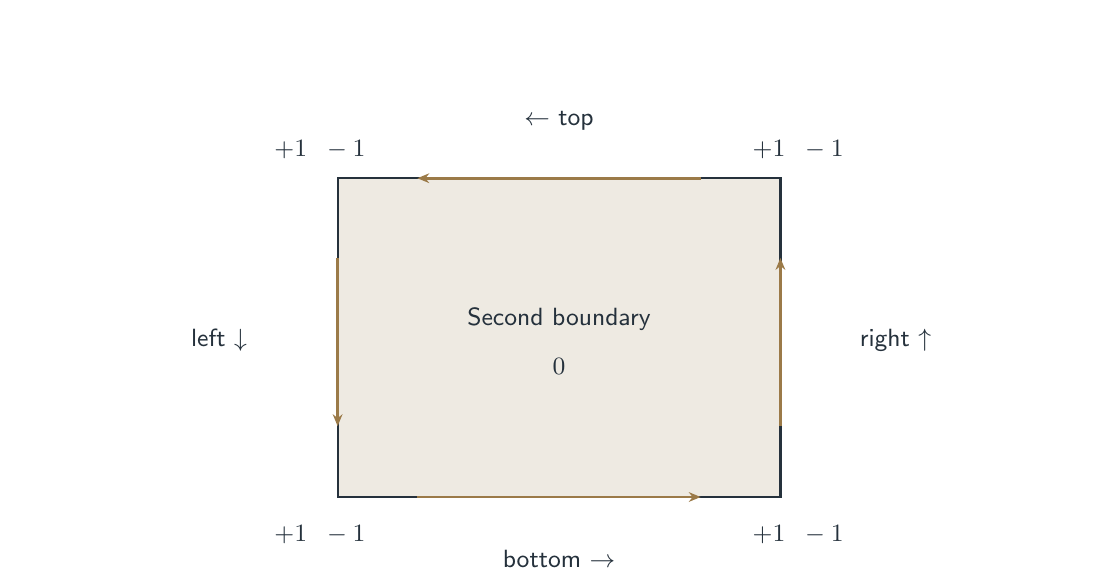
\begin{tikzpicture}[x=.64pt,y=-.64pt,derivative text]
  \path[use as bounding box] (0,0) rectangle (600,300);
  \fill[wash] (175,60) rectangle (425,240);
  \draw[derivative line] (175,240)--(425,240)--(425,60)--(175,60)--cycle;
  \draw[derivative accent,derivative arrow] (220,240)--(380,240);
  \draw[derivative accent,derivative arrow] (425,200)--(425,105);
  \draw[derivative accent,derivative arrow] (380,60)--(220,60);
  \draw[derivative accent,derivative arrow] (175,105)--(175,200);
  \node[anchor=base] at (300,280) {bottom \(\rightarrow\)};
  \node[anchor=base] at (300,30) {\(\leftarrow\) top};
  \node[anchor=base] at (108,155) {left \(\downarrow\)};
  \node[anchor=base] at (490,155) {right \(\uparrow\)};
  \foreach \px/\py in {165/48,435/48,165/265,435/265}
    \node[anchor=base] at (\px,\py) {\(+1\;\;-1\)};
  \node[anchor=base] at (300,143) {Second boundary};
  \node[anchor=base] at (300,171) {\(0\)};
\end{tikzpicture}
\caption{Corner points cancel with opposite signs. This mechanism differs from discarding the rectangle's second-order corner area; the connection is developed through graded product rules and Stokes' theorem.}
\label{fig:boundary}
\end{figure}%
}

\expandafter\def\csname derivativefigure@diagonal\endcsname{%
\begin{figure}[H]
\centering
\begin{tikzpicture}[x=.64pt,y=-.64pt,derivative text]
  \path[use as bounding box] (0,0) rectangle (600,290);
  \draw[derivative line] (120,245)--(490,245);
  \draw[derivative line] (120,245)--(120,25);
  \node[anchor=base west] at (500,250) {\(t_{\mathrm{left}}\)};
  \node[anchor=base] at (108,18) {\(t_{\mathrm{right}}\)};
  \fill[selection] (118,221)--(433,21)--(457,59)--(142,259)--cycle;
  \draw[derivative accent] (130,240)--(445,40);
  \fill[ink] (270,151) circle[radius=3.2pt];
  \fill[inkblue] (270,128) circle[radius=3.2pt];
  \draw[derivative muted] (270,151)--(270,128);
  \node[anchor=base west] at (300,135) {difference \(h\)};
  \node[anchor=base west] at (215,205) {diagonal: \(h=0\)};
  \node[anchor=base east] at (565,65) {retain \(h\), discard \(h^2\)};
\end{tikzpicture}
\caption{The marked positions keep the left coordinate fixed; their right-coordinate difference is \(h\). Removing \(h^2\) gives the universal first-order difference. The band is schematic: an algebraic infinitesimal neighborhood has no numerical thickness.}
\label{fig:diagonal}
\end{figure}%
}

% Each arithmetic panel reuses the corresponding published circle geometry.
\newcommand{\DerivativeArithmeticPanel}[1]{%
  \begin{tikzpicture}[x=.35pt,y=-.35pt,derivative text]
    \path[use as bounding box] (0,0) rectangle (600,180);
    \ifnum#1=3
      \fill[wash] (300,75) circle[radius=11.55pt];
      \node[anchor=base] at (300,81) {\(\mathbf F_9\)};
      \node[anchor=base] at (300,145) {One closed point; two geometric points};
    \else\ifnum#1=2
      \fill[selection] (300,75) circle[radius=11.9pt];
      \fill[white] (300,75) circle[radius=7pt];
      \node[anchor=base] at (300,81) {\(1\)};
      \node[anchor=base] at (300,145) {One doubled point, length \(2\)};
    \else
      \fill[selection] (190,75) circle[radius=8.4pt];
      \fill[selection] (410,75) circle[radius=8.4pt];
      \ifnum#1=13
        \node[anchor=base] at (190,81) {\(5\)};
        \node[anchor=base] at (410,81) {\(8\)};
      \else
        \node[anchor=base] at (190,81) {\(2\)};
        \node[anchor=base] at (410,81) {\(3\)};
      \fi
      \node[anchor=base] at (300,145) {Two reduced rational points};
    \fi\fi
  \end{tikzpicture}%
}
\expandafter\def\csname derivativefigure@arithmetic\endcsname{%
\begin{figure}[H]
\centering
\DerivativeState{The online default is \(p=5\); the four available states are shown here.}
\begin{minipage}[t]{.48\linewidth}\centering
  {\fontsize{10}{12}\selectfont \(p=5:\quad\mathbf F_5\times\mathbf F_5\)}\par\smallskip
  \DerivativeArithmeticPanel{5}\par
  {\fontsize{9.5}{11.5}\selectfont Relative differential module \(0\).}
\end{minipage}\hfill
\begin{minipage}[t]{.48\linewidth}\centering
  {\fontsize{10}{12}\selectfont \(p=3:\quad\mathbf F_9\)}\par\smallskip
  \DerivativeArithmeticPanel{3}\par
  {\fontsize{9.5}{11.5}\selectfont Closed-point degree \(2\); differential module \(0\).}
\end{minipage}
\par\medskip
\begin{minipage}[t]{.48\linewidth}\centering
  {\fontsize{10}{12}\selectfont \(p=2:\quad\mathbf F_2[u]/(u^2)\)}\par\smallskip
  \DerivativeArithmeticPanel{2}\par
  {\fontsize{9.5}{11.5}\selectfont A nonzero nilpotent direction; \(\Omega\cong C\,du\).}
\end{minipage}\hfill
\begin{minipage}[t]{.48\linewidth}\centering
  {\fontsize{10}{12}\selectfont \(p=13:\quad\mathbf F_{13}\times\mathbf F_{13}\)}\par\smallskip
  \DerivativeArithmeticPanel{13}\par
  {\fontsize{9.5}{11.5}\selectfont Roots \(5,8\); relative differential module \(0\).}
\end{minipage}
\caption{The doubled point at \(2\) is detected by the differential module. The degree-two point at \(3\) becomes two points after extending the residue field.}
\label{fig:arithmetic}
\end{figure}%
}

\expandafter\def\csname derivativefigure@frobenius\endcsname{%
\begin{figure}[H]
\centering
\DerivativeState{Characteristic \(3\); input \(\varepsilon\). Online default: probe order \(m=1\).}
\DerivativePowerRow{1}
\DerivativeState{Ordinary derivative \(0\qquad\) Default output \(0\qquad\) First visible Hasse order \(3\).}
{\fontsize{10}{12}\selectfont
\begin{tabularx}{.94\linewidth}{@{}cXc@{}}
\toprule
Probe order \(m\)&Retained powers&Frobenius output\\
\midrule
\(1\)&\(1,\varepsilon\)&\(0\)\\
\(2\)&\(1,\varepsilon,\varepsilon^2\)&\(0\)\\
\(3\)&\(1,\varepsilon,\varepsilon^2,\varepsilon^3\)&\(\varepsilon^3\)\\
\bottomrule
\end{tabularx}}
\caption{For \(t\mapsto t^3\) in characteristic \(3\), an increment first survives in a probe retaining cubic terms. Increasing jet order preserves more Taylor coefficients without changing the zero first derivative.}
\label{fig:frobenius}
\end{figure}%
}

\expandafter\def\csname derivativefigure@node\endcsname{%
\begin{figure}[H]
\centering
\DerivativeState{Static default: \(a=b=1\). Residual \(ab=1.0000\): second-order lift obstructed.}
\begin{tikzpicture}[x=.64pt,y=-.64pt,derivative text]
  \path[use as bounding box] (0,0) rectangle (600,290);
  \draw[derivative muted] (115,145)--(485,145);
  \draw[derivative muted] (300,20)--(300,270);
  \draw[derivative accent] (125,145)--(475,145);
  \draw[derivative accent] (300,30)--(300,260);
  \draw[inkblue,line width=1pt,derivative arrow] (300,145)--(400,45);
  \fill[ink] (300,145) circle[radius=2.56pt];
  \fill[inkblue] (400,45) circle[radius=3.2pt];
  \node[anchor=base west] at (490,150) {\(x\)};
  \node[anchor=base] at (300,15) {\(y\)};
  \node[anchor=base west] at (320,172) {\(xy=0\)};
\end{tikzpicture}
\caption{The arrow is a tangent direction, not a point of the curve. Continuing it in the fixed node requires the product of its components to vanish.}
\label{fig:node}
\end{figure}%
}

\expandafter\def\csname derivativefigure@self-intersection\endcsname{%
\begin{figure}[H]
\centering
\begin{minipage}[t]{.48\linewidth}\centering
{\fontsize{10}{12}\selectfont\sffamily Line in \(\mathbf P^2\)}\par\smallskip
\begin{tikzpicture}[x=.66pt,y=-.66pt,derivative text]
  \path[use as bounding box] (0,0) rectangle (300,260);
  \draw[derivative line] (45,145)--(255,50);
  \draw[inkblue,line width=.85pt] (45,65)--(255,140);
  \fill[accent] (143.8235,100.2941) circle[radius=3.3pt];
  \node[anchor=base] at (150,195) {Normal bundle \(\mathcal O(1)\)};
  \node[anchor=base] at (150,228) {Self-intersection \(1\)};
\end{tikzpicture}
\end{minipage}\hfill
\begin{minipage}[t]{.48\linewidth}\centering
{\fontsize{10}{12}\selectfont\sffamily Fiber in \(\mathbf P^1\times\mathbf P^1\)}\par\smallskip
\begin{tikzpicture}[x=.66pt,y=-.66pt,derivative text]
  \path[use as bounding box] (0,0) rectangle (300,260);
  \draw[derivative line] (40,95)--(265,95);
  \draw[inkblue,line width=.85pt] (40,50)--(265,50);
  \node[anchor=base] at (150,195) {Normal bundle \(\mathcal O\)};
  \node[anchor=base] at (150,228) {Self-intersection \(0\)};
\end{tikzpicture}
\end{minipage}
\caption{A schematic displacement makes the counts visible. The intrinsic curve is \(\mathbf P^1\) in both panels; the global conormal bundle distinguishes their derived self-intersections.}
\label{fig:self-intersection}
\end{figure}%
}

\expandafter\def\csname derivativefigure@probes\endcsname{%
\begin{figure}[H]
\centering
\DerivativeState{Characteristic zero; input \(x=\varepsilon\). Online default: probe order \(m=1\).}
\DerivativePowerRow{1}
\DerivativeState{Square and cube constraints: tangent dimension \(1\), obstruction target dimension \(1\).}
{\fontsize{10}{12}\selectfont
\begin{tabularx}{.94\linewidth}{@{}cXX@{}}
\toprule
Probe order&Square constraint \(x^2=0\)&Cube constraint \(x^3=0\)\\
\midrule
\(1\)&Relation satisfied; residual \(0\)&Relation satisfied; residual \(0\)\\
\(2\)&Relation fails; residual \(\varepsilon^2\)&Relation satisfied; residual \(0\)\\
\(3\)&Relation fails; residual \(\varepsilon^2\)&Relation fails; residual \(\varepsilon^3\)\\
\bottomrule
\end{tabularx}}
\caption{The two pointwise tangent complexes agree. The square relation first fails at order \(2\), the cube relation at order \(3\). Higher brackets retain the different formal compatibility laws.}
\label{fig:probes}
\end{figure}%
}

\expandafter\def\csname derivativefigure@goodwillie\endcsname{%
\begin{figure}[H]
\centering
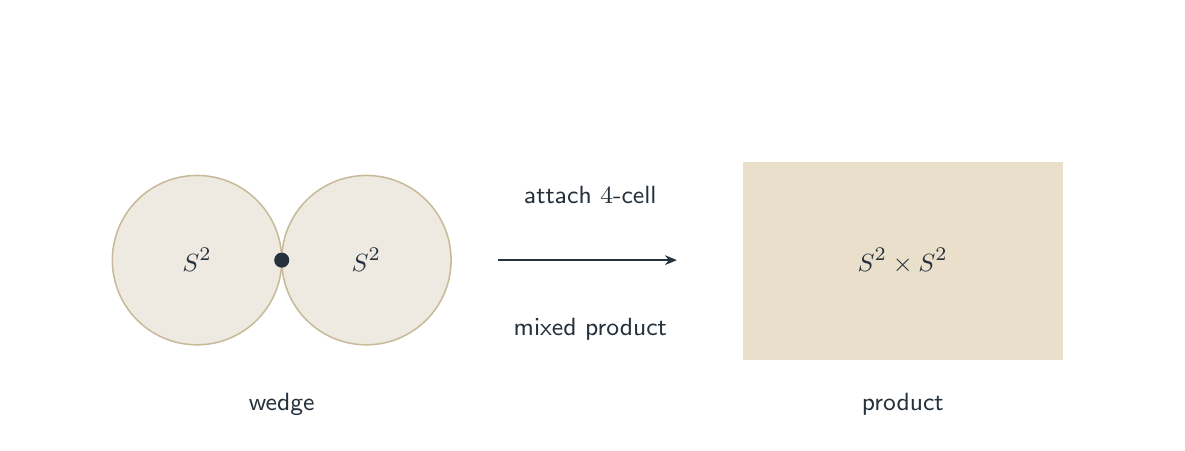
\begin{tikzpicture}[x=.68pt,y=-.68pt,derivative text]
  \path[use as bounding box] (0,0) rectangle (600,210);
  \filldraw[fill=wash,draw=frame,line width=.55pt] (90,100) circle[radius=30.6pt];
  \filldraw[fill=wash,draw=frame,line width=.55pt] (180,100) circle[radius=30.6pt];
  \fill[ink] (135,100) circle[radius=2.72pt];
  \node[anchor=base] at (90,106) {\(S^2\)};
  \node[anchor=base] at (180,106) {\(S^2\)};
  \node[anchor=base] at (135,180) {wedge};
  \draw[derivative line,derivative arrow] (250,100)--(345,100);
  \node[anchor=base] at (299,70) {attach \(4\)-cell};
  \node[anchor=base] at (299,140) {mixed product};
  \fill[selection] (380,48) rectangle (550,153);
  \node[anchor=base] at (465,106) {\(S^2\times S^2\)};
  \node[anchor=base] at (465,180) {product};
\end{tikzpicture}
\caption{The sphere outlines and product block are schematic. The relevant datum is the attaching map of the 4-cell, the mixed Whitehead product. The first stable approximation loses this interaction; the second derivative detects it.}
\label{fig:goodwillie}
\end{figure}%
}

\begin{document}
\color{ink}
\thispagestyle{empty}
{\sffamily\small\textcolor{accent}{TENSORGAMI · EXPOSITIONS}\par}
\vspace{.6em}
{\LARGE\bfseries What a Derivative Retains\par}
\vspace{.4em}
{\large\itshape From side strips and oriented boundaries\\to infinitesimal geometry\par}
\vspace{.65em}
{Henry Shin\hspace{.6em}·\hspace{.6em}October 2026\par}
\vspace{.3em}
{\small\href{https://tensorgami.com/notes/what-a-derivative-retains.html}{Tensorgami · web edition}\par}
\vspace{.8em}
{\small This PDF preserves the published exposition. Interactive exhibits appear as labeled static states and comparisons; their controls remain available in the linked web edition.\par}
\vspace{.6em}

An expanding rectangle and an oriented square give two pictures of a product rule. One separates a linear change from a quadratic corner; the other separates boundary faces and cancels their endpoints. Following these pictures leads to derivatives over arithmetic rings, defining constraints in cotangent complexes, and nonlinear interactions in homotopy theory.


The organizing question is what a first-order description retains. A scalar slope, a cotangent module, a derived fiber, and a formal deformation law retain different information. Each enlargement below is introduced by a calculation in which that difference matters. Two operations guide the route: discard products of changes to extract a linear response; retain degrees and signs to organize how pieces fit together.


The opening pictures return at the advanced steps. Fixing the rectangle's area turns the strips into a linear constraint and the corner into a possible obstruction. Higher brackets encode the rule producing that obstruction. Spectral differentiation keeps the homotopies in multiplication and in its infinitesimal responses. Goodwillie calculus applies linear approximation to gluing spaces, where a product-cell boundary exhibits the interaction that stabilization loses. These constructions enrich different parts of the original picture; their coefficient choices and reconstruction hypotheses will be stated at each step.


The opening uses calculus and elementary chains. Polynomial algebras and modules enter next; complexes and derived tensor products are introduced when ordinary quotients lose constraints. The final four sections assume familiarity with graded algebra and homotopy theory; the spectral section uses stable homotopy theory. Cohomological complexes use the convention that \(
% DERIVATIVE-MATH-BEGIN 0 inline
V[1]
% DERIVATIVE-MATH-END 0
\), for a vector space \(
% DERIVATIVE-MATH-BEGIN 1 inline
V
% DERIVATIVE-MATH-END 1
\) in degree zero, lies in degree \(
% DERIVATIVE-MATH-BEGIN 2 inline
-1
% DERIVATIVE-MATH-END 2
\).




\clearpage\thispagestyle{plain}\tableofcontents\clearpage
\section{The side strips of a rectangle}\label{sec:rectangle}\hypertarget{rectangle}{}

A rectangle has side lengths \(
% DERIVATIVE-MATH-BEGIN 3 inline
a
% DERIVATIVE-MATH-END 3
\) and \(
% DERIVATIVE-MATH-BEGIN 4 inline
b
% DERIVATIVE-MATH-END 4
\), so its area is \(
% DERIVATIVE-MATH-BEGIN 5 inline
A=ab
% DERIVATIVE-MATH-END 5
\). Change the lengths to \(
% DERIVATIVE-MATH-BEGIN 6 inline
a+\alpha h
% DERIVATIVE-MATH-END 6
\) and \(
% DERIVATIVE-MATH-BEGIN 7 inline
b+\beta h
% DERIVATIVE-MATH-END 7
\). The new area is exactly


\DerivativeDisplay{8}{
% DERIVATIVE-MATH-BEGIN 8 display
(a+\alpha h)(b+\beta h)
=ab+b\alpha h+a\beta h+\alpha\beta h^2.
% DERIVATIVE-MATH-END 8
}

For positive increments, the three added pieces are two side strips and a corner: a strip of area \(
% DERIVATIVE-MATH-BEGIN 9 inline
b\alpha h
% DERIVATIVE-MATH-END 9
\), another of area \(
% DERIVATIVE-MATH-BEGIN 10 inline
a\beta h
% DERIVATIVE-MATH-END 10
\), and a corner of area \(
% DERIVATIVE-MATH-BEGIN 11 inline
\alpha\beta h^2
% DERIVATIVE-MATH-END 11
\). The identity also holds for signed increments, with the appropriate removals of area. Dividing the change by \(
% DERIVATIVE-MATH-BEGIN 12 inline
h\ne0
% DERIVATIVE-MATH-END 12
\) gives



\DerivativeDisplay{13}{
% DERIVATIVE-MATH-BEGIN 13 display
\frac{A(h)-A(0)}h=b\alpha+a\beta+\alpha\beta h.
% DERIVATIVE-MATH-END 13
}

The limit retains the strips and discards the corner. This is already a precise answer to what a derivative keeps: the part of the change that scales linearly with the parameter.



\DerivativeFigure{rectangle}

The same calculation gives the product rule without assuming that the sides move at constant speeds. If \(
% DERIVATIVE-MATH-BEGIN 14 inline
u
% DERIVATIVE-MATH-END 14
\) and \(
% DERIVATIVE-MATH-BEGIN 15 inline
v
% DERIVATIVE-MATH-END 15
\) are differentiable at \(
% DERIVATIVE-MATH-BEGIN 16 inline
x
% DERIVATIVE-MATH-END 16
\), put \(
% DERIVATIVE-MATH-BEGIN 17 inline
\Delta u=u(x+h)-u(x)
% DERIVATIVE-MATH-END 17
\) and \(
% DERIVATIVE-MATH-BEGIN 18 inline
\Delta v=v(x+h)-v(x)
% DERIVATIVE-MATH-END 18
\). Then



\DerivativeDisplay{19}{
% DERIVATIVE-MATH-BEGIN 19 display
\Delta(uv)=v(x)\Delta u+u(x)\Delta v+\Delta u\,\Delta v.
% DERIVATIVE-MATH-END 19
}

Differentiability gives \(
% DERIVATIVE-MATH-BEGIN 20 inline
\Delta u=u'(x)h+o(|h|)
% DERIVATIVE-MATH-END 20
\) and \(
% DERIVATIVE-MATH-BEGIN 21 inline
\Delta v=v'(x)h+o(|h|)
% DERIVATIVE-MATH-END 21
\). Their product is \(
% DERIVATIVE-MATH-BEGIN 22 inline
O(h^2)
% DERIVATIVE-MATH-END 22
\), so its contribution after division by \(
% DERIVATIVE-MATH-BEGIN 23 inline
h
% DERIVATIVE-MATH-END 23
\) tends to zero. Therefore



\DerivativeDisplay{24}{
% DERIVATIVE-MATH-BEGIN 24 display
(uv)'(x)=u'(x)v(x)+u(x)v'(x).
% DERIVATIVE-MATH-END 24
}

The rectangle supplies more than a mnemonic. Its exact decomposition identifies the term that must disappear when we retain only first-order variation. Later, an algebraic infinitesimal will make that disappearance an exact quotient operation.


For example, start with side lengths \(
% DERIVATIVE-MATH-BEGIN 25 inline
3
% DERIVATIVE-MATH-END 25
\) and \(
% DERIVATIVE-MATH-BEGIN 26 inline
2
% DERIVATIVE-MATH-END 26
\), and let both increase by \(
% DERIVATIVE-MATH-BEGIN 27 inline
h
% DERIVATIVE-MATH-END 27
\). The area changes from \(
% DERIVATIVE-MATH-BEGIN 28 inline
6
% DERIVATIVE-MATH-END 28
\) to \(
% DERIVATIVE-MATH-BEGIN 29 inline
6+5h+h^2
% DERIVATIVE-MATH-END 29
\). At \(
% DERIVATIVE-MATH-BEGIN 30 inline
h=1/10
% DERIVATIVE-MATH-END 30
\), the added area is \(
% DERIVATIVE-MATH-BEGIN 31 inline
0.51
% DERIVATIVE-MATH-END 31
\): the strips contribute \(
% DERIVATIVE-MATH-BEGIN 32 inline
0.5
% DERIVATIVE-MATH-END 32
\) and the corner \(
% DERIVATIVE-MATH-BEGIN 33 inline
0.01
% DERIVATIVE-MATH-END 33
\). The derivative with respect to this common parameter is \(
% DERIVATIVE-MATH-BEGIN 34 inline
5
% DERIVATIVE-MATH-END 34
\). It depends on the chosen motion of the two sides. Allowing separate increments instead gives the differential \(
% DERIVATIVE-MATH-BEGIN 35 inline
dA=b\,da+a\,db
% DERIVATIVE-MATH-END 35
\), which can be evaluated on any such motion.



\section{The oriented boundary of the square}\label{sec:boundary}\hypertarget{boundary}{}

Now keep a rectangle fixed and ask how its boundary pieces fit together. Write it as \(
% DERIVATIVE-MATH-BEGIN 36 inline
I\times J
% DERIVATIVE-MATH-END 36
\), with \(
% DERIVATIVE-MATH-BEGIN 37 inline
I=[a,b]
% DERIVATIVE-MATH-END 37
\), \(
% DERIVATIVE-MATH-BEGIN 38 inline
J=[c,d]
% DERIVATIVE-MATH-END 38
\), \(
% DERIVATIVE-MATH-BEGIN 39 inline
a<b
% DERIVATIVE-MATH-END 39
\), and \(
% DERIVATIVE-MATH-BEGIN 40 inline
c<d
% DERIVATIVE-MATH-END 40
\); these letters now denote endpoints rather than the side lengths above. Orient both intervals in the increasing direction, and orient \(
% DERIVATIVE-MATH-BEGIN 41 inline
Q=I\times J
% DERIVATIVE-MATH-END 41
\) by the order of the coordinates. The boundary of an interval is its final endpoint minus its initial endpoint:


\DerivativeDisplay{42}{
% DERIVATIVE-MATH-BEGIN 42 display
\partial I=[b]-[a],\qquad \partial J=[d]-[c].
% DERIVATIVE-MATH-END 42
}

The square has the counterclockwise boundary



\DerivativeDisplay{43}{
% DERIVATIVE-MATH-BEGIN 43 display
\partial(I\times J)
=(\partial I)\times J-I\times(\partial J).
% DERIVATIVE-MATH-END 43
}

The first term gives the right edge upward and the left edge downward. The second gives the top edge leftward and the bottom edge rightward. The minus sign is the orientation change required when the boundary operation passes the first interval. For oriented cubical chains, the general product formula is



\DerivativeDisplay{44}{
% DERIVATIVE-MATH-BEGIN 44 display
\partial(C\times E)
=(\partial C)\times E+(-1)^{\deg C}C\times(\partial E).
% DERIVATIVE-MATH-END 44
}

Here the degree of a chain is its dimension.\hypertarget{citation-hatcher-1}{}\nobreak\hspace{.08em}\hyperlink{note-hatcher}{\textsuperscript{1}}


Apply the boundary once more. Writing \(
% DERIVATIVE-MATH-BEGIN 45 inline
[r,s]
% DERIVATIVE-MATH-END 45
\) here for the vertex at coordinates \(
% DERIVATIVE-MATH-BEGIN 46 inline
(r,s)
% DERIVATIVE-MATH-END 46
\), the eight endpoint contributions are



\DerivativeDisplay{47}{
% DERIVATIVE-MATH-BEGIN 47 display
\begin{aligned}
\partial^2Q={}&[b,d]-[b,c]-[a,d]+[a,c]\\
&-[b,d]+[a,d]+[b,c]-[a,c]=0.
\end{aligned}
% DERIVATIVE-MATH-END 47
}

Every corner occurs twice, with opposite signs. The statement \(
% DERIVATIVE-MATH-BEGIN 48 inline
\partial^2=0
% DERIVATIVE-MATH-END 48
\) records this cancellation, including its orientation data. If we retained only the unsigned set of edges and then took their endpoints, we would see four corners. Chains preserve the signs that make the second boundary vanish.



\DerivativeFigure{boundary}

The product rule for slopes and the product rule for boundaries thus share a structural feature: act on one factor at a time. The boundary carries an additional degree and its associated sign. Keeping that degree will matter when products become tensor products of complexes.


The cancellation also explains why a boundary has no boundary as a chain even when individual boundary pieces have endpoints. A right edge alone has two endpoints. Within the whole oriented square, its upper endpoint cancels the initial contribution from the top edge, and its lower endpoint cancels the terminal contribution from the bottom. The identity concerns how the pieces fit together. It is precisely this information that an unsigned picture suppresses.



\section{Differential forms and integration}\label{sec:forms}\hypertarget{forms}{}

On a smooth space, differential forms connect local differentiation with oriented boundaries. For a smooth function \(
% DERIVATIVE-MATH-BEGIN 49 inline
f(x,y)
% DERIVATIVE-MATH-END 49
\), its differential is


\DerivativeDisplay{50}{
% DERIVATIVE-MATH-BEGIN 50 display
df=\frac{\partial f}{\partial x}\,dx+
\frac{\partial f}{\partial y}\,dy.
% DERIVATIVE-MATH-END 50
}

It is a one-form: at each point it takes a tangent vector and returns the corresponding directional derivative. Forms multiply by the exterior product, with \(
% DERIVATIVE-MATH-BEGIN 51 inline
dx\wedge dy=-dy\wedge dx
% DERIVATIVE-MATH-END 51
\) and \(
% DERIVATIVE-MATH-BEGIN 52 inline
dx\wedge dx=0
% DERIVATIVE-MATH-END 52
\). The exterior derivative increases degree and obeys



\DerivativeDisplay{53}{
% DERIVATIVE-MATH-BEGIN 53 display
d(\alpha\wedge\beta)
=d\alpha\wedge\beta+(-1)^r\alpha\wedge d\beta,
\qquad \deg\alpha=r.
% DERIVATIVE-MATH-END 53
}

For two functions, both of degree zero, this is the ordinary product rule. For higher-degree forms, the sign supplies the same kind of coherence that appeared in the square's boundary.


The identity \(
% DERIVATIVE-MATH-BEGIN 54 inline
d^2=0
% DERIVATIVE-MATH-END 54
\) depends on this exterior algebra. For \(
% DERIVATIVE-MATH-BEGIN 55 inline
f=x^2
% DERIVATIVE-MATH-END 55
\),



\DerivativeDisplay{56}{
% DERIVATIVE-MATH-BEGIN 56 display
df=2x\,dx,\qquad d(df)=2\,dx\wedge dx=0,
% DERIVATIVE-MATH-END 56
}

whereas the ordinary second derivative \(
% DERIVATIVE-MATH-BEGIN 57 inline
D^2f=2
% DERIVATIVE-MATH-END 57
\). The Hessian still carries second-order variation. Applying the exterior derivative twice instead antisymmetrizes second partial derivatives, and their symmetry makes the result vanish.


Stokes' theorem connects the two square-zero operations through integration:



\DerivativeDisplay{58}{
% DERIVATIVE-MATH-BEGIN 58 display
\int_Q d\omega=\int_{\partial Q}\omega.
% DERIVATIVE-MATH-END 58
}

For a compact oriented smooth manifold with boundary, this holds for smooth forms of the appropriate degree; the familiar version also allows a rectangular domain with piecewise smooth boundary.\hypertarget{citation-stokes-1}{}\nobreak\hspace{.08em}\hyperlink{note-stokes}{\textsuperscript{2}} Take \(
% DERIVATIVE-MATH-BEGIN 59 inline
\omega=x\,dy
% DERIVATIVE-MATH-END 59
\) on our rectangle. Then \(
% DERIVATIVE-MATH-BEGIN 60 inline
d\omega=dx\wedge dy
% DERIVATIVE-MATH-END 60
\), and



\DerivativeDisplay{61}{
% DERIVATIVE-MATH-BEGIN 61 display
\int_Qd\omega=(b-a)(d-c).
% DERIVATIVE-MATH-END 61
}

The horizontal edges contribute zero because \(
% DERIVATIVE-MATH-BEGIN 62 inline
dy=0
% DERIVATIVE-MATH-END 62
\). The right edge contributes \(
% DERIVATIVE-MATH-BEGIN 63 inline
b(d-c)
% DERIVATIVE-MATH-END 63
\), and the downward left edge contributes \(
% DERIVATIVE-MATH-BEGIN 64 inline
a(c-d)
% DERIVATIVE-MATH-END 64
\). Hence



\DerivativeDisplay{65}{
% DERIVATIVE-MATH-BEGIN 65 display
\int_{\partial Q}x\,dy=b(d-c)+a(c-d)=(b-a)(d-c).
% DERIVATIVE-MATH-END 65
}

The boundary and the exterior derivative are paired operations: one lowers geometric dimension, the other raises the degree of a measurement. Integration identifies their outputs. A topological space already admits chains and boundaries; defining ordinary tangent derivatives additionally requires an appropriate smooth, analytic, or algebraic structure. The next step extracts the algebraic structure responsible for the first-order product rule.



\section{The universal derivation and the diagonal}\label{sec:kahler}\hypertarget{kahler}{}

The strip calculation used addition, multiplication, and the removal of products of changes. We can retain precisely those operations over any coefficient ring. Let \(
% DERIVATIVE-MATH-BEGIN 66 inline
k
% DERIVATIVE-MATH-END 66
\) be a commutative ring, \(
% DERIVATIVE-MATH-BEGIN 67 inline
A
% DERIVATIVE-MATH-END 67
\) a commutative \(
% DERIVATIVE-MATH-BEGIN 68 inline
k
% DERIVATIVE-MATH-END 68
\)-algebra, and \(
% DERIVATIVE-MATH-BEGIN 69 inline
M
% DERIVATIVE-MATH-END 69
\) an \(
% DERIVATIVE-MATH-BEGIN 70 inline
A
% DERIVATIVE-MATH-END 70
\)-module. A \(
% DERIVATIVE-MATH-BEGIN 71 inline
k
% DERIVATIVE-MATH-END 71
\)-derivation is a \(
% DERIVATIVE-MATH-BEGIN 72 inline
k
% DERIVATIVE-MATH-END 72
\)-linear map \(
% DERIVATIVE-MATH-BEGIN 73 inline
D:A\to M
% DERIVATIVE-MATH-END 73
\) satisfying


\DerivativeDisplay{74}{
% DERIVATIVE-MATH-BEGIN 74 display
D(ab)=aD(b)+bD(a).
% DERIVATIVE-MATH-END 74
}

The module of Kähler differentials \(
% DERIVATIVE-MATH-BEGIN 75 inline
\Omega_{A/k}
% DERIVATIVE-MATH-END 75
\) is generated by symbols \(
% DERIVATIVE-MATH-BEGIN 76 inline
da
% DERIVATIVE-MATH-END 76
\), subject to additivity, this product rule, and \(
% DERIVATIVE-MATH-BEGIN 77 inline
dc=0
% DERIVATIVE-MATH-END 77
\) for scalars \(
% DERIVATIVE-MATH-BEGIN 78 inline
c\in k
% DERIVATIVE-MATH-END 78
\). The resulting map \(
% DERIVATIVE-MATH-BEGIN 79 inline
d:A\to\Omega_{A/k}
% DERIVATIVE-MATH-END 79
\) is universal:



\DerivativeDisplay{80}{
% DERIVATIVE-MATH-BEGIN 80 display
\operatorname{Hom}_A(\Omega_{A/k},M)
\cong\operatorname{Der}_k(A,M).
% DERIVATIVE-MATH-END 80
}

Every derivation factors uniquely through \(
% DERIVATIVE-MATH-BEGIN 81 inline
d
% DERIVATIVE-MATH-END 81
\). The module retains all compatible first-order measurements at once; choosing a map from it to \(
% DERIVATIVE-MATH-BEGIN 82 inline
M
% DERIVATIVE-MATH-END 82
\) chooses one way to read them.\hypertarget{citation-stacks-diff-1}{}\nobreak\hspace{.08em}\hyperlink{note-stacks-diff}{\textsuperscript{3}}


For \(
% DERIVATIVE-MATH-BEGIN 83 inline
A=k[t]
% DERIVATIVE-MATH-END 83
\), this gives \(
% DERIVATIVE-MATH-BEGIN 84 inline
\Omega_{A/k}=A\,dt
% DERIVATIVE-MATH-END 84
\). Repeated use of the product rule yields



\DerivativeDisplay{85}{
% DERIVATIVE-MATH-BEGIN 85 display
d(t^n)=nt^{n-1}\,dt,\qquad df=f'(t)\,dt
% DERIVATIVE-MATH-END 85
}

for every polynomial \(
% DERIVATIVE-MATH-BEGIN 86 inline
f
% DERIVATIVE-MATH-END 86
\). Thus the familiar coefficient \(
% DERIVATIVE-MATH-BEGIN 87 inline
f'(t)
% DERIVATIVE-MATH-END 87
\) appears after choosing the coordinate \(
% DERIVATIVE-MATH-BEGIN 88 inline
t
% DERIVATIVE-MATH-END 88
\). The universal differential \(
% DERIVATIVE-MATH-BEGIN 89 inline
df
% DERIVATIVE-MATH-END 89
\) is the object before that coordinate presentation.


There is a geometric construction of the same module. Form \(
% DERIVATIVE-MATH-BEGIN 90 inline
B=A\otimes_kA
% DERIVATIVE-MATH-END 90
\), let \(
% DERIVATIVE-MATH-BEGIN 91 inline
\mu:B\to A
% DERIVATIVE-MATH-END 91
\) multiply the factors, and put \(
% DERIVATIVE-MATH-BEGIN 92 inline
I=\ker\mu
% DERIVATIVE-MATH-END 92
\). The two copies of \(
% DERIVATIVE-MATH-BEGIN 93 inline
A
% DERIVATIVE-MATH-END 93
\) agree on the diagonal. Their differences



\DerivativeDisplay{94}{
% DERIVATIVE-MATH-BEGIN 94 display
\delta a=1\otimes a-a\otimes1
% DERIVATIVE-MATH-END 94
}

generate the ideal \(
% DERIVATIVE-MATH-BEGIN 95 inline
I
% DERIVATIVE-MATH-END 95
\). In \(
% DERIVATIVE-MATH-BEGIN 96 inline
B
% DERIVATIVE-MATH-END 96
\), an exact multiplication identity gives



\DerivativeDisplay{97}{
% DERIVATIVE-MATH-BEGIN 97 display
\delta(ab)=(a\otimes1)\delta b+(b\otimes1)\delta a+
\delta a\,\delta b.
% DERIVATIVE-MATH-END 97
}

Pass to \(
% DERIVATIVE-MATH-BEGIN 98 inline
I/I^2
% DERIVATIVE-MATH-END 98
\). The last term disappears, just as the rectangle's corner disappeared, and the remaining terms satisfy the derivation rule. This produces a map \(
% DERIVATIVE-MATH-BEGIN 99 inline
\Omega_{A/k}\to I/I^2
% DERIVATIVE-MATH-END 99
\).


To see that it is an isomorphism, use the square-zero algebra \(
% DERIVATIVE-MATH-BEGIN 100 inline
A\oplus\Omega_{A/k}
% DERIVATIVE-MATH-END 100
\), with multiplication



\DerivativeDisplay{101}{
% DERIVATIVE-MATH-BEGIN 101 display
(a,\eta)(b,\theta)=(ab,a\theta+b\eta).
% DERIVATIVE-MATH-END 101
}

The map \(
% DERIVATIVE-MATH-BEGIN 102 inline
a\otimes b\mapsto(ab,a\,db)
% DERIVATIVE-MATH-END 102
\) is an algebra homomorphism. It sends \(
% DERIVATIVE-MATH-BEGIN 103 inline
I
% DERIVATIVE-MATH-END 103
\) into \(
% DERIVATIVE-MATH-BEGIN 104 inline
0\oplus\Omega_{A/k}
% DERIVATIVE-MATH-END 104
\), kills \(
% DERIVATIVE-MATH-BEGIN 105 inline
I^2
% DERIVATIVE-MATH-END 105
\), and sends \(
% DERIVATIVE-MATH-BEGIN 106 inline
\delta a
% DERIVATIVE-MATH-END 106
\) to \(
% DERIVATIVE-MATH-BEGIN 107 inline
da
% DERIVATIVE-MATH-END 107
\). It therefore supplies an inverse on the generators:



\DerivativeDisplay{108}{
% DERIVATIVE-MATH-BEGIN 108 display
\Omega_{A/k}\cong I/I^2.
% DERIVATIVE-MATH-END 108
}

The differential measures first-order separation along the diagonal. For a polynomial algebra, the two tensor factors really are independent coordinate copies. The quotient keeps their linear differences and removes products of those differences. No norm or limiting process is needed.



\DerivativeFigure{diagonal}

For \(
% DERIVATIVE-MATH-BEGIN 109 inline
A=k[t]
% DERIVATIVE-MATH-END 109
\), write the two coordinates as \(
% DERIVATIVE-MATH-BEGIN 110 inline
t_1,t_2
% DERIVATIVE-MATH-END 110
\). Then \(
% DERIVATIVE-MATH-BEGIN 111 inline
B=k[t_1,t_2]
% DERIVATIVE-MATH-END 111
\), \(
% DERIVATIVE-MATH-BEGIN 112 inline
I=(t_2-t_1)
% DERIVATIVE-MATH-END 112
\), and the first infinitesimal neighborhood of the diagonal has coordinate ring



\DerivativeDisplay{113}{
% DERIVATIVE-MATH-BEGIN 113 display
k[t_1,t_2]/(t_2-t_1)^2.
% DERIVATIVE-MATH-END 113
}

Set \(
% DERIVATIVE-MATH-BEGIN 114 inline
\varepsilon=t_2-t_1
% DERIVATIVE-MATH-END 114
\). Every polynomial satisfies



\DerivativeDisplay{115}{
% DERIVATIVE-MATH-BEGIN 115 display
f(t_2)-f(t_1)=f'(t_1)\varepsilon
\quad\text{modulo }\varepsilon^2.
% DERIVATIVE-MATH-END 115
}

This is the rectangle's linear truncation in an algebraic form. The full difference still exists before taking the quotient. The quotient records an explicitly chosen level of resolution; it does not declare that the original polynomial had no higher terms.



\section{Infinitesimal points and the classical derivative}\label{sec:tangent}\hypertarget{tangent}{}

The diagonal quotient retained a universal first-order difference. To read a particular motion from it, fix a point and let functions respond to an infinitesimal displacement. Let \(
% DERIVATIVE-MATH-BEGIN 116 inline
k
% DERIVATIVE-MATH-END 116
\) now be a field, let \(
% DERIVATIVE-MATH-BEGIN 117 inline
A
% DERIVATIVE-MATH-END 117
\) be a finite-type \(
% DERIVATIVE-MATH-BEGIN 118 inline
k
% DERIVATIVE-MATH-END 118
\)-algebra, and let \(
% DERIVATIVE-MATH-BEGIN 119 inline
p:A\to k
% DERIVATIVE-MATH-END 119
\) be a \(
% DERIVATIVE-MATH-BEGIN 120 inline
k
% DERIVATIVE-MATH-END 120
\)-valued point. The dual numbers \(
% DERIVATIVE-MATH-BEGIN 121 inline
k[\varepsilon]/(\varepsilon^2)
% DERIVATIVE-MATH-END 121
\) contain a nonzero infinitesimal whose square vanishes. A first-order displacement of \(
% DERIVATIVE-MATH-BEGIN 122 inline
p
% DERIVATIVE-MATH-END 122
\) is a lift


\DerivativeDisplay{123}{
% DERIVATIVE-MATH-BEGIN 123 display
a\longmapsto p(a)+\varepsilon v(a).
% DERIVATIVE-MATH-END 123
}

It is a \(
% DERIVATIVE-MATH-BEGIN 124 inline
k
% DERIVATIVE-MATH-END 124
\)-algebra homomorphism precisely when \(
% DERIVATIVE-MATH-BEGIN 125 inline
v
% DERIVATIVE-MATH-END 125
\) is \(
% DERIVATIVE-MATH-BEGIN 126 inline
k
% DERIVATIVE-MATH-END 126
\)-linear and satisfies



\DerivativeDisplay{127}{
% DERIVATIVE-MATH-BEGIN 127 display
v(ab)=p(a)v(b)+p(b)v(a).
% DERIVATIVE-MATH-END 127
}

Thus a tangent vector is a derivation with the module action evaluated at the point. For \(
% DERIVATIVE-MATH-BEGIN 128 inline
A=k[t]
% DERIVATIVE-MATH-END 128
\), \(
% DERIVATIVE-MATH-BEGIN 129 inline
p(t)=x
% DERIVATIVE-MATH-END 129
\), and \(
% DERIVATIVE-MATH-BEGIN 130 inline
v(t)=u
% DERIVATIVE-MATH-END 130
\), the lift sends \(
% DERIVATIVE-MATH-BEGIN 131 inline
t
% DERIVATIVE-MATH-END 131
\) to \(
% DERIVATIVE-MATH-BEGIN 132 inline
x+\varepsilon u
% DERIVATIVE-MATH-END 132
\), and polynomial multiplication gives the exact identity



\DerivativeDisplay{133}{
% DERIVATIVE-MATH-BEGIN 133 display
f(x+\varepsilon u)=f(x)+\varepsilon f'(x)u.
% DERIVATIVE-MATH-END 133
}

The first-order coefficient is the directional derivative. The higher powers vanish in the testing algebra.


Put \(
% DERIVATIVE-MATH-BEGIN 134 inline
\mathfrak m=\ker p
% DERIVATIVE-MATH-END 134
\). A point derivation kills \(
% DERIVATIVE-MATH-BEGIN 135 inline
\mathfrak m^2
% DERIVATIVE-MATH-END 135
\), because both factors vanish at \(
% DERIVATIVE-MATH-BEGIN 136 inline
p
% DERIVATIVE-MATH-END 136
\). Conversely, every linear functional on \(
% DERIVATIVE-MATH-BEGIN 137 inline
\mathfrak m/\mathfrak m^2
% DERIVATIVE-MATH-END 137
\) defines such a derivation by applying it to \(
% DERIVATIVE-MATH-BEGIN 138 inline
[a-p(a)]
% DERIVATIVE-MATH-END 138
\). Hence



\DerivativeDisplay{139}{
% DERIVATIVE-MATH-BEGIN 139 display
T_p=\operatorname{Hom}_k(\mathfrak m/\mathfrak m^2,k),
\qquad
T_p^*=\mathfrak m/\mathfrak m^2
\cong\Omega_{A/k}\otimes_Ak.
% DERIVATIVE-MATH-END 139
}

The hypothesis that \(
% DERIVATIVE-MATH-BEGIN 140 inline
p
% DERIVATIVE-MATH-END 140
\) is \(
% DERIVATIVE-MATH-BEGIN 141 inline
k
% DERIVATIVE-MATH-END 141
\)-valued matters: at a general scheme point, differentials of the residue field over \(
% DERIVATIVE-MATH-BEGIN 142 inline
k
% DERIVATIVE-MATH-END 142
\) also enter the comparison. The pointwise differential is \(
% DERIVATIVE-MATH-BEGIN 143 inline
d_pf=[f-f(p)]
% DERIVATIVE-MATH-END 143
\), and \(
% DERIVATIVE-MATH-BEGIN 144 inline
v(f)
% DERIVATIVE-MATH-END 144
\) is its evaluation on \(
% DERIVATIVE-MATH-BEGIN 145 inline
v
% DERIVATIVE-MATH-END 145
\).


A morphism \(
% DERIVATIVE-MATH-BEGIN 146 inline
F:X\to Y
% DERIVATIVE-MATH-END 146
\) of \(
% DERIVATIVE-MATH-BEGIN 147 inline
k
% DERIVATIVE-MATH-END 147
\)-schemes pulls functions backward. Its differential accordingly begins as a map on cotangents,



\DerivativeDisplay{148}{
% DERIVATIVE-MATH-BEGIN 148 display
F^*\Omega_{Y/k}\longrightarrow\Omega_{X/k},
\qquad da\longmapsto d(F^*a).
% DERIVATIVE-MATH-END 148
}

Dualizing at a \(
% DERIVATIVE-MATH-BEGIN 149 inline
k
% DERIVATIVE-MATH-END 149
\)-valued point produces \(
% DERIVATIVE-MATH-BEGIN 150 inline
dF_p:T_pX\to T_{F(p)}Y
% DERIVATIVE-MATH-END 150
\). Pullbacks compose, giving the chain rule. For \(
% DERIVATIVE-MATH-BEGIN 151 inline
s=f(t)
% DERIVATIVE-MATH-END 151
\), it sends \(
% DERIVATIVE-MATH-BEGIN 152 inline
ds
% DERIVATIVE-MATH-END 152
\) to \(
% DERIVATIVE-MATH-BEGIN 153 inline
f'(t)dt
% DERIVATIVE-MATH-END 153
\); composing with \(
% DERIVATIVE-MATH-BEGIN 154 inline
z=g(s)
% DERIVATIVE-MATH-END 154
\) gives



\DerivativeDisplay{155}{
% DERIVATIVE-MATH-BEGIN 155 display
d(g(f(t)))=g'(f(t))f'(t)\,dt.
% DERIVATIVE-MATH-END 155
}

We can now return to the analytic definition. For a smooth real function near \(
% DERIVATIVE-MATH-BEGIN 156 inline
x
% DERIVATIVE-MATH-END 156
\), Taylor's formula gives



\DerivativeDisplay{157}{
% DERIVATIVE-MATH-BEGIN 157 display
f(x+h)=f(x)+f'(x)h+h^2r(h),
% DERIVATIVE-MATH-END 157
}

with \(
% DERIVATIVE-MATH-BEGIN 158 inline
r
% DERIVATIVE-MATH-END 158
\) smooth near zero. In the local ring of smooth germs, \(
% DERIVATIVE-MATH-BEGIN 159 inline
h^2r(h)\in\mathfrak m^2
% DERIVATIVE-MATH-END 159
\), so \(
% DERIVATIVE-MATH-BEGIN 160 inline
d_xf=f'(x)[h]
% DERIVATIVE-MATH-END 160
\). Analytically, the same remainder satisfies \(
% DERIVATIVE-MATH-BEGIN 161 inline
h^2r(h)=o(|h|)
% DERIVATIVE-MATH-END 161
\). The infinitesimal class and the limit recover the same first-order coefficient. For a merely differentiable function, the weaker remainder condition \(
% DERIVATIVE-MATH-BEGIN 162 inline
o(|h|)
% DERIVATIVE-MATH-END 162
\) still defines its derivative; it need not give membership in the square of an ideal of smooth or \(
% DERIVATIVE-MATH-BEGIN 163 inline
C^1
% DERIVATIVE-MATH-END 163
\) germs.


For example, the \(
% DERIVATIVE-MATH-BEGIN 164 inline
C^1
% DERIVATIVE-MATH-END 164
\) germ \(
% DERIVATIVE-MATH-BEGIN 165 inline
f(h)=|h|^{3/2}
% DERIVATIVE-MATH-END 165
\) has derivative zero at the origin and satisfies \(
% DERIVATIVE-MATH-BEGIN 166 inline
f(h)=o(|h|)
% DERIVATIVE-MATH-END 166
\). Every finite sum of products of two vanishing \(
% DERIVATIVE-MATH-BEGIN 167 inline
C^1
% DERIVATIVE-MATH-END 167
\) germs is \(
% DERIVATIVE-MATH-BEGIN 168 inline
O(h^2)
% DERIVATIVE-MATH-END 168
\), whereas this germ is not. Thus the analytic first-order remainder can vanish faster than \(
% DERIVATIVE-MATH-BEGIN 169 inline
|h|
% DERIVATIVE-MATH-END 169
\) without belonging to \(
% DERIVATIVE-MATH-BEGIN 170 inline
\mathfrak m^2
% DERIVATIVE-MATH-END 170
\).


In the ring of \(
% DERIVATIVE-MATH-BEGIN 171 inline
C^1
% DERIVATIVE-MATH-END 171
\) germs at zero, the classes \(
% DERIVATIVE-MATH-BEGIN 172 inline
[h]
% DERIVATIVE-MATH-END 172
\) and \(
% DERIVATIVE-MATH-BEGIN 173 inline
[|h|^{3/2}]
% DERIVATIVE-MATH-END 173
\) are linearly independent in \(
% DERIVATIVE-MATH-BEGIN 174 inline
\mathfrak m/\mathfrak m^2
% DERIVATIVE-MATH-END 174
\). Differentiating a relation \(
% DERIVATIVE-MATH-BEGIN 175 inline
a h+b|h|^{3/2}\in\mathfrak m^2
% DERIVATIVE-MATH-END 175
\) at zero forces \(
% DERIVATIVE-MATH-BEGIN 176 inline
a=0
% DERIVATIVE-MATH-END 176
\), since every product of two vanishing germs has derivative zero; the preceding \(
% DERIVATIVE-MATH-BEGIN 177 inline
O(h^2)
% DERIVATIVE-MATH-END 177
\) argument then forces \(
% DERIVATIVE-MATH-BEGIN 178 inline
b=0
% DERIVATIVE-MATH-END 178
\). This algebraic cotangent space is therefore larger than the one-dimensional classical cotangent space. An algebraic point derivation can distinguish the class \(
% DERIVATIVE-MATH-BEGIN 179 inline
[|h|^{3/2}]
% DERIVATIVE-MATH-END 179
\) even though its classical derivative is zero. The function algebra and the chain rules required of its derivations determine which first-order measurements are permitted.


In the smooth case, the remainder above can be written explicitly as



\DerivativeDisplay{180}{
% DERIVATIVE-MATH-BEGIN 180 display
r(h)=\int_0^1(1-s)f''(x+sh)\,ds.
% DERIVATIVE-MATH-END 180
}

For several variables, the corresponding expansion shows that the coordinate differences \(
% DERIVATIVE-MATH-BEGIN 181 inline
h_1,\ldots,h_n
% DERIVATIVE-MATH-END 181
\) form a basis of \(
% DERIVATIVE-MATH-BEGIN 182 inline
\mathfrak m/\mathfrak m^2
% DERIVATIVE-MATH-END 182
\), and



\DerivativeDisplay{183}{
% DERIVATIVE-MATH-BEGIN 183 display
d_pf=\sum_i\partial_i f(p)[h_i].
% DERIVATIVE-MATH-END 183
}

Pairing this class with a vector \(
% DERIVATIVE-MATH-BEGIN 184 inline
(v_1,\ldots,v_n)
% DERIVATIVE-MATH-END 184
\) gives \(
% DERIVATIVE-MATH-BEGIN 185 inline
\sum_i\partial_i f(p)v_i
% DERIVATIVE-MATH-END 185
\). The result is the usual linear approximation in every direction, assembled into one covector. The little-\(
% DERIVATIVE-MATH-BEGIN 186 inline
o
% DERIVATIVE-MATH-END 186
\) condition makes that approximation unique: two candidate linear maps would have a difference that is both linear in \(
% DERIVATIVE-MATH-BEGIN 187 inline
h
% DERIVATIVE-MATH-END 187
\) and \(
% DERIVATIVE-MATH-BEGIN 188 inline
o(\lVert h\rVert)
% DERIVATIVE-MATH-END 188
\), so evaluation along each fixed direction forces their difference to vanish.


For global smooth geometry, the suitable universal differential also respects every smooth chain rule. This uses the \(
% DERIVATIVE-MATH-BEGIN 189 inline
C^\infty
% DERIVATIVE-MATH-END 189
\)-ring structure on smooth functions, and its cotangent module gives ordinary smooth one-forms. The ordinary algebraic Kähler module of the underlying real algebra need not coincide with that module.\hypertarget{citation-joyce-1}{}\nobreak\hspace{.08em}\hyperlink{note-joyce}{\textsuperscript{4}} The pointwise smooth-germ construction above gives the usual cotangent vectors directly. We have reached classical differentiation through a universal construction, while keeping track of the structure that makes the return valid.



\section{An arithmetic derivative in the Gaussian integers}\label{sec:arithmetic-derivative}\hypertarget{arithmetic-derivative}{}

The square-zero test for a derivative requires no distance or limit. We can therefore replace real coordinates with arithmetic coefficients and ask which infinitesimal motions respect an equation. Consider


\DerivativeDisplay{190}{
% DERIVATIVE-MATH-BEGIN 190 display
B=\mathbf Z[i]=\mathbf Z[t]/(t^2+1).
% DERIVATIVE-MATH-END 190
}

We differentiate relative to \(
% DERIVATIVE-MATH-BEGIN 191 inline
\mathbf Z
% DERIVATIVE-MATH-END 191
\), so integers have differential zero. The defining relation gives


\DerivativeDisplay{192}{
% DERIVATIVE-MATH-BEGIN 192 display
0=d(i^2+1)=2i\,di.
% DERIVATIVE-MATH-END 192
}

Since \(
% DERIVATIVE-MATH-BEGIN 193 inline
i
% DERIVATIVE-MATH-END 193
\) is a unit, the universal module is


\DerivativeDisplay{194}{
% DERIVATIVE-MATH-BEGIN 194 display
\boxed{\Omega_{B/\mathbf Z}\cong (B/2B)\,di.}
% DERIVATIVE-MATH-END 194
}

This derivative takes values in a torsion module. Wherever \(
% DERIVATIVE-MATH-BEGIN 195 inline
2
% DERIVATIVE-MATH-END 195
\) is invertible, the module vanishes: the equation determines \(
% DERIVATIVE-MATH-BEGIN 196 inline
i
% DERIVATIVE-MATH-END 196
\) with no relative first-order freedom. At the prime above \(
% DERIVATIVE-MATH-BEGIN 197 inline
2
% DERIVATIVE-MATH-END 197
\), that infinitesimal rigidity fails.\hypertarget{citation-stacks-diff-2}{}\nobreak\hspace{.08em}\hyperlink{note-stacks-diff}{\textsuperscript{3}}
The universal property says exactly what this means for a measurement. A derivation into a \(
% DERIVATIVE-MATH-BEGIN 198 inline
B
% DERIVATIVE-MATH-END 198
\)-module \(
% DERIVATIVE-MATH-BEGIN 199 inline
M
% DERIVATIVE-MATH-END 199
\) is determined by \(
% DERIVATIVE-MATH-BEGIN 200 inline
D(i)=m
% DERIVATIVE-MATH-END 200
\), and the equation requires \(
% DERIVATIVE-MATH-BEGIN 201 inline
2i\,m=0
% DERIVATIVE-MATH-END 201
\), equivalently \(
% DERIVATIVE-MATH-BEGIN 202 inline
2m=0
% DERIVATIVE-MATH-END 202
\). For \(
% DERIVATIVE-MATH-BEGIN 203 inline
a,b\in\mathbf Z
% DERIVATIVE-MATH-END 203
\), it then gives \(
% DERIVATIVE-MATH-BEGIN 204 inline
D(a+bi)=bm
% DERIVATIVE-MATH-END 204
\). Into the torsion-free module \(
% DERIVATIVE-MATH-BEGIN 205 inline
B
% DERIVATIVE-MATH-END 205
\), every such derivation vanishes. Into \(
% DERIVATIVE-MATH-BEGIN 206 inline
B/2B
% DERIVATIVE-MATH-END 206
\), there are nonzero ones. The infinitesimal response depends on the module used to receive it. Retaining the universal module makes all those possible responses available, instead of declaring that the derivative is zero after choosing only a torsion-free target.


The module also identifies an arithmetic invariant. Its annihilator is the ideal \(
% DERIVATIVE-MATH-BEGIN 207 inline
(2i)=(2)
% DERIVATIVE-MATH-END 207
\), which is the different of \(
% DERIVATIVE-MATH-BEGIN 208 inline
\mathbf Z[i]
% DERIVATIVE-MATH-END 208
\) over \(
% DERIVATIVE-MATH-BEGIN 209 inline
\mathbf Z
% DERIVATIVE-MATH-END 209
\). Its norm is \(
% DERIVATIVE-MATH-BEGIN 210 inline
4
% DERIVATIVE-MATH-END 210
\), the absolute value of the discriminant \(
% DERIVATIVE-MATH-BEGIN 211 inline
-4
% DERIVATIVE-MATH-END 211
\). The different marks the ramified locus; here



\DerivativeDisplay{212}{
% DERIVATIVE-MATH-BEGIN 212 display
2=-i(1+i)^2,
% DERIVATIVE-MATH-END 212
}

so there is one prime ideal \(
% DERIVATIVE-MATH-BEGIN 213 inline
(1+i)
% DERIVATIVE-MATH-END 213
\) above \(
% DERIVATIVE-MATH-BEGIN 214 inline
2
% DERIVATIVE-MATH-END 214
\), appearing with multiplicity two.\hypertarget{citation-different-1}{}\nobreak\hspace{.08em}\hyperlink{note-different}{\textsuperscript{5}} Polynomial differentiation has become a way to locate arithmetic ramification.

Reducing the equation modulo primes makes this visible. Modulo \(
% DERIVATIVE-MATH-BEGIN 215 inline
5
% DERIVATIVE-MATH-END 215
\),



\DerivativeDisplay{216}{
% DERIVATIVE-MATH-BEGIN 216 display
t^2+1=(t-2)(t+2),\qquad
B\otimes_{\mathbf Z}\mathbf F_5\cong\mathbf F_5\times\mathbf F_5.
% DERIVATIVE-MATH-END 216
}

The fiber consists of two reduced rational points. Modulo \(
% DERIVATIVE-MATH-BEGIN 217 inline
3
% DERIVATIVE-MATH-END 217
\), the polynomial is irreducible, so the fiber is \(
% DERIVATIVE-MATH-BEGIN 218 inline
\operatorname{Spec}\mathbf F_9
% DERIVATIVE-MATH-END 218
\): one closed point of degree two. After extending scalars to an algebraic closure, it becomes two distinct geometric points. Both odd-prime fibers have vanishing differentials relative to their base fields, because each field factor is separable over its base field.

Modulo \(
% DERIVATIVE-MATH-BEGIN 219 inline
2
% DERIVATIVE-MATH-END 219
\), put \(
% DERIVATIVE-MATH-BEGIN 220 inline
u=t+1
% DERIVATIVE-MATH-END 220
\). Then



\DerivativeDisplay{221}{
% DERIVATIVE-MATH-BEGIN 221 display
t^2+1=(t+1)^2,\qquad
B\otimes_{\mathbf Z}\mathbf F_2\cong C:=\mathbf F_2[u]/(u^2).
% DERIVATIVE-MATH-END 221
}

There is one doubled point. Differentiating \(
% DERIVATIVE-MATH-BEGIN 222 inline
u^2=0
% DERIVATIVE-MATH-END 222
\) gives no relation in characteristic two, and


\DerivativeDisplay{223}{
% DERIVATIVE-MATH-BEGIN 223 display
\Omega_{C/\mathbf F_2}=C\,du.
% DERIVATIVE-MATH-END 223
}

The geometric sheets have merged, and the infinitesimal structure retains the failure of separation.


\DerivativeFigure{arithmetic}

There is a derived refinement of the same calculation. The cotangent complex, defined below, is



\DerivativeDisplay{224}{
% DERIVATIVE-MATH-BEGIN 224 display
\mathbb L_{B/\mathbf Z}\simeq
\left[B\xrightarrow{\,2i\,}B\right]
% DERIVATIVE-MATH-END 224
}

in degrees \(
% DERIVATIVE-MATH-BEGIN 225 inline
-1,0
% DERIVATIVE-MATH-END 225
\). For a two-term complex \(
% DERIVATIVE-MATH-BEGIN 226 inline
[E^{-1}\xrightarrow{q}E^0]
% DERIVATIVE-MATH-END 226
\), cohomology means \(
% DERIVATIVE-MATH-BEGIN 227 inline
H^{-1}=\ker q
% DERIVATIVE-MATH-END 227
\) and \(
% DERIVATIVE-MATH-BEGIN 228 inline
H^0=\operatorname{coker}q
% DERIVATIVE-MATH-END 228
\). Globally the map \(
% DERIVATIVE-MATH-BEGIN 229 inline
2i
% DERIVATIVE-MATH-END 229
\) is injective, so this complex has only \(
% DERIVATIVE-MATH-BEGIN 230 inline
\Omega_{B/\mathbf Z}
% DERIVATIVE-MATH-END 230
\) as its cohomology. Because both terms of the displayed complex are free \(
% DERIVATIVE-MATH-BEGIN 231 inline
B
% DERIVATIVE-MATH-END 231
\)-modules, its derived fiber is computed by tensoring the whole complex with \(
% DERIVATIVE-MATH-BEGIN 232 inline
\mathbf F_2
% DERIVATIVE-MATH-END 232
\) term by term. Multiplication by \(
% DERIVATIVE-MATH-BEGIN 233 inline
2i
% DERIVATIVE-MATH-END 233
\) then becomes zero. Taking cohomology first and forming only the ordinary fiber of \(
% DERIVATIVE-MATH-BEGIN 234 inline
\Omega_{B/\mathbf Z}
% DERIVATIVE-MATH-END 234
\) instead can lose the kernel created by this change of coefficients.


Thus its derived fiber at \(
% DERIVATIVE-MATH-BEGIN 235 inline
(1+i)
% DERIVATIVE-MATH-END 235
\) is


\DerivativeDisplay{236}{
% DERIVATIVE-MATH-BEGIN 236 display
\mathbb L_{B/\mathbf Z}\otimes_B^{\mathbf L}\mathbf F_2
\simeq
\left[\mathbf F_2\xrightarrow{\,0\,}\mathbf F_2\right].
% DERIVATIVE-MATH-END 236
}

Degree \(
% DERIVATIVE-MATH-BEGIN 237 inline
-1
% DERIVATIVE-MATH-END 237
\) cohomology becomes nonzero at the ramified prime. Taking an ordinary fiber of \(
% DERIVATIVE-MATH-BEGIN 238 inline
\Omega
% DERIVATIVE-MATH-END 238
\) would retain only the degree-zero term. Derived restriction also retains the effect of its failure to be flat. This is one reason a complex becomes the appropriate infinitesimal object.


\section{Two maps with unexpectedly different infinitesimal behavior}\label{sec:frobenius-and-artin-schreier}\hypertarget{frobenius-and-artin-schreier}{}

The Gaussian example made the coefficient choice decisive: the relation \(
% DERIVATIVE-MATH-BEGIN 239 inline
2i\,di=0
% DERIVATIVE-MATH-END 239
\) changes its effect when \(
% DERIVATIVE-MATH-BEGIN 240 inline
2
% DERIVATIVE-MATH-END 240
\) vanishes. In characteristic \(
% DERIVATIVE-MATH-BEGIN 241 inline
p
% DERIVATIVE-MATH-END 241
\), the same issue can make an entire map have zero differential while retaining substantial geometric content. Work over \(
% DERIVATIVE-MATH-BEGIN 242 inline
k=\mathbf F_p
% DERIVATIVE-MATH-END 242
\), and compare two maps of affine lines. Their algebra maps are


\DerivativeDisplay{243}{
% DERIVATIVE-MATH-BEGIN 243 display
A=k[s]\longrightarrow B=k[t],\qquad
s\longmapsto t^p
\quad\text{or}\quad
s\longmapsto t^p-t.
% DERIVATIVE-MATH-END 243
}

Both maps are finite free of degree \(
% DERIVATIVE-MATH-BEGIN 244 inline
p
% DERIVATIVE-MATH-END 244
\): in each case \(
% DERIVATIVE-MATH-BEGIN 245 inline
B
% DERIVATIVE-MATH-END 245
\) has a monic presentation of degree \(
% DERIVATIVE-MATH-BEGIN 246 inline
p
% DERIVATIVE-MATH-END 246
\) over \(
% DERIVATIVE-MATH-BEGIN 247 inline
A
% DERIVATIVE-MATH-END 247
\).

For Frobenius, the absolute differential sends \(
% DERIVATIVE-MATH-BEGIN 248 inline
ds
% DERIVATIVE-MATH-END 248
\) to \(
% DERIVATIVE-MATH-BEGIN 249 inline
d(t^p)=0
% DERIVATIVE-MATH-END 249
\). Relative to \(
% DERIVATIVE-MATH-BEGIN 250 inline
A
% DERIVATIVE-MATH-END 250
\), the presentation



\DerivativeDisplay{251}{
% DERIVATIVE-MATH-BEGIN 251 display
B\cong A[T]/(T^p-s)
% DERIVATIVE-MATH-END 251
}

likewise gives no relation on \(
% DERIVATIVE-MATH-BEGIN 252 inline
dt
% DERIVATIVE-MATH-END 252
\), because \(
% DERIVATIVE-MATH-BEGIN 253 inline
p=0
% DERIVATIVE-MATH-END 253
\) and \(
% DERIVATIVE-MATH-BEGIN 254 inline
ds=0
% DERIVATIVE-MATH-END 254
\) in relative differentials. Thus \(
% DERIVATIVE-MATH-BEGIN 255 inline
\Omega_{B/A}=B\,dt
% DERIVATIVE-MATH-END 255
\). Over an algebraic closure, every fiber has the form


\DerivativeDisplay{256}{
% DERIVATIVE-MATH-BEGIN 256 display
k^{\mathrm{alg}}[t]/(t^p-a)
\cong k^{\mathrm{alg}}[u]/(u^p),
% DERIVATIVE-MATH-END 256
}

where \(
% DERIVATIVE-MATH-BEGIN 257 inline
b^p=a
% DERIVATIVE-MATH-END 257
\) and \(
% DERIVATIVE-MATH-BEGIN 258 inline
u=t-b
% DERIVATIVE-MATH-END 258
\). It is one point of length \(
% DERIVATIVE-MATH-BEGIN 259 inline
p
% DERIVATIVE-MATH-END 259
\). Frobenius is a universal homeomorphism: its topology does not separate these infinitesimal multiplicities.\hypertarget{citation-frobenius-1}{}\nobreak\hspace{.08em}\hyperlink{note-frobenius}{\textsuperscript{6}}
For Artin–Schreier, the presentation is



\DerivativeDisplay{260}{
% DERIVATIVE-MATH-BEGIN 260 display
B\cong A[T]/(T^p-T-s).
% DERIVATIVE-MATH-END 260
}

Relative differentiation gives \(
% DERIVATIVE-MATH-BEGIN 261 inline
-dt=0
% DERIVATIVE-MATH-END 261
\), so \(
% DERIVATIVE-MATH-BEGIN 262 inline
\Omega_{B/A}=0
% DERIVATIVE-MATH-END 262
\). The polynomial derivative is the unit \(
% DERIVATIVE-MATH-BEGIN 263 inline
-1
% DERIVATIVE-MATH-END 263
\), and the map is finite étale. Each geometric fiber consists of \(
% DERIVATIVE-MATH-BEGIN 264 inline
p
% DERIVATIVE-MATH-END 264
\) distinct points. Adding an element of \(
% DERIVATIVE-MATH-BEGIN 265 inline
\mathbf F_p
% DERIVATIVE-MATH-END 265
\) to a root gives another root, producing the translations that permute the sheets.\hypertarget{citation-artin-schreier-1}{}\nobreak\hspace{.08em}\hyperlink{note-artin-schreier}{\textsuperscript{7}}
The complete-intersection cotangent complexes sharpen the comparison:



\begin{center}\begingroup\small\setlength{\tabcolsep}{5pt}\renewcommand{\arraystretch}{1.2}
\begin{tabularx}{\linewidth}{@{}>{\raggedright\arraybackslash}X>{\raggedright\arraybackslash}X>{\raggedright\arraybackslash}X>{\raggedright\arraybackslash}X>{\raggedright\arraybackslash}X@{}}
\toprule
\textbf{Map} & \textbf{Absolute differential} & \textbf{Relative \(
% DERIVATIVE-MATH-BEGIN 266 inline
\Omega_{B/A}
% DERIVATIVE-MATH-END 266
\)} & \textbf{Relative \(
% DERIVATIVE-MATH-BEGIN 267 inline
\mathbb L_{B/A}
% DERIVATIVE-MATH-END 267
\)} & \textbf{Geometric fiber} \\
\midrule
\(
% DERIVATIVE-MATH-BEGIN 268 inline
s\mapsto t^p
% DERIVATIVE-MATH-END 268
\) & \(
% DERIVATIVE-MATH-BEGIN 269 inline
ds\mapsto0
% DERIVATIVE-MATH-END 269
\) & \(
% DERIVATIVE-MATH-BEGIN 270 inline
B\,dt
% DERIVATIVE-MATH-END 270
\) & \(
% DERIVATIVE-MATH-BEGIN 271 inline
[B\xrightarrow{0}B]
% DERIVATIVE-MATH-END 271
\) & One point of length \(
% DERIVATIVE-MATH-BEGIN 272 inline
p
% DERIVATIVE-MATH-END 272
\) \\
\(
% DERIVATIVE-MATH-BEGIN 273 inline
s\mapsto t^p-t
% DERIVATIVE-MATH-END 273
\) & \(
% DERIVATIVE-MATH-BEGIN 274 inline
ds\mapsto-dt
% DERIVATIVE-MATH-END 274
\) & \(
% DERIVATIVE-MATH-BEGIN 275 inline
0
% DERIVATIVE-MATH-END 275
\) & \(
% DERIVATIVE-MATH-BEGIN 276 inline
[B\xrightarrow{-1}B]\simeq0
% DERIVATIVE-MATH-END 276
\) & \(
% DERIVATIVE-MATH-BEGIN 277 inline
p
% DERIVATIVE-MATH-END 277
\) distinct points \\
\bottomrule
\end{tabularx}\endgroup\end{center}

The complexes occupy degrees \(
% DERIVATIVE-MATH-BEGIN 278 inline
-1,0
% DERIVATIVE-MATH-END 278
\). Vanishing relative differential data expresses infinitesimal rigidity, while the Artin–Schreier cover still has \(
% DERIVATIVE-MATH-BEGIN 279 inline
p
% DERIVATIVE-MATH-END 279
\) sheets. Conversely, Frobenius has a zero absolute differential while its relative fibers have extensive infinitesimal structure.


We can test the difference with an actual dual number over a field containing the chosen root, for example \(
% DERIVATIVE-MATH-BEGIN 280 inline
k^{\mathrm{alg}}
% DERIVATIVE-MATH-END 280
\). Suppose \(
% DERIVATIVE-MATH-BEGIN 281 inline
b
% DERIVATIVE-MATH-END 281
\) lies above \(
% DERIVATIVE-MATH-BEGIN 282 inline
a
% DERIVATIVE-MATH-END 282
\), and move it to \(
% DERIVATIVE-MATH-BEGIN 283 inline
b+r\varepsilon
% DERIVATIVE-MATH-END 283
\), where \(
% DERIVATIVE-MATH-BEGIN 284 inline
\varepsilon^2=0
% DERIVATIVE-MATH-END 284
\). Frobenius sends this to \(
% DERIVATIVE-MATH-BEGIN 285 inline
b^p=a
% DERIVATIVE-MATH-END 285
\): every first-order displacement of the source becomes invisible in the target. A prescribed nonzero first-order displacement of \(
% DERIVATIVE-MATH-BEGIN 286 inline
a
% DERIVATIVE-MATH-END 286
\) therefore cannot lift. Artin–Schreier instead sends it to \(
% DERIVATIVE-MATH-BEGIN 287 inline
a-r\varepsilon
% DERIVATIVE-MATH-END 287
\). A target displacement \(
% DERIVATIVE-MATH-BEGIN 288 inline
a+c\varepsilon
% DERIVATIVE-MATH-END 288
\) has the unique lift \(
% DERIVATIVE-MATH-BEGIN 289 inline
b-c\varepsilon
% DERIVATIVE-MATH-END 289
\) near the chosen root \(
% DERIVATIVE-MATH-BEGIN 290 inline
b
% DERIVATIVE-MATH-END 290
\). The \(
% DERIVATIVE-MATH-BEGIN 291 inline
p
% DERIVATIVE-MATH-END 291
\) different roots give \(
% DERIVATIVE-MATH-BEGIN 292 inline
p
% DERIVATIVE-MATH-END 292
\) possible starting points, and infinitesimal rigidity gives uniqueness after one starting point has been selected. Local uniqueness and a global covering fit together.


Values on \(
% DERIVATIVE-MATH-BEGIN 293 inline
\mathbf F_p
% DERIVATIVE-MATH-END 293
\) alone reverse the apparent picture. Frobenius is the identity on these rational points. The Artin–Schreier polynomial evaluates to zero on all of them. Above \(
% DERIVATIVE-MATH-BEGIN 294 inline
s=0
% DERIVATIVE-MATH-END 294
\) it has all \(
% DERIVATIVE-MATH-BEGIN 295 inline
p
% DERIVATIVE-MATH-END 295
\) rational preimages; above a nonzero \(
% DERIVATIVE-MATH-BEGIN 296 inline
s\in\mathbf F_p
% DERIVATIVE-MATH-END 296
\) it has none, although there are always \(
% DERIVATIVE-MATH-BEGIN 297 inline
p
% DERIVATIVE-MATH-END 297
\) geometric preimages. A scheme map retains its algebra of functions and its behavior after extending scalars. Its values on one finite set do not determine that structure.


There is a separate way to recover the higher-order variation that Frobenius hides from the ordinary derivative. For a polynomial \(
% DERIVATIVE-MATH-BEGIN 298 inline
f\in k[t]
% DERIVATIVE-MATH-END 298
\), define the Hasse derivatives by the exact expansion



\DerivativeDisplay{299}{
% DERIVATIVE-MATH-BEGIN 299 display
f(t+h)=\sum_{n\geq0}D^{[n]}f(t)h^n,
\qquad
D^{[n]}(t^m)=\binom mn t^{m-n}.
% DERIVATIVE-MATH-END 299
}

For \(
% DERIVATIVE-MATH-BEGIN 300 inline
n>m
% DERIVATIVE-MATH-END 300
\), the polynomial formula means zero. In characteristic zero, \(
% DERIVATIVE-MATH-BEGIN 301 inline
D^{[n]}=\frac1{n!}(d/dt)^n
% DERIVATIVE-MATH-END 301
\). In characteristic \(
% DERIVATIVE-MATH-BEGIN 302 inline
p
% DERIVATIVE-MATH-END 302
\), the coefficient definition continues to work without dividing by a factorial. In particular,


\DerivativeDisplay{303}{
% DERIVATIVE-MATH-BEGIN 303 display
(t+h)^p=t^p+h^p,\qquad D^{[p]}(t^p)=1,
% DERIVATIVE-MATH-END 303
}

while every positive iterate of the ordinary derivative of \(
% DERIVATIVE-MATH-BEGIN 304 inline
t^p
% DERIVATIVE-MATH-END 304
\) vanishes.\hypertarget{citation-hasse-1}{}\nobreak\hspace{.08em}\hyperlink{note-hasse}{\textsuperscript{8}} Multiplying the two Taylor expansions gives the higher product rule


\DerivativeDisplay{305}{
% DERIVATIVE-MATH-BEGIN 305 display
D^{[n]}(fg)=\sum_{i+j=n}D^{[i]}f\,D^{[j]}g.
% DERIVATIVE-MATH-END 305
}

For \(
% DERIVATIVE-MATH-BEGIN 306 inline
n=1
% DERIVATIVE-MATH-END 306
\), this is the original Leibniz rule. At higher orders it retains the mixed products that first order discards.


A test algebra \(
% DERIVATIVE-MATH-BEGIN 307 inline
k[h]/(h^{N+1})
% DERIVATIVE-MATH-END 307
\) first retains the Frobenius change at \(
% DERIVATIVE-MATH-BEGIN 308 inline
N=p
% DERIVATIVE-MATH-END 308
\). Higher jets preserve higher powers of the displacement. Derived cotangent information preserves homological information about infinitesimal constraints; it does not supply a missing \(
% DERIVATIVE-MATH-BEGIN 309 inline
p
% DERIVATIVE-MATH-END 309
\)th-order Taylor coefficient. These are two directions in which the first-order picture can be enriched.

A companion, \href{https://tensorgami.com/notes/when-a-formal-logarithm-fails.html}{\emph{When a Formal Logarithm Fails}}, follows the attempted conversion of the multiplicative law into addition in characteristic three. A quadratic correction removes the first residual; a cubic cohomology class obstructs the next lift.



\DerivativeFigure{frobenius}


\section{The cotangent complex retains the equations}\label{sec:cotangent-complex}\hypertarget{cotangent-complex}{}

Increasing jet order keeps more powers of a displacement. We now ask how to retain the equations that decide which displacements are allowed. Return to the rectangle, this time with its area constrained:


\DerivativeDisplay{310}{
% DERIVATIVE-MATH-BEGIN 310 display
xy=c.
% DERIVATIVE-MATH-END 310
}

Over the reals, positive solutions describe rectangles of fixed area. Algebraically, let \(
% DERIVATIVE-MATH-BEGIN 311 inline
k
% DERIVATIVE-MATH-END 311
\) be a field, \(
% DERIVATIVE-MATH-BEGIN 312 inline
c\in k
% DERIVATIVE-MATH-END 312
\), and \(
% DERIVATIVE-MATH-BEGIN 313 inline
f=xy-c
% DERIVATIVE-MATH-END 313
\). At a \(
% DERIVATIVE-MATH-BEGIN 314 inline
k
% DERIVATIVE-MATH-END 314
\)-valued point \(
% DERIVATIVE-MATH-BEGIN 315 inline
p=(x_0,y_0)
% DERIVATIVE-MATH-END 315
\) satisfying \(
% DERIVATIVE-MATH-BEGIN 316 inline
x_0y_0=c
% DERIVATIVE-MATH-END 316
\), try the displacement \(
% DERIVATIVE-MATH-BEGIN 317 inline
(x,y)=(x_0+a\varepsilon,y_0+b\varepsilon)
% DERIVATIVE-MATH-END 317
\). The exact strip-and-corner calculation gives



\DerivativeDisplay{318}{
% DERIVATIVE-MATH-BEGIN 318 display
f(x_0+a\varepsilon,y_0+b\varepsilon)
=\varepsilon(y_0a+x_0b)+ab\varepsilon^2.
% DERIVATIVE-MATH-END 318
}

Modulo \(
% DERIVATIVE-MATH-BEGIN 319 inline
\varepsilon^2
% DERIVATIVE-MATH-END 319
\), the fixed-area condition is \(
% DERIVATIVE-MATH-BEGIN 320 inline
y_0a+x_0b=0
% DERIVATIVE-MATH-END 320
\). The row



\DerivativeDisplay{321}{
% DERIVATIVE-MATH-BEGIN 321 display
J(p)=(y_0,x_0)
% DERIVATIVE-MATH-END 321
}

takes a proposed coordinate motion to its first-order violation of the constraint. Allowed tangent directions form its kernel. We have obtained the Jacobian by asking which two strip changes cancel.


The cotangent calculation reads the same constraint backward. In the ambient polynomial algebra \(
% DERIVATIVE-MATH-BEGIN 322 inline
P=k[x,y]
% DERIVATIVE-MATH-END 322
\), the relation has differential



\DerivativeDisplay{323}{
% DERIVATIVE-MATH-BEGIN 323 display
df=y\,dx+x\,dy.
% DERIVATIVE-MATH-END 323
}

For \(
% DERIVATIVE-MATH-BEGIN 324 inline
A=P/(f)
% DERIVATIVE-MATH-END 324
\), this expression must become zero, giving



\DerivativeDisplay{325}{
% DERIVATIVE-MATH-BEGIN 325 display
\Omega_{A/k}=
\frac{A\,dx\oplus A\,dy}{A(y\,dx+x\,dy)}.
% DERIVATIVE-MATH-END 325
}

Kähler differentials take the cokernel of the map that sends the defining equation to its differential. The cotangent complex retains that map as well:



\DerivativeDisplay{326}{
% DERIVATIVE-MATH-BEGIN 326 display
\mathbb L_{A/k}\simeq
\left[Ae\xrightarrow{\ e\mapsto y\,dx+x\,dy\ }
A\,dx\oplus A\,dy\right].
% DERIVATIVE-MATH-END 326
}

The symbol \(
% DERIVATIVE-MATH-BEGIN 327 inline
e
% DERIVATIVE-MATH-END 327
\) records the equation's role. It lies in degree \(
% DERIVATIVE-MATH-BEGIN 328 inline
-1
% DERIVATIVE-MATH-END 328
\); the coordinate differentials lie in degree zero. The polynomial \(
% DERIVATIVE-MATH-BEGIN 329 inline
xy-c
% DERIVATIVE-MATH-END 329
\) is a non-zero-divisor in \(
% DERIVATIVE-MATH-BEGIN 330 inline
k[x,y]
% DERIVATIVE-MATH-END 330
\), so this is the full cotangent complex. Its two free terms can be restricted to \(
% DERIVATIVE-MATH-BEGIN 331 inline
p
% DERIVATIVE-MATH-END 331
\) by evaluating their coefficients. Dualizing gives



\DerivativeDisplay{332}{
% DERIVATIVE-MATH-BEGIN 332 display
\mathbb T_{X,p}\simeq
\left[k^2\xrightarrow{\ (a,b)\mapsto y_0a+x_0b\ }k\right].
% DERIVATIVE-MATH-END 332
}

The kernel is the allowed linear motion. The cokernel records constraint violations that a correction of the coordinates cannot remove. Calling it an obstruction target still leaves a calculation to do: we must determine the violation produced at the next order.


The degrees here specify roles, rather than Taylor orders. An equation stays in degree \(
% DERIVATIVE-MATH-BEGIN 333 inline
-1
% DERIVATIVE-MATH-END 333
\) whether it is quadratic or cubic. The resemblance to the boundary complex is the use of degrees and a square-zero differential to organize compatibility. The geometric boundary \(
% DERIVATIVE-MATH-BEGIN 334 inline
\partial
% DERIVATIVE-MATH-END 334
\), the ordinary polynomial derivative, and the differential inside this complex act on different objects.



\subsection*{A resolution that remembers the equation}\pdfbookmark[2]{A resolution that remembers the equation}{sub-afa083ad66}

In characteristic zero, an explicit resolution makes that distinction tangible. Introduce an odd relation generator \(
% DERIVATIVE-MATH-BEGIN 335 inline
\eta
% DERIVATIVE-MATH-END 335
\) and the differential graded algebra



\DerivativeDisplay{336}{
% DERIVATIVE-MATH-BEGIN 336 display
K=k[x,y]\otimes\Lambda(\eta),\qquad
|\eta|=-1,\qquad d_K\eta=xy-c,\qquad d_Kx=d_Ky=0.
% DERIVATIVE-MATH-END 336
}

Here \(
% DERIVATIVE-MATH-BEGIN 337 inline
d_K
% DERIVATIVE-MATH-END 337
\) raises cohomological degree by one; the earlier geometric boundary lowers chain dimension. Its graded product rule is



\DerivativeDisplay{338}{
% DERIVATIVE-MATH-BEGIN 338 display
d_K(uv)=d_K(u)v+(-1)^{|u|}u\,d_K(v).
% DERIVATIVE-MATH-END 338
}

In particular, \(
% DERIVATIVE-MATH-BEGIN 339 inline
d_K^2\eta=d_K(xy-c)=0
% DERIVATIVE-MATH-END 339
\). Its degree-zero cohomology is \(
% DERIVATIVE-MATH-BEGIN 340 inline
A
% DERIVATIVE-MATH-END 340
\), and its negative cohomology vanishes because multiplication by \(
% DERIVATIVE-MATH-BEGIN 341 inline
xy-c
% DERIVATIVE-MATH-END 341
\) is injective. Take universal differentials, writing them as \(
% DERIVATIVE-MATH-BEGIN 342 inline
\delta
% DERIVATIVE-MATH-END 342
\) to distinguish them from \(
% DERIVATIVE-MATH-BEGIN 343 inline
d_K
% DERIVATIVE-MATH-END 343
\). The differential on the resulting cotangent module sends \(
% DERIVATIVE-MATH-BEGIN 344 inline
\delta\eta
% DERIVATIVE-MATH-END 344
\) to \(
% DERIVATIVE-MATH-BEGIN 345 inline
\delta(xy-c)=y\,\delta x+x\,\delta y
% DERIVATIVE-MATH-END 345
\). Tensoring with \(
% DERIVATIVE-MATH-BEGIN 346 inline
A
% DERIVATIVE-MATH-END 346
\) yields exactly the two-term map above. The relation has been differentiated inside a resolution that remembers how it was imposed.\hypertarget{citation-lci-1}{}\nobreak\hspace{.08em}\hyperlink{note-lci}{\textsuperscript{9}}



\subsection*{The general construction and its universal property}\pdfbookmark[2]{The general construction and its universal property}{sub-cfa562e972}

For an arbitrary ordinary algebra \(
% DERIVATIVE-MATH-BEGIN 347 inline
A
% DERIVATIVE-MATH-END 347
\), one construction replaces it by a free simplicial polynomial resolution \(
% DERIVATIVE-MATH-BEGIN 348 inline
P_\bullet\to A
% DERIVATIVE-MATH-END 348
\), takes \(
% DERIVATIVE-MATH-BEGIN 349 inline
\Omega_{P_\bullet/k}
% DERIVATIVE-MATH-END 349
\), and tensors with \(
% DERIVATIVE-MATH-BEGIN 350 inline
A
% DERIVATIVE-MATH-END 350
\). Normalizing the resulting simplicial module gives \(
% DERIVATIVE-MATH-BEGIN 351 inline
\mathbb L_{A/k}
% DERIVATIVE-MATH-END 351
\), a complex in nonpositive cohomological degrees. Its degree-zero cohomology is



\DerivativeDisplay{352}{
% DERIVATIVE-MATH-BEGIN 352 display
H^0(\mathbb L_{A/k})\cong\Omega_{A/k}.
% DERIVATIVE-MATH-END 352
}

The resolution supplies the additional degrees needed to retain relations and dependencies among relations, independently of a chosen presentation.\hypertarget{citation-lci-2}{}\nobreak\hspace{.08em}\hyperlink{note-lci}{\textsuperscript{9}}
Its universal property extends the familiar one:



\DerivativeDisplay{353}{
% DERIVATIVE-MATH-BEGIN 353 display
\boxed{
\operatorname{Map}_{\operatorname{Mod}_A}(\mathbb L_{A/k},M)
\simeq\operatorname{Der}^{\mathrm{derived}}_k(A,M).
}
% DERIVATIVE-MATH-END 353
}

For a connective derived module \(
% DERIVATIVE-MATH-BEGIN 354 inline
M
% DERIVATIVE-MATH-END 354
\), meaning cohomology in nonpositive degrees, the right side is the space of sections of the square-zero projection \(
% DERIVATIVE-MATH-BEGIN 355 inline
A\oplus M\to A
% DERIVATIVE-MATH-END 355
\), taken in simplicial commutative \(
% DERIVATIVE-MATH-BEGIN 356 inline
k
% DERIVATIVE-MATH-END 356
\)-algebras. In characteristic zero one may use the equivalent differential graded commutative models. The square-zero multiplication remains


\DerivativeDisplay{357}{
% DERIVATIVE-MATH-BEGIN 357 display
(a,m)(b,n)=(ab,an+bm).
% DERIVATIVE-MATH-END 357
}

What changes is the setting: these are derived maps, with homotopies and their coherences. The left side is correspondingly a mapping space of derived modules. The stable formulation permits shifts of \(
% DERIVATIVE-MATH-BEGIN 358 inline
M
% DERIVATIVE-MATH-END 358
\), exposing the extension groups that organize deformation problems. The product rule is still present; its universal object has acquired the degrees needed for derived compatibility.\hypertarget{citation-toen-1}{}\nobreak\hspace{.08em}\hyperlink{note-toen}{\textsuperscript{10}}\hypertarget{citation-deformations-1}{}\nobreak\hspace{.08em}\hyperlink{note-deformations}{\textsuperscript{11}}
The additional degrees should not be pictured as extra spatial coordinates attached to every point. They record how a space is constrained and how compatible infinitesimal data fit together. Passing to cohomology identifies what survives the differential; passing to an ordinary degree-zero module can discard some of those survivors. In a smooth algebra, \(
% DERIVATIVE-MATH-BEGIN 359 inline
\mathbb L_{A/k}\simeq\Omega_{A/k}[0]
% DERIVATIVE-MATH-END 359
\), with \(
% DERIVATIVE-MATH-BEGIN 360 inline
\Omega
% DERIVATIVE-MATH-END 360
\) locally free. The enriched construction then reduces to the familiar cotangent bundle. At singularities or in relative constructions, the same definition continues to apply without assuming that this reduction is possible.


A strict comparison is the origin inside the affine line:



\DerivativeDisplay{361}{
% DERIVATIVE-MATH-BEGIN 361 display
k[t]\longrightarrow k,\qquad t\longmapsto0.
% DERIVATIVE-MATH-END 361
}

Since this is a surjection, \(
% DERIVATIVE-MATH-BEGIN 362 inline
\Omega_{k/k[t]}=0
% DERIVATIVE-MATH-END 362
\). Yet the defining equation survives in


\DerivativeDisplay{363}{
% DERIVATIVE-MATH-BEGIN 363 display
\mathbb L_{k/k[t]}\simeq (t)/(t^2)[1]\cong k[1],
% DERIVATIVE-MATH-END 363
}

where \(
% DERIVATIVE-MATH-BEGIN 364 inline
k[1]
% DERIVATIVE-MATH-END 364
\) means \(
% DERIVATIVE-MATH-BEGIN 365 inline
k
% DERIVATIVE-MATH-END 365
\) in degree \(
% DERIVATIVE-MATH-BEGIN 366 inline
-1
% DERIVATIVE-MATH-END 366
\).\hypertarget{citation-lci-3}{}\nobreak\hspace{.08em}\hyperlink{note-lci}{\textsuperscript{9}} To see its purpose, prescribe an ambient infinitesimal motion by sending \(
% DERIVATIVE-MATH-BEGIN 367 inline
t
% DERIVATIVE-MATH-END 367
\) to \(
% DERIVATIVE-MATH-BEGIN 368 inline
\varepsilon
% DERIVATIVE-MATH-END 368
\) in \(
% DERIVATIVE-MATH-BEGIN 369 inline
k[\varepsilon]/(\varepsilon^2)
% DERIVATIVE-MATH-END 369
\). The reduced point lies at the origin, but the thickened point cannot factor through the origin: such a factorization would send \(
% DERIVATIVE-MATH-BEGIN 370 inline
t
% DERIVATIVE-MATH-END 370
\) to zero. There are no relative tangent directions, yet there is a constraint obstructing this prescribed motion. This is relative to the ambient line; the origin's intrinsic cotangent complex over \(
% DERIVATIVE-MATH-BEGIN 371 inline
k
% DERIVATIVE-MATH-END 371
\) is zero.

For a complete intersection



\DerivativeDisplay{372}{
% DERIVATIVE-MATH-BEGIN 372 display
A=k[x_1,\ldots,x_m]/(f_1,\ldots,f_r),
% DERIVATIVE-MATH-END 372
}

where the equations form a regular sequence, the full cotangent complex has the concrete model


\DerivativeDisplay{373}{
% DERIVATIVE-MATH-BEGIN 373 display
\mathbb L_{A/k}\simeq
\left[A^r\xrightarrow{\,J^{\mathsf T}\,}A^m\right],
\qquad
J_{ji}=\frac{\partial f_j}{\partial x_i}.
% DERIVATIVE-MATH-END 373
}

The equation generators occupy degree \(
% DERIVATIVE-MATH-BEGIN 374 inline
-1
% DERIVATIVE-MATH-END 374
\) and the coordinate differentials degree zero. At a \(
% DERIVATIVE-MATH-BEGIN 375 inline
k
% DERIVATIVE-MATH-END 375
\)-valued point, dualizing its derived fiber gives the tangent complex


\DerivativeDisplay{376}{
% DERIVATIVE-MATH-BEGIN 376 display
\mathbb T_{X,p}\simeq\left[k^m\xrightarrow{\,J(p)\,}k^r\right]
% DERIVATIVE-MATH-END 376
}

in degrees \(
% DERIVATIVE-MATH-BEGIN 377 inline
0,1
% DERIVATIVE-MATH-END 377
\). Its \(
% DERIVATIVE-MATH-BEGIN 378 inline
H^0
% DERIVATIVE-MATH-END 378
\) is the ordinary tangent space \(
% DERIVATIVE-MATH-BEGIN 379 inline
T_pX=\ker J(p)
% DERIVATIVE-MATH-END 379
\); its \(
% DERIVATIVE-MATH-BEGIN 380 inline
H^1
% DERIVATIVE-MATH-END 380
\) is \(
% DERIVATIVE-MATH-BEGIN 381 inline
\operatorname{coker}J(p)
% DERIVATIVE-MATH-END 381
\), an obstruction target for lifting infinitesimal points. The virtual dimension is \(
% DERIVATIVE-MATH-BEGIN 382 inline
m-r
% DERIVATIVE-MATH-END 382
\).\hypertarget{citation-lci-4}{}\nobreak\hspace{.08em}\hyperlink{note-lci}{\textsuperscript{9}}
The regular-sequence hypothesis matters. For an arbitrary ideal \(
% DERIVATIVE-MATH-BEGIN 383 inline
I
% DERIVATIVE-MATH-END 383
\) in a polynomial algebra \(
% DERIVATIVE-MATH-BEGIN 384 inline
P
% DERIVATIVE-MATH-END 384
\), the conormal complex



\DerivativeDisplay{385}{
% DERIVATIVE-MATH-BEGIN 385 display
\left[I/I^2\longrightarrow\Omega_{P/k}\otimes_P A\right]
% DERIVATIVE-MATH-END 385
}

models the truncation \(
% DERIVATIVE-MATH-BEGIN 386 inline
\tau_{\geq-1}\mathbb L_{A/k}
% DERIVATIVE-MATH-END 386
\); it need not be the full complex. Further degrees can be required, and a redundant list of equations cannot simply be treated as an independent free basis of \(
% DERIVATIVE-MATH-BEGIN 387 inline
I/I^2
% DERIVATIVE-MATH-END 387
\). Even at a complete intersection, the pointwise Jacobian specifies linear directions and an obstruction target. Determining the actual nonlinear obstruction still requires the defining equations or equivalent formal deformation structure.


\subsection*{Where the second-order residual lands}\pdfbookmark[2]{Where the second-order residual lands}{sub-cadccab7eb}

The obstruction can now be calculated. Let \(
% DERIVATIVE-MATH-BEGIN 388 inline
F=(f_1,\ldots,f_r)
% DERIVATIVE-MATH-END 388
\) and \(
% DERIVATIVE-MATH-BEGIN 389 inline
F(p)=0
% DERIVATIVE-MATH-END 389
\). A proposed continuation is



\DerivativeDisplay{390}{
% DERIVATIVE-MATH-BEGIN 390 display
p+\varepsilon v+\varepsilon^2w
\quad\text{over }k[\varepsilon]/(\varepsilon^3).
% DERIVATIVE-MATH-END 390
}

Define \(
% DERIVATIVE-MATH-BEGIN 391 inline
q_p(v)
% DERIVATIVE-MATH-END 391
\) to be the coefficient of \(
% DERIVATIVE-MATH-BEGIN 392 inline
z^2
% DERIVATIVE-MATH-END 392
\) in the polynomial \(
% DERIVATIVE-MATH-BEGIN 393 inline
F(p+zv)
% DERIVATIVE-MATH-END 393
\). Direct expansion gives



\DerivativeDisplay{394}{
% DERIVATIVE-MATH-BEGIN 394 display
F(p+\varepsilon v+\varepsilon^2w)
=\varepsilon J(p)v+
\varepsilon^2\bigl(J(p)w+q_p(v)\bigr)
\quad\text{modulo }\varepsilon^3.
% DERIVATIVE-MATH-END 394
}

This coefficient definition uses no division by two and works in every characteristic. Once \(
% DERIVATIVE-MATH-BEGIN 395 inline
J(p)v=0
% DERIVATIVE-MATH-END 395
\), the remaining violation is \(
% DERIVATIVE-MATH-BEGIN 396 inline
q_p(v)
% DERIVATIVE-MATH-END 396
\). Changing the correction \(
% DERIVATIVE-MATH-BEGIN 397 inline
w
% DERIVATIVE-MATH-END 397
\) adds \(
% DERIVATIVE-MATH-BEGIN 398 inline
J(p)w
% DERIVATIVE-MATH-END 398
\), so its class in \(
% DERIVATIVE-MATH-BEGIN 399 inline
\operatorname{coker}J(p)
% DERIVATIVE-MATH-END 399
\) is unchanged. A second-order lift exists exactly when



\DerivativeDisplay{400}{
% DERIVATIVE-MATH-BEGIN 400 display
[q_p(v)]=0\quad\text{in }\operatorname{coker}J(p).
% DERIVATIVE-MATH-END 400
}

For the rectangle's constraint, \(
% DERIVATIVE-MATH-BEGIN 401 inline
q_p(a,b)=ab
% DERIVATIVE-MATH-END 401
\): the discarded corner returns as the second-order violation. The next comparison shows when that corner can be compensated by a new strip.



\section{A tangent direction that cannot continue through a node}\label{sec:node-and-smoothing}\hypertarget{node-and-smoothing}{}

First consider the fixed-area curve \(
% DERIVATIVE-MATH-BEGIN 402 inline
xy=1
% DERIVATIVE-MATH-END 402
\) at \(
% DERIVATIVE-MATH-BEGIN 403 inline
(1,1)
% DERIVATIVE-MATH-END 403
\). Its Jacobian is \(
% DERIVATIVE-MATH-BEGIN 404 inline
J=(1,1)
% DERIVATIVE-MATH-END 404
\), so tangent directions have the form \(
% DERIVATIVE-MATH-BEGIN 405 inline
v=(a,-a)
% DERIVATIVE-MATH-END 405
\). Their two linear strip contributions cancel, but their corner contributes


\DerivativeDisplay{406}{
% DERIVATIVE-MATH-BEGIN 406 display
q_p(v)=a(-a)=-a^2.
% DERIVATIVE-MATH-END 406
}

Choose the correction \(
% DERIVATIVE-MATH-BEGIN 407 inline
w=(a^2,0)
% DERIVATIVE-MATH-END 407
\). Since \(
% DERIVATIVE-MATH-BEGIN 408 inline
Jw=a^2
% DERIVATIVE-MATH-END 408
\), it cancels the residual. Explicitly,



\DerivativeDisplay{409}{
% DERIVATIVE-MATH-BEGIN 409 display
(1+a\varepsilon+a^2\varepsilon^2)(1-a\varepsilon)
=1-a^3\varepsilon^3
\equiv1\pmod{\varepsilon^3}.
% DERIVATIVE-MATH-END 409
}

The Jacobian is surjective, so its cokernel is zero: every constraint violation at this order can be removed by adjusting the coordinates. The additional strip of area \(
% DERIVATIVE-MATH-BEGIN 410 inline
a^2\varepsilon^2
% DERIVATIVE-MATH-END 410
\) repairs the corner's area \(
% DERIVATIVE-MATH-BEGIN 411 inline
-a^2\varepsilon^2
% DERIVATIVE-MATH-END 411
\).



\subsection*{Why the node cannot repair the corner}\pdfbookmark[2]{Why the node cannot repair the corner}{sub-547a4aa706}

Now set the area to zero and move the base point to the origin. The curve



\DerivativeDisplay{412}{
% DERIVATIVE-MATH-BEGIN 412 display
X=\operatorname{Spec}A,\qquad A=k[x,y]/(xy),
% DERIVATIVE-MATH-END 412
}

is the union of the two coordinate axes. Every direction \(
% DERIVATIVE-MATH-BEGIN 413 inline
(a,b)
% DERIVATIVE-MATH-END 413
\) is tangent at the origin: the equation has zero linear term there. Explicitly,


\DerivativeDisplay{414}{
% DERIVATIVE-MATH-BEGIN 414 display
x\longmapsto a\varepsilon,\qquad
y\longmapsto b\varepsilon
% DERIVATIVE-MATH-END 414
}

defines a point over \(
% DERIVATIVE-MATH-BEGIN 415 inline
k[\varepsilon]/(\varepsilon^2)
% DERIVATIVE-MATH-END 415
\), since \(
% DERIVATIVE-MATH-BEGIN 416 inline
xy
% DERIVATIVE-MATH-END 416
\) becomes zero.

To continue this point one order further, try



\DerivativeDisplay{417}{
% DERIVATIVE-MATH-BEGIN 417 display
x\longmapsto a\varepsilon+c\varepsilon^2,\qquad
y\longmapsto b\varepsilon+d\varepsilon^2
% DERIVATIVE-MATH-END 417
}

in \(
% DERIVATIVE-MATH-BEGIN 418 inline
k[\varepsilon]/(\varepsilon^3)
% DERIVATIVE-MATH-END 418
\). Its product is \(
% DERIVATIVE-MATH-BEGIN 419 inline
ab\varepsilon^2
% DERIVATIVE-MATH-END 419
\). Consequently a lift exists exactly when


\DerivativeDisplay{420}{
% DERIVATIVE-MATH-BEGIN 420 display
\boxed{ab=0.}
% DERIVATIVE-MATH-END 420
}

Directions along either branch extend. A mixed direction such as \(
% DERIVATIVE-MATH-BEGIN 421 inline
(1,1)
% DERIVATIVE-MATH-END 421
\) is valid to first order but cannot continue to second order. The previously discarded product of two changes has become the obstruction.

Over the reals, the same calculation distinguishes these algebraic tangent directions from actual velocities of curves. If a differentiable curve through the origin has \(
% DERIVATIVE-MATH-BEGIN 422 inline
x(t)=at+o(|t|)
% DERIVATIVE-MATH-END 422
\) and \(
% DERIVATIVE-MATH-BEGIN 423 inline
y(t)=bt+o(|t|)
% DERIVATIVE-MATH-END 423
\), then \(
% DERIVATIVE-MATH-BEGIN 424 inline
x(t)y(t)=ab\,t^2+o(t^2)
% DERIVATIVE-MATH-END 424
\). Remaining on the node forces \(
% DERIVATIVE-MATH-BEGIN 425 inline
ab=0
% DERIVATIVE-MATH-END 425
\). Thus the two-dimensional Zariski tangent space includes directions that no differentiable curve on the node can realize as its initial velocity. It is the space of first-order solutions of the equations; the next infinitesimal order detects the compatibility that first order could not test.



\DerivativeFigure{node}

The cotangent complex organizes the calculation:



\DerivativeDisplay{426}{
% DERIVATIVE-MATH-BEGIN 426 display
\mathbb L_{A/k}\simeq
\left[A\xrightarrow{\,\binom yx\,}A\,dx\oplus A\,dy\right].
% DERIVATIVE-MATH-END 426
}

At the origin its derived fiber is \(
% DERIVATIVE-MATH-BEGIN 427 inline
[k\xrightarrow0k^2]
% DERIVATIVE-MATH-END 427
\). Dualizing gives two tangent directions and a one-dimensional obstruction target. The quadratic expression \(
% DERIVATIVE-MATH-BEGIN 428 inline
ab
% DERIVATIVE-MATH-END 428
\) takes values in that target. The complex explains where the obstruction belongs; the equation \(
% DERIVATIVE-MATH-BEGIN 429 inline
xy
% DERIVATIVE-MATH-END 429
\) determines its value.

Here \(
% DERIVATIVE-MATH-BEGIN 430 inline
J(0,0)=0
% DERIVATIVE-MATH-END 430
\), so the correction term \(
% DERIVATIVE-MATH-BEGIN 431 inline
Jw
% DERIVATIVE-MATH-END 431
\) always vanishes. No second-order strip is available to compensate for a mixed corner. The zero map in the point's tangent complex explains this failure: all coordinate directions pass the first-order test, and the entire one-dimensional equation space survives as a target for the next-order residual.


Now allow the equation to vary:



\DerivativeDisplay{432}{
% DERIVATIVE-MATH-BEGIN 432 display
xy=s.
% DERIVATIVE-MATH-END 432
}

The mixed infinitesimal motion becomes possible if the base moves by \(
% DERIVATIVE-MATH-BEGIN 433 inline
s=ab\varepsilon^2
% DERIVATIVE-MATH-END 433
\). Nonzero fibers are smooth, and the special fiber is the node. For deformations of the affine scheme itself, the first-order deformation module is


\DerivativeDisplay{434}{
% DERIVATIVE-MATH-BEGIN 434 display
T^1_A=\operatorname{Ext}^1_A(\mathbb L_{A/k},A)
\cong A/(x,y)\cong k.
% DERIVATIVE-MATH-END 434
}

The constant perturbation of the equation supplies its generator, realized by this smoothing family.\hypertarget{citation-deformations-2}{}\nobreak\hspace{.08em}\hyperlink{note-deformations}{\textsuperscript{11}} Moving a point inside the fixed node and deforming the node are distinct problems; the family shows how they interact.

There is a useful qualification. Globally the displayed map \(
% DERIVATIVE-MATH-BEGIN 435 inline
A\to A^2
% DERIVATIVE-MATH-END 435
\) is injective: an element annihilated by both \(
% DERIVATIVE-MATH-BEGIN 436 inline
x
% DERIVATIVE-MATH-END 436
\) and \(
% DERIVATIVE-MATH-BEGIN 437 inline
y
% DERIVATIVE-MATH-END 437
\) must vanish. Therefore \(
% DERIVATIVE-MATH-BEGIN 438 inline
\mathbb L_{A/k}
% DERIVATIVE-MATH-END 438
\) is quasi-isomorphic to \(
% DERIVATIVE-MATH-BEGIN 439 inline
\Omega_{A/k}
% DERIVATIVE-MATH-END 439
\) in degree zero. Its nonzero degree \(
% DERIVATIVE-MATH-BEGIN 440 inline
-1
% DERIVATIVE-MATH-END 440
\) cohomology at the origin comes from derived restriction of a nonprojective module. The ordinary cotangent fiber is \(
% DERIVATIVE-MATH-BEGIN 441 inline
\Omega_{A/k}\otimes_Ak\cong k^2
% DERIVATIVE-MATH-END 441
\), while the derived fiber also retains the degree \(
% DERIVATIVE-MATH-BEGIN 442 inline
-1
% DERIVATIVE-MATH-END 442
\) term. This example exhibits the importance of derived base change, even when the global complex has no negative cohomology.



\section{The same projective line has two different self intersections}\label{sec:derived-self-intersections}\hypertarget{derived-self-intersections}{}

At the node, derived restriction retained a relation that an ordinary pointwise fiber lost. There is also information in how the local infinitesimal data fit together along a whole space. An embedding carries such data through its normal bundle. Compare a line \(
% DERIVATIVE-MATH-BEGIN 443 inline
L\cong\mathbf P^1
% DERIVATIVE-MATH-END 443
\) in \(
% DERIVATIVE-MATH-BEGIN 444 inline
\mathbf P^2
% DERIVATIVE-MATH-END 444
\) with a fiber \(
% DERIVATIVE-MATH-BEGIN 445 inline
F=\mathbf P^1\times\{q\}
% DERIVATIVE-MATH-END 445
\) in \(
% DERIVATIVE-MATH-BEGIN 446 inline
\mathbf P^1\times\mathbf P^1
% DERIVATIVE-MATH-END 446
\), choosing a \(
% DERIVATIVE-MATH-BEGIN 447 inline
k
% DERIVATIVE-MATH-END 447
\)-rational point \(
% DERIVATIVE-MATH-BEGIN 448 inline
q
% DERIVATIVE-MATH-END 448
\), for example \(
% DERIVATIVE-MATH-BEGIN 449 inline
[1:0]
% DERIVATIVE-MATH-END 449
\). Their intrinsic cotangent bundles are both \(
% DERIVATIVE-MATH-BEGIN 450 inline
\mathcal O_{\mathbf P^1}(-2)
% DERIVATIVE-MATH-END 450
\). Their ordinary self-intersections are both the whole \(
% DERIVATIVE-MATH-BEGIN 451 inline
\mathbf P^1
% DERIVATIVE-MATH-END 451
\). Yet the self-intersection numbers are \(
% DERIVATIVE-MATH-BEGIN 452 inline
1
% DERIVATIVE-MATH-END 452
\) and \(
% DERIVATIVE-MATH-BEGIN 453 inline
0
% DERIVATIVE-MATH-END 453
\).

The missing distinction lies in their normal bundles: the ambient tangent directions along each embedded curve, modulo the curve's own tangent directions. For the line,



\DerivativeDisplay{454}{
% DERIVATIVE-MATH-BEGIN 454 display
N_{L/\mathbf P^2}=\mathcal O_L(1).
% DERIVATIVE-MATH-END 454
}

Its defining linear equation gives the resolution


\DerivativeDisplay{455}{
% DERIVATIVE-MATH-BEGIN 455 display
0\longrightarrow\mathcal O_{\mathbf P^2}(-1)
\xrightarrow{\ell}\mathcal O_{\mathbf P^2}
\longrightarrow\mathcal O_L\longrightarrow0.
% DERIVATIVE-MATH-END 455
}

Tensoring with \(
% DERIVATIVE-MATH-BEGIN 456 inline
\mathcal O_L
% DERIVATIVE-MATH-END 456
\) makes the differential zero. Thus the derived self-intersection \(
% DERIVATIVE-MATH-BEGIN 457 inline
Z=L\times^{\mathbf R}_{\mathbf P^2}L
% DERIVATIVE-MATH-END 457
\) retains


\DerivativeDisplay{458}{
% DERIVATIVE-MATH-BEGIN 458 display
H^0(\mathcal O_Z)=\mathcal O_L,
\qquad H^{-1}(\mathcal O_Z)=\mathcal O_L(-1).
% DERIVATIVE-MATH-END 458
}

The second term is \(
% DERIVATIVE-MATH-BEGIN 459 inline
\operatorname{Tor}_1
% DERIVATIVE-MATH-END 459
\), the conormal bundle. It records the defining equation imposed a second time. The expected intersection dimension is \(
% DERIVATIVE-MATH-BEGIN 460 inline
1+1-2=0
% DERIVATIVE-MATH-END 460
\), although the ordinary intersection has dimension one. At each point, the tangent complex has one tangent direction and one obstruction direction, giving virtual dimension \(
% DERIVATIVE-MATH-BEGIN 461 inline
1-1=0
% DERIVATIVE-MATH-END 461
\).\hypertarget{citation-toen-2}{}\nobreak\hspace{.08em}\hyperlink{note-toen}{\textsuperscript{10}}
For the fiber, the normal direction is the fixed tangent space \(
% DERIVATIVE-MATH-BEGIN 462 inline
T_q\mathbf P^1
% DERIVATIVE-MATH-END 462
\), so



\DerivativeDisplay{463}{
% DERIVATIVE-MATH-BEGIN 463 display
N_{F/(\mathbf P^1\times\mathbf P^1)}\cong\mathcal O_F.
% DERIVATIVE-MATH-END 463
}

The corresponding divisor resolution uses \(
% DERIVATIVE-MATH-BEGIN 464 inline
\mathcal O(0,-1)
% DERIVATIVE-MATH-END 464
\), which restricts to \(
% DERIVATIVE-MATH-BEGIN 465 inline
\mathcal O_F
% DERIVATIVE-MATH-END 465
\). Hence the derived self-intersection \(
% DERIVATIVE-MATH-BEGIN 466 inline
W
% DERIVATIVE-MATH-END 466
\) has \(
% DERIVATIVE-MATH-BEGIN 467 inline
H^0(\mathcal O_W)=\mathcal O_F
% DERIVATIVE-MATH-END 467
\) and \(
% DERIVATIVE-MATH-BEGIN 468 inline
H^{-1}(\mathcal O_W)=\mathcal O_F
% DERIVATIVE-MATH-END 468
\). The pointwise tangent and obstruction dimensions agree with the line example, but the global conormal bundles differ.

The alternating structure-sheaf classes expose the numerical distinction:



\DerivativeDisplay{469}{
% DERIVATIVE-MATH-BEGIN 469 display
[Z]^{K\text{-vir}}=[\mathcal O_L]-[\mathcal O_L(-1)],
\qquad
[W]^{K\text{-vir}}=[\mathcal O_F]-[\mathcal O_F]=0.
% DERIVATIVE-MATH-END 469
}

Here \(
% DERIVATIVE-MATH-BEGIN 470 inline
\chi(E)=\sum_i(-1)^i\dim_k H^i(\mathbf P^1,E)
% DERIVATIVE-MATH-END 470
\) is the coherent-sheaf Euler characteristic. For example, \(
% DERIVATIVE-MATH-BEGIN 471 inline
\mathcal O
% DERIVATIVE-MATH-END 471
\) has one global section and no higher cohomology, while \(
% DERIVATIVE-MATH-BEGIN 472 inline
\mathcal O(-1)
% DERIVATIVE-MATH-END 472
\) has no cohomology. The Euler characteristics of the displayed virtual classes are


\DerivativeDisplay{473}{
% DERIVATIVE-MATH-BEGIN 473 display
\chi(\mathcal O_{\mathbf P^1})-
\chi(\mathcal O_{\mathbf P^1}(-1))=1-0=1,
\qquad 1-1=0.
% DERIVATIVE-MATH-END 473
}

Equivalently, their virtual Chow classes are \(
% DERIVATIVE-MATH-BEGIN 474 inline
c_1(N)\cap[\mathbf P^1]
% DERIVATIVE-MATH-END 474
\): the degree of \(
% DERIVATIVE-MATH-BEGIN 475 inline
\mathcal O(1)
% DERIVATIVE-MATH-END 475
\) is \(
% DERIVATIVE-MATH-BEGIN 476 inline
1
% DERIVATIVE-MATH-END 476
\), and the degree of the trivial bundle is zero.\hypertarget{citation-toen-3}{}\nobreak\hspace{.08em}\hyperlink{note-toen}{\textsuperscript{10}}\hypertarget{citation-intersection-1}{}\nobreak\hspace{.08em}\hyperlink{note-intersection}{\textsuperscript{12}}
Moving the embeddings gives a geometric check. A line in \(
% DERIVATIVE-MATH-BEGIN 477 inline
\mathbf P^2
% DERIVATIVE-MATH-END 477
\) meets a distinct line in one point, so moving one copy of \(
% DERIVATIVE-MATH-BEGIN 478 inline
L
% DERIVATIVE-MATH-END 478
\) produces the count \(
% DERIVATIVE-MATH-BEGIN 479 inline
1
% DERIVATIVE-MATH-END 479
\). A fiber \(
% DERIVATIVE-MATH-BEGIN 480 inline
\mathbf P^1\times\{q\}
% DERIVATIVE-MATH-END 480
\) is disjoint from \(
% DERIVATIVE-MATH-BEGIN 481 inline
\mathbf P^1\times\{q'\}
% DERIVATIVE-MATH-END 481
\) when \(
% DERIVATIVE-MATH-BEGIN 482 inline
q'\ne q
% DERIVATIVE-MATH-END 482
\), so moving one copy of \(
% DERIVATIVE-MATH-BEGIN 483 inline
F
% DERIVATIVE-MATH-END 483
\) produces the count \(
% DERIVATIVE-MATH-BEGIN 484 inline
0
% DERIVATIVE-MATH-END 484
\). Before moving, each copy overlaps itself everywhere. The virtual classes retain the intersection information compatible with those motions. Their numbers measure intersection classes, rather than the number of points in the literal overlapping sets.



\DerivativeFigure{self-intersection}

Classical intersection theory already computes these numbers through normal bundles and refined intersections. Derived geometry retains that information in the intersection object itself. The example also identifies what a pointwise derivative loses: identical intrinsic spaces and identical tangent-complex dimensions can have different global normal geometry. Retaining the conormal bundle makes the intersection count compatible with the geometry of the embedding.



\section{Higher operations distinguish identical tangent complexes}\label{sec:higher-operations}\hypertarget{higher-operations}{}

The intersection example recovered how infinitesimal data vary along a curve. A further question concerns the nonlinear law at a single point. Return to the node \(
% DERIVATIVE-MATH-BEGIN 485 inline
xy=0
% DERIVATIVE-MATH-END 485
\). Its second-order residual was the rectangle's corner: moving by \(
% DERIVATIVE-MATH-BEGIN 486 inline
(a\varepsilon,b\varepsilon)
% DERIVATIVE-MATH-END 486
\) produced \(
% DERIVATIVE-MATH-BEGIN 487 inline
ab\varepsilon^2
% DERIVATIVE-MATH-END 487
\). The first-order tangent complex retained two directions and one obstruction component. To recover the condition that a motion must satisfy, we also needed the rule that combines those directions into \(
% DERIVATIVE-MATH-BEGIN 488 inline
ab
% DERIVATIVE-MATH-END 488
\). Higher brackets record such interactions.


\subsection*{Polarizing the corner}\pdfbookmark[2]{Polarizing the corner}{sub-258aaed06b}

Work over a field \(
% DERIVATIVE-MATH-BEGIN 489 inline
k
% DERIVATIVE-MATH-END 489
\) of characteristic zero. The node's quadratic expression is \(
% DERIVATIVE-MATH-BEGIN 490 inline
Q(a,b)=ab
% DERIVATIVE-MATH-END 490
\). We can recover its bilinear interaction by applying two displacements, \(
% DERIVATIVE-MATH-BEGIN 491 inline
w=(a,b)
% DERIVATIVE-MATH-END 491
\) and \(
% DERIVATIVE-MATH-BEGIN 492 inline
z=(c,d)
% DERIVATIVE-MATH-END 492
\), and subtracting their separate effects:



\DerivativeDisplay{493}{
% DERIVATIVE-MATH-BEGIN 493 display
\begin{aligned}
B(w,z)&=Q(w+z)-Q(w)-Q(z)\\
&=(a+c)(b+d)-ab-cd=ad+bc.
\end{aligned}
% DERIVATIVE-MATH-END 493
}

These are the two mixed corners: the first displacement's horizontal change combines with the second's vertical change, and vice versa. The expression is linear in each displacement separately. Conversely,



\DerivativeDisplay{494}{
% DERIVATIVE-MATH-BEGIN 494 display
Q(w)=\frac12 B(w,w),
% DERIVATIVE-MATH-END 494
}

because putting the same displacement in both slots counts its corner twice. This recovery of a homogeneous polynomial from a multilinear operation is called polarization.


We can put this calculation directly on a graded space. Let the two tangent inputs \(
% DERIVATIVE-MATH-BEGIN 495 inline
u_x,u_y
% DERIVATIVE-MATH-END 495
\) have degree \(
% DERIVATIVE-MATH-BEGIN 496 inline
1
% DERIVATIVE-MATH-END 496
\), and let an obstruction generator \(
% DERIVATIVE-MATH-BEGIN 497 inline
v
% DERIVATIVE-MATH-END 497
\) have degree \(
% DERIVATIVE-MATH-BEGIN 498 inline
2
% DERIVATIVE-MATH-END 498
\):



\DerivativeDisplay{499}{
% DERIVATIVE-MATH-BEGIN 499 display
\mathfrak g_{\mathrm{node}}^1=k u_x\oplus k u_y,
\qquad \mathfrak g_{\mathrm{node}}^2=k v.
% DERIVATIVE-MATH-END 499
}

Give it zero linear differential and a binary bracket with



\DerivativeDisplay{500}{
% DERIVATIVE-MATH-BEGIN 500 display
\ell_2(u_x,u_y)=\ell_2(u_y,u_x)=v,
\qquad
\ell_2(u_x,u_x)=\ell_2(u_y,u_y)=0.
% DERIVATIVE-MATH-END 500
}

The bracket is graded antisymmetric: exchanging homogeneous inputs contributes \(
% DERIVATIVE-MATH-BEGIN 501 inline
-(-1)^{|u_x||u_y|}=+1
% DERIVATIVE-MATH-END 501
\). Thus these odd-degree inputs have a symmetric bracket, exactly as the polarized expression requires. Set all higher brackets and every bracket involving \(
% DERIVATIVE-MATH-BEGIN 502 inline
v
% DERIVATIVE-MATH-END 502
\) to zero. The output component then records a residual of the equation, while the two input components record the displacements that can create it.


For coefficients \(
% DERIVATIVE-MATH-BEGIN 503 inline
a,b
% DERIVATIVE-MATH-END 503
\) in the maximal ideal of a local Artin \(
% DERIVATIVE-MATH-BEGIN 504 inline
k
% DERIVATIVE-MATH-END 504
\)-algebra with residue field \(
% DERIVATIVE-MATH-BEGIN 505 inline
k
% DERIVATIVE-MATH-END 505
\), put \(
% DERIVATIVE-MATH-BEGIN 506 inline
\alpha=au_x+bu_y
% DERIVATIVE-MATH-END 506
\). The compatibility equation in this binary model, called the Maurer–Cartan equation, is



\DerivativeDisplay{507}{
% DERIVATIVE-MATH-BEGIN 507 display
\frac12\ell_2(\alpha,\alpha)
=\frac12(ab+ba)v=ab\,v=0.
% DERIVATIVE-MATH-END 507
}

Taking \(
% DERIVATIVE-MATH-BEGIN 508 inline
a=a_0\varepsilon
% DERIVATIVE-MATH-END 508
\) and \(
% DERIVATIVE-MATH-BEGIN 509 inline
b=b_0\varepsilon
% DERIVATIVE-MATH-END 509
\) recovers the earlier test: the equation vanishes modulo \(
% DERIVATIVE-MATH-BEGIN 510 inline
\varepsilon^2
% DERIVATIVE-MATH-END 510
\), and its residual modulo \(
% DERIVATIVE-MATH-BEGIN 511 inline
\varepsilon^3
% DERIVATIVE-MATH-END 511
\) is \(
% DERIVATIVE-MATH-BEGIN 512 inline
a_0b_0\varepsilon^2v
% DERIVATIVE-MATH-END 512
\). The bracket consumes two tangent inputs and produces precisely the obstruction that the rectangle calculation identified.


After shifting by \(
% DERIVATIVE-MATH-BEGIN 513 inline
[1]
% DERIVATIVE-MATH-END 513
\), the degree-one inputs become the degree-zero tangent directions, and the degree-two output becomes the degree-one obstruction component. This is exactly the node's two-term tangent complex. Its zero differential records the vanishing Jacobian at the origin, so every direction is allowed by the linear test. The bracket then distinguishes the directions: either axis alone has zero self-bracket, while a mixture has the residual \(
% DERIVATIVE-MATH-BEGIN 514 inline
ab
% DERIVATIVE-MATH-END 514
\). A two-term space with no operations would leave this distinction unspecified. The multilinear response supplies the missing law, and the compatibility equation applies that law to the proposed motion.



\subsection*{When three inputs are needed}\pdfbookmark[2]{When three inputs are needed}{sub-329208580c}

The cotangent complex therefore supplies linear data, while a formal deformation law includes operations on those data. Different formal neighborhoods can produce the same pointwise complex. To see why a binary operation may still be insufficient, put



\DerivativeDisplay{515}{
% DERIVATIVE-MATH-BEGIN 515 display
A_n=k[x]/(x^n),\qquad n\geq2.
% DERIVATIVE-MATH-END 515
}

At the origin, the cotangent complex has the presentation



\DerivativeDisplay{516}{
% DERIVATIVE-MATH-BEGIN 516 display
\mathbb L_{A_n/k}
\simeq
\left[A_n e\xrightarrow{\,nx^{n-1}\,}A_n\,dx\right]
\quad\text{in degrees }-1,0.
% DERIVATIVE-MATH-END 516
}

Its derived fiber is therefore



\DerivativeDisplay{517}{
% DERIVATIVE-MATH-BEGIN 517 display
\mathbb L_{A_n/k}\otimes^{\mathbf L}_{A_n}k
\simeq[k\xrightarrow{0}k].
% DERIVATIVE-MATH-END 517
}

Dualizing gives a tangent complex with one direction in degree \(
% DERIVATIVE-MATH-BEGIN 518 inline
0
% DERIVATIVE-MATH-END 518
\) and one obstruction component in degree \(
% DERIVATIVE-MATH-BEGIN 519 inline
1
% DERIVATIVE-MATH-END 519
\), for every \(
% DERIVATIVE-MATH-BEGIN 520 inline
n\geq2
% DERIVATIVE-MATH-END 520
\). Thus the square and cube relations have identical tangent complexes at the origin. Their global cotangent objects differ: they live over different algebras, and even



\DerivativeDisplay{521}{
% DERIVATIVE-MATH-BEGIN 521 display
\Omega_{A_n/k}\simeq A_n\,dx/(x^{n-1}dx)
% DERIVATIVE-MATH-END 521
}

has \(
% DERIVATIVE-MATH-BEGIN 522 inline
k
% DERIVATIVE-MATH-END 522
\)-dimension \(
% DERIVATIVE-MATH-BEGIN 523 inline
n-1
% DERIVATIVE-MATH-END 523
\).


To recover the difference at the point, retain how its infinitesimal directions interact. Test the proposed displacement \(
% DERIVATIVE-MATH-BEGIN 524 inline
x=\varepsilon
% DERIVATIVE-MATH-END 524
\) in



\DerivativeDisplay{525}{
% DERIVATIVE-MATH-BEGIN 525 display
B_m=k[\varepsilon]/(\varepsilon^{m+1}).
% DERIVATIVE-MATH-END 525
}

It satisfies \(
% DERIVATIVE-MATH-BEGIN 526 inline
x^n=0
% DERIVATIVE-MATH-END 526
\) precisely when \(
% DERIVATIVE-MATH-BEGIN 527 inline
m<n
% DERIVATIVE-MATH-END 527
\). The square relation permits the first-order displacement but blocks it at order two. The cube relation permits it through order two and blocks it at order three. A correction \(
% DERIVATIVE-MATH-BEGIN 528 inline
x=\varepsilon+c_2\varepsilon^2+\cdots
% DERIVATIVE-MATH-END 528
\) cannot remove the leading residual \(
% DERIVATIVE-MATH-BEGIN 529 inline
\varepsilon^n
% DERIVATIVE-MATH-END 529
\): its coefficient remains \(
% DERIVATIVE-MATH-BEGIN 530 inline
1
% DERIVATIVE-MATH-END 530
\).



\DerivativeFigure{probes}

The obstruction component identifies a place for a failure to land. The higher operation determines when the failure occurs and what expression produces it. For \(
% DERIVATIVE-MATH-BEGIN 531 inline
x^2=0
% DERIVATIVE-MATH-END 531
\), two changes interact. For \(
% DERIVATIVE-MATH-BEGIN 532 inline
x^3=0
% DERIVATIVE-MATH-END 532
\), the first residual combines three. The extra operation retains that arity even when the underlying tangent complexes agree.


There is a small model that retains this information completely. Use cohomological grading and an \(
% DERIVATIVE-MATH-BEGIN 533 inline
L_\infty
% DERIVATIVE-MATH-END 533
\)-algebra \(
% DERIVATIVE-MATH-BEGIN 534 inline
\mathfrak g_n
% DERIVATIVE-MATH-END 534
\) with



\DerivativeDisplay{535}{
% DERIVATIVE-MATH-BEGIN 535 display
\mathfrak g_n^1=k u,\qquad
\mathfrak g_n^2=k v.
% DERIVATIVE-MATH-END 535
}

Take every bracket to be zero except



\DerivativeDisplay{536}{
% DERIVATIVE-MATH-BEGIN 536 display
\ell_n(u,\ldots,u)=n!\,v.
% DERIVATIVE-MATH-END 536
}

Here \(
% DERIVATIVE-MATH-BEGIN 537 inline
\ell_r
% DERIVATIVE-MATH-END 537
\) has degree \(
% DERIVATIVE-MATH-BEGIN 538 inline
2-r
% DERIVATIVE-MATH-END 538
\), and the brackets are graded antisymmetric. Because \(
% DERIVATIVE-MATH-BEGIN 539 inline
u
% DERIVATIVE-MATH-END 539
\) has odd degree, antisymmetry permits repeated copies of \(
% DERIVATIVE-MATH-BEGIN 540 inline
u
% DERIVATIVE-MATH-END 540
\). Declare every bracket with an input \(
% DERIVATIVE-MATH-BEGIN 541 inline
v
% DERIVATIVE-MATH-END 541
\) to vanish. All the \(
% DERIVATIVE-MATH-BEGIN 542 inline
L_\infty
% DERIVATIVE-MATH-END 542
\) identities then hold: any potentially nonzero composition first produces \(
% DERIVATIVE-MATH-BEGIN 543 inline
v
% DERIVATIVE-MATH-END 543
\), and its next bracket is zero.


For an ordinary local Artin \(
% DERIVATIVE-MATH-BEGIN 544 inline
k
% DERIVATIVE-MATH-END 544
\)-algebra \(
% DERIVATIVE-MATH-BEGIN 545 inline
R
% DERIVATIVE-MATH-END 545
\) with residue field \(
% DERIVATIVE-MATH-BEGIN 546 inline
k
% DERIVATIVE-MATH-END 546
\), a candidate displacement is \(
% DERIVATIVE-MATH-BEGIN 547 inline
\alpha=t u
% DERIVATIVE-MATH-END 547
\), with \(
% DERIVATIVE-MATH-BEGIN 548 inline
t\in\mathfrak m_R
% DERIVATIVE-MATH-END 548
\). Its Maurer–Cartan equation is



\DerivativeDisplay{549}{
% DERIVATIVE-MATH-BEGIN 549 display
\sum_{r\geq1}\frac1{r!}\ell_r(\alpha,\ldots,\alpha)=0.
% DERIVATIVE-MATH-END 549
}

In this model the equation reduces exactly to



\DerivativeDisplay{550}{
% DERIVATIVE-MATH-BEGIN 550 display
\frac1{n!}\ell_n(tu,\ldots,tu)=t^n v=0.
% DERIVATIVE-MATH-END 550
}

The coefficients \(
% DERIVATIVE-MATH-BEGIN 551 inline
2
% DERIVATIVE-MATH-END 551
\) and \(
% DERIVATIVE-MATH-BEGIN 552 inline
6
% DERIVATIVE-MATH-END 552
\) can be seen without invoking the general theorem. Polarizing the square gives



\DerivativeDisplay{553}{
% DERIVATIVE-MATH-BEGIN 553 display
(a+b)^2-a^2-b^2=2ab.
% DERIVATIVE-MATH-END 553
}

Polarizing the cube requires three displacements. Its third mixed finite difference is



\DerivativeDisplay{554}{
% DERIVATIVE-MATH-BEGIN 554 display
\begin{aligned}
&(a+b+c)^3-(a+b)^3-(a+c)^3-(b+c)^3\\
&\qquad+a^3+b^3+c^3=6abc.
\end{aligned}
% DERIVATIVE-MATH-END 554
}

The subtraction removes terms supported on fewer than three inputs. The surviving coefficient counts the six orders in which the three inputs can enter the product. On the diagonal, dividing by that count recovers the original polynomial. Accordingly, the square and cube models have



\DerivativeDisplay{555}{
% DERIVATIVE-MATH-BEGIN 555 display
\frac12\ell_2(tu,tu)=\frac12(2t^2)v=t^2v,
\qquad
\frac16\ell_3(tu,tu,tu)=\frac16(6t^3)v=t^3v.
% DERIVATIVE-MATH-END 555
}

For general \(
% DERIVATIVE-MATH-BEGIN 556 inline
n
% DERIVATIVE-MATH-END 556
\), polarization supplies the coefficient \(
% DERIVATIVE-MATH-BEGIN 557 inline
n!
% DERIVATIVE-MATH-END 557
\), and the same factorial in the Maurer–Cartan series removes the repeated counting. A binary bracket detects the square relation; for the cube, the binary bracket vanishes and a ternary bracket supplies the first residual.


The number of inputs and the homological degree answer different questions. Every \(
% DERIVATIVE-MATH-BEGIN 558 inline
\ell_r
% DERIVATIVE-MATH-END 558
\) has degree \(
% DERIVATIVE-MATH-BEGIN 559 inline
2-r
% DERIVATIVE-MATH-END 559
\), so \(
% DERIVATIVE-MATH-BEGIN 560 inline
r
% DERIVATIVE-MATH-END 560
\) degree-one inputs still produce a degree-two output. Increasing the arity does not create a new obstruction degree. Higher jets instead increase which powers of a displacement the test algebra retains. Here the graded space has a tangent component and an obstruction component; its operations specify the nonlinear law between them.


In general, the higher identities constrain how the linear differential and several brackets compose. The central-output pattern used here is special: arbitrary formal deformation problems can require nonzero nested operations as well.



\subsection*{Reconstructing the formal equation}\pdfbookmark[2]{Reconstructing the formal equation}{sub-6405053aaf}

The completed Chevalley–Eilenberg algebra makes reconstruction explicit. With the sign of the dual relation generator chosen accordingly, it is



\DerivativeDisplay{561}{
% DERIVATIVE-MATH-BEGIN 561 display
C^*(\mathfrak g_n)
=k[[x]]\otimes\Lambda(\eta),
\qquad |x|=0,\quad |\eta|=-1,
\qquad dx=0,\quad d\eta=x^n.
% DERIVATIVE-MATH-END 561
}

Its degree-zero cohomology is \(
% DERIVATIVE-MATH-BEGIN 562 inline
k[[x]]/(x^n)=A_n
% DERIVATIVE-MATH-END 562
\). Its negative cohomology vanishes because multiplication by \(
% DERIVATIVE-MATH-BEGIN 563 inline
x^n
% DERIVATIVE-MATH-END 563
\) in \(
% DERIVATIVE-MATH-BEGIN 564 inline
k[[x]]
% DERIVATIVE-MATH-END 564
\) is injective. The algebra is consequently a resolution of the actual formal neighborhood. The linear differential of \(
% DERIVATIVE-MATH-BEGIN 565 inline
\mathfrak g_n
% DERIVATIVE-MATH-END 565
\) is zero in every case; the different higher brackets reconstruct the different equations.


The shift also matches the earlier calculation: the tangent complex is \(
% DERIVATIVE-MATH-BEGIN 566 inline
\mathfrak g_n[1]
% DERIVATIVE-MATH-END 566
\), putting \(
% DERIVATIVE-MATH-BEGIN 567 inline
u
% DERIVATIVE-MATH-END 567
\) in degree \(
% DERIVATIVE-MATH-BEGIN 568 inline
0
% DERIVATIVE-MATH-END 568
\) and \(
% DERIVATIVE-MATH-BEGIN 569 inline
v
% DERIVATIVE-MATH-END 569
\) in degree \(
% DERIVATIVE-MATH-BEGIN 570 inline
1
% DERIVATIVE-MATH-END 570
\). Forgetting the higher brackets leaves precisely the two-component complex shared by the square and cube. Retaining the brackets tells us which polynomial equation connects its components. On derived Artin test algebras, the correspondence includes the homotopies of the deformation space as well as its ordinary solutions.


Characteristic-zero formal moduli theory turns this example into a general principle. The tests are augmented connective derived Artin \(
% DERIVATIVE-MATH-BEGIN 571 inline
k
% DERIVATIVE-MATH-END 571
\)-algebras with finite-dimensional total homotopy and residue field \(
% DERIVATIVE-MATH-BEGIN 572 inline
k
% DERIVATIVE-MATH-END 572
\). A formal moduli problem assigns spaces to these tests, takes \(
% DERIVATIVE-MATH-BEGIN 573 inline
k
% DERIVATIVE-MATH-END 573
\) to a contractible space, and preserves homotopy pullbacks whenever at least one map into the common target is surjective on \(
% DERIVATIVE-MATH-BEGIN 574 inline
\pi_0
% DERIVATIVE-MATH-END 574
\). Over a characteristic-zero field, such problems are equivalent to differential graded Lie models, or \(
% DERIVATIVE-MATH-BEGIN 575 inline
L_\infty
% DERIVATIVE-MATH-END 575
\) models, with their full homotopy structure. Their underlying shifted tangent complexes supply the linear data; their operations retain the nonlinear compatibility conditions.\hypertarget{citation-formal-moduli-1}{}\nobreak\hspace{.08em}\hyperlink{note-formal-moduli}{\textsuperscript{13}}



\section{Spectral differentiation and calculations in K theory}\label{sec:spectral-differentiation}\hypertarget{spectral-differentiation}{}

The higher brackets retained nonlinear laws over a characteristic-zero field. We now enlarge the coefficient objects so that multiplication and its infinitesimal responses can carry stable homotopy information. The same rectangle calculation still controls first order: in an ordinary square-zero extension, the generator \(
% DERIVATIVE-MATH-BEGIN 576 inline
t
% DERIVATIVE-MATH-END 576
\) can move to \(
% DERIVATIVE-MATH-BEGIN 577 inline
(t,m)
% DERIVATIVE-MATH-END 577
\), and the product rule gives


\DerivativeDisplay{578}{
% DERIVATIVE-MATH-BEGIN 578 display
(t,m)^n=(t^n,nt^{n-1}m).
% DERIVATIVE-MATH-END 578
}

There are \(
% DERIVATIVE-MATH-BEGIN 579 inline
n
% DERIVATIVE-MATH-END 579
\) possible positions for the one changed factor; every term containing two changed factors vanishes. This is the same strip calculation, iterated through a product of \(
% DERIVATIVE-MATH-BEGIN 580 inline
n
% DERIVATIVE-MATH-END 580
\) factors. A derivative of a free polynomial algebra is therefore determined by the response of its generator.


In spectral algebra, multiplication comes with coherent homotopies and the coefficients form spectra. A spectrum records compatible information across degrees, including stable homotopy groups. The square-zero interpretation still works. Its universal measurement must now retain families of derivations and homotopies between them, as well as their individual values.


Let \(
% DERIVATIVE-MATH-BEGIN 581 inline
R\to A
% DERIVATIVE-MATH-END 581
\) be a map of \(
% DERIVATIVE-MATH-BEGIN 582 inline
E_\infty
% DERIVATIVE-MATH-END 582
\)-ring spectra and \(
% DERIVATIVE-MATH-BEGIN 583 inline
M
% DERIVATIVE-MATH-END 583
\) an \(
% DERIVATIVE-MATH-BEGIN 584 inline
A
% DERIVATIVE-MATH-END 584
\)-module spectrum. Form the square-zero extension \(
% DERIVATIVE-MATH-BEGIN 585 inline
A\oplus M\to A
% DERIVATIVE-MATH-END 585
\). Define the space of \(
% DERIVATIVE-MATH-BEGIN 586 inline
R
% DERIVATIVE-MATH-END 586
\)-derivations by



\DerivativeDisplay{587}{
% DERIVATIVE-MATH-BEGIN 587 display
\operatorname{Der}_R(A,M)
=\operatorname{Map}_{\mathrm{CAlg}_R/A}(A,A\oplus M).
% DERIVATIVE-MATH-END 587
}

A point is a lift of the identity of \(
% DERIVATIVE-MATH-BEGIN 588 inline
A
% DERIVATIVE-MATH-END 588
\); the space also records homotopies between lifts. The spectral cotangent complex represents this space:



\DerivativeDisplay{589}{
% DERIVATIVE-MATH-BEGIN 589 display
\operatorname{Map}_{\mathrm{Mod}_A}(\mathbb L_{A/R},M)
\simeq\operatorname{Der}_R(A,M).
% DERIVATIVE-MATH-END 589
}

Thus the derivative is an \(
% DERIVATIVE-MATH-BEGIN 590 inline
A
% DERIVATIVE-MATH-END 590
\)-module spectrum, and its coefficients must be \(
% DERIVATIVE-MATH-BEGIN 591 inline
A
% DERIVATIVE-MATH-END 591
\)-module spectra. Its homotopy groups yield topological André–Quillen homology, usually abbreviated TAQ.\hypertarget{citation-higher-algebra-1}{}\nobreak\hspace{.08em}\hyperlink{note-higher-algebra}{\textsuperscript{14}}


The coefficient condition has content. Multiplication by an invertible element of \(
% DERIVATIVE-MATH-BEGIN 592 inline
A
% DERIVATIVE-MATH-END 592
\) must act invertibly on every \(
% DERIVATIVE-MATH-BEGIN 593 inline
A
% DERIVATIVE-MATH-END 593
\)-module. For example, the degree-two Bott element of \(
% DERIVATIVE-MATH-BEGIN 594 inline
KU
% DERIVATIVE-MATH-END 594
\) forces its modules to be periodic. A nonzero coefficient spectrum with homotopy concentrated in degree zero cannot simply be substituted into a \(
% DERIVATIVE-MATH-BEGIN 595 inline
KU
% DERIVATIVE-MATH-END 595
\)-linear derivation problem. The choice of linear measurements already incorporates part of the algebra being differentiated.



\subsection*{The free example and its families of responses}\pdfbookmark[2]{The free example and its families of responses}{sub-a60edbdb6e}

For a free algebra \(
% DERIVATIVE-MATH-BEGIN 596 inline
A=\operatorname{Sym}_R(V)
% DERIVATIVE-MATH-END 596
\), the formula is particularly direct:



\DerivativeDisplay{597}{
% DERIVATIVE-MATH-BEGIN 597 display
\mathbb L_{A/R}\simeq A\otimes_R V.
% DERIVATIVE-MATH-END 597
}

A derivation is determined by its value on the generating module \(
% DERIVATIVE-MATH-BEGIN 598 inline
V
% DERIVATIVE-MATH-END 598
\). The free adjunction identifies lifts into \(
% DERIVATIVE-MATH-BEGIN 599 inline
A\oplus M
% DERIVATIVE-MATH-END 599
\) with lifts of \(
% DERIVATIVE-MATH-BEGIN 600 inline
V\to A
% DERIVATIVE-MATH-END 600
\), whose space is \(
% DERIVATIVE-MATH-BEGIN 601 inline
\operatorname{Map}_R(V,M)
% DERIVATIVE-MATH-END 601
\); extension of scalars gives the displayed representing object.


For one generator \(
% DERIVATIVE-MATH-BEGIN 602 inline
V=R
% DERIVATIVE-MATH-END 602
\), this says \(
% DERIVATIVE-MATH-BEGIN 603 inline
\mathbb L_{A/R}\simeq A
% DERIVATIVE-MATH-END 603
\), the spectral version of the free rank-one module \(
% DERIVATIVE-MATH-BEGIN 604 inline
A\,dt
% DERIVATIVE-MATH-END 604
\). More explicitly,



\DerivativeDisplay{605}{
% DERIVATIVE-MATH-BEGIN 605 display
\operatorname{Der}_R(A,M)\simeq
\operatorname{Map}_{\operatorname{Mod}_A}(A,M)
\simeq\Omega^\infty M.
% DERIVATIVE-MATH-END 605
}

Here \(
% DERIVATIVE-MATH-BEGIN 606 inline
\Omega^\infty
% DERIVATIVE-MATH-END 606
\) extracts the underlying infinite loop space of a spectrum. Its points give values for the generator's response, and its homotopy groups give higher families of responses. For an ordinary ring \(
% DERIVATIVE-MATH-BEGIN 607 inline
k
% DERIVATIVE-MATH-END 607
\), write \(
% DERIVATIVE-MATH-BEGIN 608 inline
Hk
% DERIVATIVE-MATH-END 608
\) for its Eilenberg–Mac Lane ring spectrum: \(
% DERIVATIVE-MATH-BEGIN 609 inline
\pi_0(Hk)=k
% DERIVATIVE-MATH-END 609
\), and its other homotopy groups vanish. With \(
% DERIVATIVE-MATH-BEGIN 610 inline
R=H\mathbf Q
% DERIVATIVE-MATH-END 610
\), the degree-zero calculation on polynomial functions is exactly the displayed formula \(
% DERIVATIVE-MATH-BEGIN 611 inline
t^n\mapsto nt^{n-1}m
% DERIVATIVE-MATH-END 611
\).


The free algebra itself remembers a difference that ordinary polynomial notation can conceal:



\DerivativeDisplay{612}{
% DERIVATIVE-MATH-BEGIN 612 display
\operatorname{Sym}_R(V)
\simeq\bigoplus_{j\geq0}
(V^{\otimes_R j})_{h\Sigma_j}.
% DERIVATIVE-MATH-END 612
}

For \(
% DERIVATIVE-MATH-BEGIN 613 inline
R=H\mathbb Q
% DERIVATIVE-MATH-END 613
\) and \(
% DERIVATIVE-MATH-BEGIN 614 inline
V=H\mathbb Q
% DERIVATIVE-MATH-END 614
\) in degree zero, positive homology of the finite symmetric groups vanishes, and this algebra is \(
% DERIVATIVE-MATH-BEGIN 615 inline
H(\mathbb Q[t])
% DERIVATIVE-MATH-END 615
\). For \(
% DERIVATIVE-MATH-BEGIN 616 inline
R=H\mathbb F_2
% DERIVATIVE-MATH-END 616
\) and \(
% DERIVATIVE-MATH-BEGIN 617 inline
V=H\mathbb F_2
% DERIVATIVE-MATH-END 617
\) in degree zero, its weight-two summand contains



\DerivativeDisplay{618}{
% DERIVATIVE-MATH-BEGIN 618 display
H_1(B\Sigma_2;\mathbb F_2)=\mathbb F_2.
% DERIVATIVE-MATH-END 618
}

This small homology group can be calculated using boundaries. The transposition group is \(
% DERIVATIVE-MATH-BEGIN 619 inline
\Sigma_2=C_2
% DERIVATIVE-MATH-END 619
\), and its classifying space is \(
% DERIVATIVE-MATH-BEGIN 620 inline
\mathbf{RP}^{\infty}
% DERIVATIVE-MATH-END 620
\). This space has one cell in each dimension. Its positive-dimensional integral cellular differentials alternate between multiplication by \(
% DERIVATIVE-MATH-BEGIN 621 inline
2
% DERIVATIVE-MATH-END 621
\) and zero. With \(
% DERIVATIVE-MATH-BEGIN 622 inline
\mathbf F_2
% DERIVATIVE-MATH-END 622
\) coefficients, they all become zero:



\DerivativeDisplay{623}{
% DERIVATIVE-MATH-BEGIN 623 display
\cdots\longrightarrow\mathbf F_2
\xrightarrow{0}\mathbf F_2
\xrightarrow{0}\mathbf F_2
\xrightarrow{0}\mathbf F_2.
% DERIVATIVE-MATH-END 623
}

The one-cell survives in homology, giving \(
% DERIVATIVE-MATH-BEGIN 624 inline
H_1=\mathbf F_2
% DERIVATIVE-MATH-END 624
\). With rational coefficients, the map from degree two to degree one is multiplication by \(
% DERIVATIVE-MATH-BEGIN 625 inline
2
% DERIVATIVE-MATH-END 625
\), so that particular class is a boundary.\hypertarget{citation-hatcher-2}{}\nobreak\hspace{.08em}\hyperlink{note-hatcher}{\textsuperscript{1}}


The free spectral algebra consequently has positive homotopy that \(
% DERIVATIVE-MATH-BEGIN 626 inline
H(\mathbb F_2[t])
% DERIVATIVE-MATH-END 626
\) lacks. The extra information comes from making permutations of factors compatible through homotopies. It is different from retaining a higher power in a Taylor expansion. The spectral cotangent construction and the cotangent complex of simplicial commutative algebras generally differ in positive characteristic. Rationally the comparison behaves much more simply.\hypertarget{citation-higher-algebra-2}{}\nobreak\hspace{.08em}\hyperlink{note-higher-algebra}{\textsuperscript{14}}



\subsection*{The rectangle becomes a change of orientation}\pdfbookmark[2]{The rectangle becomes a change of orientation}{sub-3b9da4e7f6}

The decisive square-zero calculation is a version of the opening rectangle with both unchanged sides equal to one:



\DerivativeDisplay{627}{
% DERIVATIVE-MATH-BEGIN 627 display
(1,m)(1,n)=(1,m+n),\qquad (1,m)^{-1}=(1,-m).
% DERIVATIVE-MATH-END 627
}

The product of the two changes is the missing corner. Units that reduce to one therefore form an \emph{additive} infinite loop space, denoted \(
% DERIVATIVE-MATH-BEGIN 628 inline
1+M
% DERIVATIVE-MATH-END 628
\). Spectrally, this space is \(
% DERIVATIVE-MATH-BEGIN 629 inline
\Omega^\infty M
% DERIVATIVE-MATH-END 629
\), including its coherent addition and homotopies.


To see why this calculation brings K-theory into the derivative of complex cobordism, we need the construction of a Thom algebra. Let \(
% DERIVATIVE-MATH-BEGIN 630 inline
R
% DERIVATIVE-MATH-END 630
\) be an \(
% DERIVATIVE-MATH-BEGIN 631 inline
E_\infty
% DERIVATIVE-MATH-END 631
\)-ring spectrum. The space \(
% DERIVATIVE-MATH-BEGIN 632 inline
\operatorname{Pic}(R)
% DERIVATIVE-MATH-END 632
\) classifies invertible \(
% DERIVATIVE-MATH-BEGIN 633 inline
R
% DERIVATIVE-MATH-END 633
\)-module spectra: spectral analogues of one-dimensional lines. A map of grouplike \(
% DERIVATIVE-MATH-BEGIN 634 inline
E_\infty
% DERIVATIVE-MATH-END 634
\)-spaces



\DerivativeDisplay{635}{
% DERIVATIVE-MATH-BEGIN 635 display
f:G\longrightarrow\operatorname{Pic}(R)
% DERIVATIVE-MATH-END 635
}

specifies a coherently multiplicative family of such lines. Combining labels in \(
% DERIVATIVE-MATH-BEGIN 636 inline
G
% DERIVATIVE-MATH-END 636
\) tensors their lines. The Thom algebra \(
% DERIVATIVE-MATH-BEGIN 637 inline
A=Mf
% DERIVATIVE-MATH-END 637
\) is their multiplicative colimit. An \(
% DERIVATIVE-MATH-BEGIN 638 inline
A
% DERIVATIVE-MATH-END 638
\)-orientation is a compatible trivialization of all these lines after extending coefficients to \(
% DERIVATIVE-MATH-BEGIN 639 inline
A
% DERIVATIVE-MATH-END 639
\). The identity map of the Thom algebra supplies a canonical reference orientation.\hypertarget{citation-thom-orientations-1}{}\nobreak\hspace{.08em}\hyperlink{note-thom-orientations}{\textsuperscript{15}}


The familiar Thom-class notation suggests the compatibility: \(
% DERIVATIVE-MATH-BEGIN 640 inline
u(E\oplus F)=u(E)u(F)
% DERIVATIVE-MATH-END 640
\). Change the reference trivialization by a unit \(
% DERIVATIVE-MATH-BEGIN 641 inline
1+m(E)
% DERIVATIVE-MATH-END 641
\). The square-zero calculation then reads



\DerivativeDisplay{642}{
% DERIVATIVE-MATH-BEGIN 642 display
\begin{aligned}
u'(E)&=u(E)(1+m(E)),\\
u'(E\oplus F)
&=u(E)u(F)(1+m(E))(1+m(F)),\\
m(E\oplus F)&=m(E)+m(F).
\end{aligned}
% DERIVATIVE-MATH-END 642
}

These formulas describe relative changes of trivializations; the notation suppresses the line identifications. We require compatibility through all the \(
% DERIVATIVE-MATH-BEGIN 643 inline
E_\infty
% DERIVATIVE-MATH-END 643
\) homotopies, not just this equality of individual Thom classes. An infinitesimal change of multiplicative orientation is consequently an additive, coherently compatible measurement of the labeling family.


The universal property of the Thom algebra makes this statement precise. Lifts of its identity to \(
% DERIVATIVE-MATH-BEGIN 644 inline
A\oplus M
% DERIVATIVE-MATH-END 644
\) are lifts of the reference orientation. The zero section \(
% DERIVATIVE-MATH-BEGIN 645 inline
A\to A\oplus M
% DERIVATIVE-MATH-END 645
\) supplies a reference lift, and the relative changes from it are maps of \(
% DERIVATIVE-MATH-BEGIN 646 inline
E_\infty
% DERIVATIVE-MATH-END 646
\)-groups to \(
% DERIVATIVE-MATH-BEGIN 647 inline
1+M
% DERIVATIVE-MATH-END 647
\). Hence



\DerivativeDisplay{648}{
% DERIVATIVE-MATH-BEGIN 648 display
\begin{aligned}
\operatorname{Der}_R(A,M)
&\simeq\operatorname{Map}_{E_\infty\text{-groups}}(G,1+M)\\
&\simeq\operatorname{Map}_{\mathrm{Sp}}(B^\infty G,M)\\
&\simeq\operatorname{Map}_{\mathrm{Mod}_A}
(A\wedge B^\infty G,M).
\end{aligned}
% DERIVATIVE-MATH-END 648
}

Here \(
% DERIVATIVE-MATH-BEGIN 649 inline
B^\infty G
% DERIVATIVE-MATH-END 649
\) is the \emph{connective spectrum associated to the infinite loop group} \(
% DERIVATIVE-MATH-BEGIN 650 inline
G
% DERIVATIVE-MATH-END 650
\), with \(
% DERIVATIVE-MATH-BEGIN 651 inline
\Omega^\infty B^\infty G\simeq G
% DERIVATIVE-MATH-END 651
\). It is not the ordinary suspension spectrum of the underlying space. If \(
% DERIVATIVE-MATH-BEGIN 652 inline
M
% DERIVATIVE-MATH-END 652
\) is nonconnective, its additive infinite loop space corresponds to \(
% DERIVATIVE-MATH-BEGIN 653 inline
\tau_{\geq0}M
% DERIVATIVE-MATH-END 653
\); mapping spaces from the connective spectrum \(
% DERIVATIVE-MATH-BEGIN 654 inline
B^\infty G
% DERIVATIVE-MATH-END 654
\) into this cover and into \(
% DERIVATIVE-MATH-BEGIN 655 inline
M
% DERIVATIVE-MATH-END 655
\) agree. The final equivalence is extension of scalars from spectra to \(
% DERIVATIVE-MATH-BEGIN 656 inline
A
% DERIVATIVE-MATH-END 656
\)-modules.


We have thus identified the representing module:



\DerivativeDisplay{657}{
% DERIVATIVE-MATH-BEGIN 657 display
\mathbb L_{Mf/R}\simeq Mf\wedge B^\infty G.
% DERIVATIVE-MATH-END 657
}

This is the Thom cotangent theorem. The deep input is the Thom algebra's universal orientation property; the square-zero strip calculation explains why its answer is additive and why the labeling spectrum occurs.\hypertarget{citation-rasekh-stonek-1}{}\nobreak\hspace{.08em}\hyperlink{note-rasekh-stonek}{\textsuperscript{16}}



\subsection*{Why the labeling spectrum for MU is shifted K-theory}\pdfbookmark[2]{Why the labeling spectrum for MU is shifted K-theory}{sub-1263b6541a}

Finite complex vector bundles combine by direct sum. Group completion permits formal differences of bundles and gives \(
% DERIVATIVE-MATH-BEGIN 658 inline
\mathbf Z\times BU
% DERIVATIVE-MATH-END 658
\); the integer records virtual rank. Connective complex K-theory \(
% DERIVATIVE-MATH-BEGIN 659 inline
ku
% DERIVATIVE-MATH-END 659
\) is the spectrum associated to this full group completion. The complex J-map associates to a bundle its fiberwise one-point-compactified sphere; virtual subtraction becomes inversion of this sphere family. Complex cobordism \(
% DERIVATIVE-MATH-BEGIN 660 inline
MU
% DERIVATIVE-MATH-END 660
\), however, is the Thom algebra of the complex \(
% DERIVATIVE-MATH-BEGIN 661 inline
J
% DERIVATIVE-MATH-END 661
\)-map on the \emph{rank-zero} family \(
% DERIVATIVE-MATH-BEGIN 662 inline
BU
% DERIVATIVE-MATH-END 662
\). Removing rank gives



\DerivativeDisplay{663}{
% DERIVATIVE-MATH-BEGIN 663 display
\begin{aligned}
\Omega^\infty ku&\simeq\mathbf Z\times BU,\\
B^\infty BU
&\simeq\operatorname{fib}(ku\xrightarrow{\mathrm{rank}}H\mathbf Z)
=ku\langle2\rangle.
\end{aligned}
% DERIVATIVE-MATH-END 663
}

The notation \(
% DERIVATIVE-MATH-BEGIN 664 inline
ku\langle2\rangle
% DERIVATIVE-MATH-END 664
\) means the cover with homotopy below degree two removed. The rank map is an isomorphism on \(
% DERIVATIVE-MATH-BEGIN 665 inline
\pi_0
% DERIVATIVE-MATH-END 665
\), and \(
% DERIVATIVE-MATH-BEGIN 666 inline
\pi_1ku=0
% DERIVATIVE-MATH-END 666
\). Bott periodicity supplies the remaining calculation:



\DerivativeDisplay{667}{
% DERIVATIVE-MATH-BEGIN 667 display
\pi_jku=\begin{cases}
\mathbf Z,&j=0,2,4,\ldots,\\
0,&\text{otherwise},
\end{cases}
\qquad
\beta:\Sigma^2ku\longrightarrow ku.
% DERIVATIVE-MATH-END 667
}

Multiplication by the degree-two Bott element \(
% DERIVATIVE-MATH-BEGIN 668 inline
\beta
% DERIVATIVE-MATH-END 668
\) is an isomorphism in every degree at least two. Its source has no homotopy in lower degrees, so it identifies \(
% DERIVATIVE-MATH-BEGIN 669 inline
\Sigma^2ku
% DERIVATIVE-MATH-END 669
\) with the rank-zero cover. Thus the associated spectrum is \(
% DERIVATIVE-MATH-BEGIN 670 inline
bu\simeq\Sigma^2ku
% DERIVATIVE-MATH-END 670
\), and the Thom formula gives



\DerivativeDisplay{671}{
% DERIVATIVE-MATH-BEGIN 671 display
\boxed{\mathbb L_{MU/\mathbb S}\simeq MU\wedge\Sigma^2ku.}
% DERIVATIVE-MATH-END 671
}

For any \(
% DERIVATIVE-MATH-BEGIN 672 inline
MU
% DERIVATIVE-MATH-END 672
\)-module \(
% DERIVATIVE-MATH-BEGIN 673 inline
M
% DERIVATIVE-MATH-END 673
\), equivalently,



\DerivativeDisplay{674}{
% DERIVATIVE-MATH-BEGIN 674 display
\operatorname{Der}_{\mathbb S}(MU,M)
\simeq\operatorname{Map}_{\mathrm{Sp}}(\Sigma^2ku,M).
% DERIVATIVE-MATH-END 674
}

K-theory appears because it is the additive stable theory of the bundles labeling the Thom construction. The derivative measures coherent first-order changes of their orientations. The double suspension records the removal of virtual rank.\hypertarget{citation-basterra-mandell-1}{}\nobreak\hspace{.08em}\hyperlink{note-basterra-mandell}{\textsuperscript{17}}


A small check makes the spectral contribution visible:



\DerivativeDisplay{675}{
% DERIVATIVE-MATH-BEGIN 675 display
\pi_0\mathbb L_{MU/\mathbb S}=0,\qquad
\pi_1\mathbb L_{MU/\mathbb S}=0,\qquad
\pi_2\mathbb L_{MU/\mathbb S}=\mathbf Z.
% DERIVATIVE-MATH-END 675
}

The last equality uses connectivity and the lowest-degree tensor product \(
% DERIVATIVE-MATH-BEGIN 676 inline
\pi_0(MU\wedge ku)=\mathbf Z
% DERIVATIVE-MATH-END 676
\). The isolated zeroth-ring map is \(
% DERIVATIVE-MATH-BEGIN 677 inline
\mathbf Z\to\mathbf Z
% DERIVATIVE-MATH-END 677
\), whose ordinary relative differential is zero. Its degree-zero description misses this degree-two response. Higher integral degrees require a genuine smash-product calculation; one cannot simply tensor all homotopy groups.



\subsection*{KU begins with tensoring lines and then inverts Bott}\pdfbookmark[2]{KU begins with tensoring lines and then inverts Bott}{sub-f98dbc659f}

The two Thom constructions use different ways of combining bundle labels. The following guide keeps their operations and associated spectra together.



\begin{center}\begingroup\small\setlength{\tabcolsep}{5pt}\renewcommand{\arraystretch}{1.2}
\begin{tabularx}{\linewidth}{@{}>{\raggedright\arraybackslash}X>{\raggedright\arraybackslash}X>{\raggedright\arraybackslash}X>{\raggedright\arraybackslash}X@{}}
\toprule
\textbf{Thom algebra} & \textbf{Labels and operation} & \textbf{Thom map} & \textbf{Associated connective spectrum} \\
\midrule
\(
% DERIVATIVE-MATH-BEGIN 678 inline
MU
% DERIVATIVE-MATH-END 678
\) & Rank-zero virtual complex bundles in \(
% DERIVATIVE-MATH-BEGIN 679 inline
BU
% DERIVATIVE-MATH-END 679
\), combined by direct sum & Complex \(
% DERIVATIVE-MATH-BEGIN 680 inline
J
% DERIVATIVE-MATH-END 680
\)-map & \(
% DERIVATIVE-MATH-BEGIN 681 inline
B^\infty BU\simeq\Sigma^2ku
% DERIVATIVE-MATH-END 681
\) \\
\(
% DERIVATIVE-MATH-BEGIN 682 inline
A_0=\Sigma^\infty_+K(\mathbf Z,2)
% DERIVATIVE-MATH-END 682
\), before Bott localization & Complex line bundles in \(
% DERIVATIVE-MATH-BEGIN 683 inline
K(\mathbf Z,2)\simeq\mathbf{CP}^{\infty}
% DERIVATIVE-MATH-END 683
\), combined by tensor product & Constant sphere-line map & \(
% DERIVATIVE-MATH-BEGIN 684 inline
B^\infty K(\mathbf Z,2)\simeq\Sigma^2H\mathbf Z
% DERIVATIVE-MATH-END 684
\) \\
\bottomrule
\end{tabularx}\endgroup\end{center}

The second row describes \(
% DERIVATIVE-MATH-BEGIN 685 inline
A_0
% DERIVATIVE-MATH-END 685
\). Periodic \(
% DERIVATIVE-MATH-BEGIN 686 inline
KU
% DERIVATIVE-MATH-END 686
\) is obtained from it by Bott localization, which extends the cotangent's coefficients. The factorial homology calculation below explains why the resulting cotangent module is rational.


For periodic complex K-theory, the result is



\DerivativeDisplay{687}{
% DERIVATIVE-MATH-BEGIN 687 display
\boxed{\mathbb L_{KU/\mathbb S}\simeq KU_{\mathbb Q}.}
% DERIVATIVE-MATH-END 687
}

Why does the linear response become rational when \(
% DERIVATIVE-MATH-BEGIN 688 inline
KU
% DERIVATIVE-MATH-END 688
\) itself has integral homotopy? Start with another bundle family. The space \(
% DERIVATIVE-MATH-BEGIN 689 inline
\mathbf{CP}^{\infty}=K(\mathbf Z,2)
% DERIVATIVE-MATH-END 689
\) classifies complex \emph{line} bundles, with multiplication given by tensor product. This differs from the direct sum on \(
% DERIVATIVE-MATH-BEGIN 690 inline
BU
% DERIVATIVE-MATH-END 690
\). In degree-zero K-theory the same tensor operation gives the rectangle-like law



\DerivativeDisplay{691}{
% DERIVATIVE-MATH-BEGIN 691 display
x=[L]-1,\quad y=[N]-1,\qquad
[L\otimes N]-1=(1+x)(1+y)-1=x+y+xy.
% DERIVATIVE-MATH-END 691
}

At first order its corner disappears. In ordinary cohomology its first Chern class is exactly additive:



\DerivativeDisplay{692}{
% DERIVATIVE-MATH-BEGIN 692 display
c_1(L\otimes N)=c_1(L)+c_1(N).
% DERIVATIVE-MATH-END 692
}

This exact additivity will let us calculate the multiplication in homology.\hypertarget{citation-hatcher-bundles-1}{}\nobreak\hspace{.08em}\hyperlink{note-hatcher-bundles}{\textsuperscript{18}}


The structured Snaith theorem presents \(
% DERIVATIVE-MATH-BEGIN 693 inline
KU
% DERIVATIVE-MATH-END 693
\) as



\DerivativeDisplay{694}{
% DERIVATIVE-MATH-BEGIN 694 display
A_0=\mathbb S[K(\mathbf Z,2)]
=\Sigma^\infty_+\mathbf{CP}^{\infty},\qquad
KU\simeq A_0[\beta^{-1}],
% DERIVATIVE-MATH-END 694
}

where \(
% DERIVATIVE-MATH-BEGIN 695 inline
\beta\in\pi_2A_0
% DERIVATIVE-MATH-END 695
\) comes from the inclusion \(
% DERIVATIVE-MATH-BEGIN 696 inline
\mathbf{CP}^1\simeq S^2
% DERIVATIVE-MATH-END 696
\). This is an equivalence of \(
% DERIVATIVE-MATH-BEGIN 697 inline
E_\infty
% DERIVATIVE-MATH-END 697
\)-algebras, using the structured refinement of Snaith's theorem.\hypertarget{citation-stonek-1}{}\nobreak\hspace{.08em}\hyperlink{note-stonek}{\textsuperscript{19}} The algebra \(
% DERIVATIVE-MATH-BEGIN 698 inline
A_0
% DERIVATIVE-MATH-END 698
\) is the Thom algebra of the constant map to the sphere line. Since the connective spectrum associated to \(
% DERIVATIVE-MATH-BEGIN 699 inline
K(\mathbf Z,2)
% DERIVATIVE-MATH-END 699
\) is \(
% DERIVATIVE-MATH-BEGIN 700 inline
\Sigma^2H\mathbf Z
% DERIVATIVE-MATH-END 700
\),



\DerivativeDisplay{701}{
% DERIVATIVE-MATH-BEGIN 701 display
\mathbb L_{A_0/\mathbb S}\simeq A_0\wedge\Sigma^2H\mathbf Z.
% DERIVATIVE-MATH-END 701
}

Inverting a class introduces no independent first-order choice. The ordinary inverse calculation already suggests the reason:



\DerivativeDisplay{702}{
% DERIVATIVE-MATH-BEGIN 702 display
0=D(\beta\beta^{-1})
=\beta D(\beta^{-1})+\beta^{-1}D(\beta),\qquad
D(\beta^{-1})=-\beta^{-2}D(\beta).
% DERIVATIVE-MATH-END 702
}

The response of the inverse is forced by the response of the original class. The spectral localization theorem makes this precise, including coherent lifts: \(
% DERIVATIVE-MATH-BEGIN 703 inline
\mathbb L_{KU/A_0}\simeq0
% DERIVATIVE-MATH-END 703
\), and extension of coefficients gives



\DerivativeDisplay{704}{
% DERIVATIVE-MATH-BEGIN 704 display
\mathbb L_{KU/\mathbb S}\simeq KU\wedge\Sigma^2H\mathbb Z.
% DERIVATIVE-MATH-END 704
}

This step retains an integral Eilenberg–Mac Lane spectrum. We still need to explain where the rationals enter.\hypertarget{citation-rasekh-stonek-2}{}\nobreak\hspace{.08em}\hyperlink{note-rasekh-stonek}{\textsuperscript{16}}



\subsection*{The explicit factorial calculation}\pdfbookmark[2]{The explicit factorial calculation}{sub-00e0a16ffc}

Let \(
% DERIVATIVE-MATH-BEGIN 705 inline
c=c_1
% DERIVATIVE-MATH-END 705
\) generate \(
% DERIVATIVE-MATH-BEGIN 706 inline
H^2(\mathbf{CP}^{\infty};\mathbf Z)
% DERIVATIVE-MATH-END 706
\), so its cohomology ring is \(
% DERIVATIVE-MATH-BEGIN 707 inline
\mathbf Z[c]
% DERIVATIVE-MATH-END 707
\). Under the tensor-product map \(
% DERIVATIVE-MATH-BEGIN 708 inline
\mu
% DERIVATIVE-MATH-END 708
\), additivity gives



\DerivativeDisplay{709}{
% DERIVATIVE-MATH-BEGIN 709 display
\mu^*c=c\otimes1+1\otimes c,\qquad
\mu^*c^n=\sum_{i=0}^n\binom ni c^i\otimes c^{n-i}.
% DERIVATIVE-MATH-END 709
}

Let \(
% DERIVATIVE-MATH-BEGIN 710 inline
b_n\in H_{2n}(\mathbf{CP}^{\infty};\mathbf Z)
% DERIVATIVE-MATH-END 710
\) be dual to \(
% DERIVATIVE-MATH-BEGIN 711 inline
c^n
% DERIVATIVE-MATH-END 711
\), with \(
% DERIVATIVE-MATH-BEGIN 712 inline
b_0=1
% DERIVATIVE-MATH-END 712
\). Evaluate the displayed binomial expansion on \(
% DERIVATIVE-MATH-BEGIN 713 inline
b_i\otimes b_j
% DERIVATIVE-MATH-END 713
\). The homology product, induced by tensoring lines, is



\DerivativeDisplay{714}{
% DERIVATIVE-MATH-BEGIN 714 display
b_i b_j=\binom{i+j}{i}b_{i+j},\qquad
b_1b_n=(n+1)b_{n+1},\qquad
b_1^n=n!\,b_n.
% DERIVATIVE-MATH-END 714
}

This is the \emph{Pontryagin} product on homology, rather than the cup product on cohomology or the product on \(
% DERIVATIVE-MATH-BEGIN 715 inline
\pi_*KU
% DERIVATIVE-MATH-END 715
\). The ring with this basis and multiplication is the divided-power ring \(
% DERIVATIVE-MATH-BEGIN 716 inline
\Gamma_{\mathbf Z}(b_1)
% DERIVATIVE-MATH-END 716
\), where \(
% DERIVATIVE-MATH-BEGIN 717 inline
|b_n|=2n
% DERIVATIVE-MATH-END 717
\). The binomial coefficients count choices of factors, as in the opening strip calculation. They remain visible after passing from line-bundle multiplication to its homological record.\hypertarget{citation-hatcher-3}{}\nobreak\hspace{.08em}\hyperlink{note-hatcher}{\textsuperscript{1}}


Ordinary integral homology of a spectrum \(
% DERIVATIVE-MATH-BEGIN 718 inline
X
% DERIVATIVE-MATH-END 718
\) is \(
% DERIVATIVE-MATH-BEGIN 719 inline
\pi_*(X\wedge H\mathbf Z)
% DERIVATIVE-MATH-END 719
\). Choose the orientation of \(
% DERIVATIVE-MATH-BEGIN 720 inline
\mathbf{CP}^1
% DERIVATIVE-MATH-END 720
\) so that the Hurewicz image of Bott is \(
% DERIVATIVE-MATH-BEGIN 721 inline
b_1
% DERIVATIVE-MATH-END 721
\). Smashing the Snaith presentation with \(
% DERIVATIVE-MATH-BEGIN 722 inline
H\mathbf Z
% DERIVATIVE-MATH-END 722
\) commutes with localization. The graded localization theorem therefore gives



\DerivativeDisplay{723}{
% DERIVATIVE-MATH-BEGIN 723 display
\pi_*(KU\wedge H\mathbf Z)
\cong\Gamma_{\mathbf Z}(b_1)[b_1^{-1}].
% DERIVATIVE-MATH-END 723
}

The first few terms show what inverting \(
% DERIVATIVE-MATH-BEGIN 724 inline
b_1
% DERIVATIVE-MATH-END 724
\) does:



\begin{center}\begingroup\small\setlength{\tabcolsep}{5pt}\renewcommand{\arraystretch}{1.2}
\begin{tabularx}{\linewidth}{@{}>{\raggedright\arraybackslash}X>{\raggedright\arraybackslash}X@{}}
\toprule
\textbf{Power of the Bott image} & \textbf{New inverse forced by its invertibility} \\
\midrule
\(
% DERIVATIVE-MATH-BEGIN 725 inline
b_1^2=2b_2
% DERIVATIVE-MATH-END 725
\) & \(
% DERIVATIVE-MATH-BEGIN 726 inline
2^{-1}=b_2b_1^{-2}
% DERIVATIVE-MATH-END 726
\) \\
\(
% DERIVATIVE-MATH-BEGIN 727 inline
b_1^3=6b_3
% DERIVATIVE-MATH-END 727
\) & \(
% DERIVATIVE-MATH-BEGIN 728 inline
6^{-1}=b_3b_1^{-3}
% DERIVATIVE-MATH-END 728
\) \\
\(
% DERIVATIVE-MATH-BEGIN 729 inline
b_1^4=24b_4
% DERIVATIVE-MATH-END 729
\) & \(
% DERIVATIVE-MATH-BEGIN 730 inline
24^{-1}=b_4b_1^{-4}
% DERIVATIVE-MATH-END 730
\) \\
\bottomrule
\end{tabularx}\endgroup\end{center}

In general \(
% DERIVATIVE-MATH-BEGIN 731 inline
b_nb_1^{-n}
% DERIVATIVE-MATH-END 731
\) is an inverse of \(
% DERIVATIVE-MATH-BEGIN 732 inline
n!
% DERIVATIVE-MATH-END 732
\). Every positive integer divides some factorial, so every nonzero integer becomes invertible. Over \(
% DERIVATIVE-MATH-BEGIN 733 inline
\mathbf Q
% DERIVATIVE-MATH-END 733
\), the divided powers satisfy \(
% DERIVATIVE-MATH-BEGIN 734 inline
b_n=b_1^n/n!
% DERIVATIVE-MATH-END 734
\). Writing \(
% DERIVATIVE-MATH-BEGIN 735 inline
u
% DERIVATIVE-MATH-END 735
\) for the localized image of \(
% DERIVATIVE-MATH-BEGIN 736 inline
b_1
% DERIVATIVE-MATH-END 736
\), we obtain



\DerivativeDisplay{737}{
% DERIVATIVE-MATH-BEGIN 737 display
\Gamma_{\mathbf Z}(b_1)[b_1^{-1}]
\cong\mathbf Q[u,u^{-1}],\qquad |u|=2.
% DERIVATIVE-MATH-END 737
}

One can also see the denominators forming step by step. Localization is the telescope \(
% DERIVATIVE-MATH-BEGIN 738 inline
A_0\to\Sigma^{-2}A_0\to\Sigma^{-4}A_0\to\cdots
% DERIVATIVE-MATH-END 738
\). After smashing with \(
% DERIVATIVE-MATH-BEGIN 739 inline
H\mathbf Z
% DERIVATIVE-MATH-END 739
\), its degree-zero groups are



\DerivativeDisplay{740}{
% DERIVATIVE-MATH-BEGIN 740 display
\mathbf Zb_0\xrightarrow{1}\mathbf Zb_1
\xrightarrow{2}\mathbf Zb_2
\xrightarrow{3}\mathbf Zb_3
\xrightarrow{4}\cdots.
% DERIVATIVE-MATH-END 740
}

Embed the \(
% DERIVATIVE-MATH-BEGIN 741 inline
r
% DERIVATIVE-MATH-END 741
\)-th stage in \(
% DERIVATIVE-MATH-BEGIN 742 inline
\mathbf Q
% DERIVATIVE-MATH-END 742
\) by \(
% DERIVATIVE-MATH-BEGIN 743 inline
b_r\mapsto1/r!
% DERIVATIVE-MATH-END 743
\). The transition maps then agree, and their images form



\DerivativeDisplay{744}{
% DERIVATIVE-MATH-BEGIN 744 display
\mathbf Z\subseteq\tfrac1{2!}\mathbf Z
\subseteq\tfrac1{3!}\mathbf Z
\subseteq\tfrac1{4!}\mathbf Z\subseteq\cdots,
\qquad
\bigcup_{r\geq0}\tfrac1{r!}\mathbf Z=\mathbf Q.
% DERIVATIVE-MATH-END 744
}

These arrows form a direct system, so successive composites need not vanish; they are not boundary differentials. The earlier boundary picture explains how homology was obtained. This new telescope explains the arithmetic created by localization. Every even degree has the same eventual factorial progression, and every odd degree is zero. The rational coefficient group is thus visible in an explicit calculation.\hypertarget{citation-stonek-2}{}\nobreak\hspace{.08em}\hyperlink{note-stonek}{\textsuperscript{19}}



\subsection*{Rationality and periodicity do different jobs}\pdfbookmark[2]{Rationality and periodicity do different jobs}{sub-07e2a5df9e}

The coefficient-change map \(
% DERIVATIVE-MATH-BEGIN 745 inline
H\mathbf Z\to H\mathbf Q
% DERIVATIVE-MATH-END 745
\) sends each \(
% DERIVATIVE-MATH-BEGIN 746 inline
b_n
% DERIVATIVE-MATH-END 746
\) to the same class with rational coefficients. After Bott localization it is an isomorphism on the computed Laurent-polynomial homotopy rings. Therefore the \emph{specific} map



\DerivativeDisplay{747}{
% DERIVATIVE-MATH-BEGIN 747 display
KU\wedge H\mathbb Z\longrightarrow KU\wedge H\mathbb Q
% DERIVATIVE-MATH-END 747
}

is an equivalence of \(
% DERIVATIVE-MATH-BEGIN 748 inline
KU
% DERIVATIVE-MATH-END 748
\)-modules. Combining this rationalization with the cotangent formula and then Bott periodicity gives



\DerivativeDisplay{749}{
% DERIVATIVE-MATH-BEGIN 749 display
\mathbb L_{KU/\mathbb S}
\simeq\Sigma^2(KU\wedge H\mathbf Z)
\simeq\Sigma^2KU_{\mathbf Q}
\simeq KU_{\mathbf Q}.
% DERIVATIVE-MATH-END 749
}

The last equivalence is multiplication by Bott as a module map. Factorial localization produces rationality; Bott then removes the two-degree shift. Periodicity by itself does not force rational coefficients.\hypertarget{citation-stonek-3}{}\nobreak\hspace{.08em}\hyperlink{note-stonek}{\textsuperscript{19}}


The resulting comparison of graded homotopy modules is explicit:



\DerivativeDisplay{750}{
% DERIVATIVE-MATH-BEGIN 750 display
\pi_*KU=\mathbf Z[\beta,\beta^{-1}],\qquad
\pi_*\mathbb L_{KU/\mathbb S}
\cong\mathbf Q[\beta,\beta^{-1}],\qquad |\beta|=2.
% DERIVATIVE-MATH-END 750
}

The second Laurent expression describes a module over \(
% DERIVATIVE-MATH-BEGIN 751 inline
\pi_*KU
% DERIVATIVE-MATH-END 751
\); no multiplication on the cotangent complex is being asserted. Thus the cotangent has \(
% DERIVATIVE-MATH-BEGIN 752 inline
\mathbf Q
% DERIVATIVE-MATH-END 752
\) in every even integer degree and zero in odd degrees. If \(
% DERIVATIVE-MATH-BEGIN 753 inline
e
% DERIVATIVE-MATH-END 753
\) denotes the degree-two generator in the intermediate module \(
% DERIVATIVE-MATH-BEGIN 754 inline
\Sigma^2KU_{\mathbf Q}
% DERIVATIVE-MATH-END 754
\), then \(
% DERIVATIVE-MATH-BEGIN 755 inline
\beta^{-1}e
% DERIVATIVE-MATH-END 755
\) has degree zero. This explains how a degree-two labeling spectrum contributes a nonzero degree-zero spectral differential. Looking only at the map \(
% DERIVATIVE-MATH-BEGIN 756 inline
\pi_0\mathbb S\to\pi_0KU
% DERIVATIVE-MATH-END 756
\), namely \(
% DERIVATIVE-MATH-BEGIN 757 inline
\mathbf Z\to\mathbf Z
% DERIVATIVE-MATH-END 757
\), would give a zero ordinary relative cotangent.


There is also a crucial distinction between coefficients and restriction of scalars. The expression \(
% DERIVATIVE-MATH-BEGIN 758 inline
KU\wedge_{\mathbb S}H\mathbf Z
% DERIVATIVE-MATH-END 758
\) above computes ordinary integral homology. The rank map \(
% DERIVATIVE-MATH-BEGIN 759 inline
ku\to H\mathbf Z
% DERIVATIVE-MATH-END 759
\) kills Bott and cannot extend to a map \(
% DERIVATIVE-MATH-BEGIN 760 inline
KU\to H\mathbf Z
% DERIVATIVE-MATH-END 760
\), since an invertible class cannot map to zero. Tensoring \emph{over \(
% DERIVATIVE-MATH-BEGIN 761 inline
ku
% DERIVATIVE-MATH-END 761
\)} would instead give \(
% DERIVATIVE-MATH-BEGIN 762 inline
KU\otimes_{ku}H\mathbf Z\simeq0
% DERIVATIVE-MATH-END 762
\). The absolute smash used in the calculation retains \(
% DERIVATIVE-MATH-BEGIN 763 inline
b_1
% DERIVATIVE-MATH-END 763
\) until its inversion forces the factorial denominators.



\subsection*{The signed boundary rule returns in THH}\pdfbookmark[2]{The signed boundary rule returns in THH}{sub-56a14bbd12}

Topological Hochschild homology (THH) is the geometric realization of the cyclic bar construction of a ring spectrum, which organizes iterated smash products using multiplication, unit maps, and cyclic permutation. In this case the differential participates in a complete Hochschild calculation:



\DerivativeDisplay{764}{
% DERIVATIVE-MATH-BEGIN 764 display
THH(KU)\simeq
\operatorname{Sym}_{KU}(\Sigma KU_{\mathbb Q})
\simeq KU\oplus\Sigma KU_{\mathbb Q}.
% DERIVATIVE-MATH-END 764
}

This is a proved calculation for \(
% DERIVATIVE-MATH-BEGIN 765 inline
KU
% DERIVATIVE-MATH-END 765
\). To understand its final simplification, write \(
% DERIVATIVE-MATH-BEGIN 766 inline
\xi
% DERIVATIVE-MATH-END 766
\) for the degree-one rational generator. The graded exchange rule gives



\DerivativeDisplay{767}{
% DERIVATIVE-MATH-BEGIN 767 display
\xi\xi=(-1)^{1\cdot1}\xi\xi=-\xi^2,
\qquad 2\xi^2=0,\qquad\xi^2=0.
% DERIVATIVE-MATH-END 767
}

It is the same sign principle that makes differential one-forms anticommute and governs the oriented product boundary. In each tensor power of weight \(
% DERIVATIVE-MATH-BEGIN 768 inline
j\geq2
% DERIVATIVE-MATH-END 768
\), a transposition acts by minus one before taking homotopy orbits. Rational finite-group homology vanishes in positive degrees, and these sign coinvariants vanish as well. All those symmetric-power summands disappear, leaving the square-zero odd summand \(
% DERIVATIVE-MATH-BEGIN 769 inline
\Sigma KU_{\mathbf Q}
% DERIVATIVE-MATH-END 769
\).


Thus \(
% DERIVATIVE-MATH-BEGIN 770 inline
THH(KU)
% DERIVATIVE-MATH-END 770
\) has integral homotopy in even degrees and rational homotopy in odd degrees. Its algebra calculation combines the rectangle's square-zero response, the factorial arithmetic of tensoring lines, and the boundary's graded signs. The comparison with a free algebra on the suspended cotangent is established here by Stonek's theorem; it cannot simply be deduced from a connective Hochschild–Kostant–Rosenberg theorem, since \(
% DERIVATIVE-MATH-BEGIN 771 inline
KU
% DERIVATIVE-MATH-END 771
\) is nonconnective.\hypertarget{citation-stonek-4}{}\nobreak\hspace{.08em}\hyperlink{note-stonek}{\textsuperscript{19}}



\section{Goodwillie derivatives recover interactions between spaces}\label{sec:goodwillie-derivatives}\hypertarget{goodwillie-derivatives}{}

The spectral section linearized multiplication and measured its compatible infinitesimal responses. We now let the input itself be a space and ask how a functor responds when spaces are glued together. Return to the rectangle's corner: we can isolate an interaction by comparing a simultaneous change with the two separate changes. For a scalar function, the mixed difference is


\DerivativeDisplay{772}{
% DERIVATIVE-MATH-BEGIN 772 display
\Delta_{h,k}f(x)
=f(x+h+k)-f(x+h)-f(x+k)+f(x).
% DERIVATIVE-MATH-END 772
}

If \(
% DERIVATIVE-MATH-BEGIN 773 inline
f(x)=x^2
% DERIVATIVE-MATH-END 773
\), expansion gives \(
% DERIVATIVE-MATH-BEGIN 774 inline
\Delta_{h,k}f(x)=2hk
% DERIVATIVE-MATH-END 774
\). For a linear function it is zero. The subtraction removes the base value and both separate responses, leaving their interaction.


For the two-variable area function \(
% DERIVATIVE-MATH-BEGIN 775 inline
m(a,b)=ab
% DERIVATIVE-MATH-END 775
\), the corresponding calculation is



\DerivativeDisplay{776}{
% DERIVATIVE-MATH-BEGIN 776 display
m(a+h,b+k)-m(a+h,b)-m(a,b+k)+m(a,b)=hk.
% DERIVATIVE-MATH-END 776
}

This is exactly the corner area. It is a useful starting point for Goodwillie calculus: combine two changes, remove the effects already present separately, and retain what requires both.


The factor of two in the square example counts two ordered mixed choices in its product expansion. The area example specifies a change in each distinct factor and isolates one corner. In both calculations, an interaction is invisible to a description that adds only the separate first-order responses.



\subsection*{The square of spaces}\pdfbookmark[2]{The square of spaces}{sub-8df0bbfa15}

Now the inputs and outputs are based spaces, and \(
% DERIVATIVE-MATH-BEGIN 777 inline
F
% DERIVATIVE-MATH-END 777
\) is a functor preserving homotopy equivalences. The wedge \(
% DERIVATIVE-MATH-BEGIN 778 inline
X\vee Y
% DERIVATIVE-MATH-END 778
\) combines two spaces at their basepoint. Collapsing either summand gives the comparison square



\DerivativeDisplay{779}{
% DERIVATIVE-MATH-BEGIN 779 display
\begin{array}{ccc}
F(X\vee Y)&\longrightarrow&F(X)\\
\downarrow&&\downarrow\\
F(Y)&\longrightarrow&F(*).
\end{array}
% DERIVATIVE-MATH-END 779
}

Spaces cannot be subtracted like numbers. Instead, compare the response to the combined input with the homotopy pullback of the separate responses:



\DerivativeDisplay{780}{
% DERIVATIVE-MATH-BEGIN 780 display
\operatorname{cr}_2F(X,Y)
:=\operatorname{hofib}\!\left(
F(X\vee Y)\longrightarrow
F(X)\times^{h}_{F(*)}F(Y)\right).
% DERIVATIVE-MATH-END 780
}

This total homotopy fiber is the \emph{second cross-effect}. A homotopy fiber records a point in the combined response together with the compatible paths making its separate responses trivial. It retains the residual interaction with its homotopies. When \(
% DERIVATIVE-MATH-BEGIN 781 inline
F
% DERIVATIVE-MATH-END 781
\) is reduced, meaning \(
% DERIVATIVE-MATH-BEGIN 782 inline
F(*)\simeq *
% DERIVATIVE-MATH-END 782
\), the comparison target is \(
% DERIVATIVE-MATH-BEGIN 783 inline
F(X)\times F(Y)
% DERIVATIVE-MATH-END 783
\).


The exact linearity condition is \emph{1-excision}: every homotopy pushout square must become a homotopy pullback square. This requires the absence of a residual interaction for every such gluing test; the wedge comparison is one instance, rather than the entire definition. For higher order, \(
% DERIVATIVE-MATH-BEGIN 784 inline
F
% DERIVATIVE-MATH-END 784
\) is \emph{\(
% DERIVATIVE-MATH-BEGIN 785 inline
n
% DERIVATIVE-MATH-END 785
\)-excisive} when it takes every strongly homotopy cocartesian \(
% DERIVATIVE-MATH-BEGIN 786 inline
(n+1)
% DERIVATIVE-MATH-END 786
\)-cube to a homotopy cartesian cube. “Strongly cocartesian” means each two-dimensional face is a homotopy pushout. “Cartesian” means the initial vertex agrees with the homotopy limit of the remaining vertices.


For suitable homotopy functors, including the identity used below, Goodwillie constructs a universal \(
% DERIVATIVE-MATH-BEGIN 787 inline
n
% DERIVATIVE-MATH-END 787
\)-excisive approximation \(
% DERIVATIVE-MATH-BEGIN 788 inline
F\to P_nF
% DERIVATIVE-MATH-END 788
\). These approximations fit into the tower



\DerivativeDisplay{789}{
% DERIVATIVE-MATH-BEGIN 789 display
F\longrightarrow\cdots\longrightarrow P_2F
\longrightarrow P_1F\longrightarrow P_0F.
% DERIVATIVE-MATH-END 789
}

The layers \(
% DERIVATIVE-MATH-BEGIN 790 inline
D_nF=\operatorname{hofib}(P_nF\to P_{n-1}F)
% DERIVATIVE-MATH-END 790
\) retain the successive interactions, as homogeneous terms do in a Taylor expansion.\hypertarget{citation-goodwillie-1}{}\nobreak\hspace{.08em}\hyperlink{note-goodwillie}{\textsuperscript{20}}



\subsection*{The diagonal reappears in linearization}\pdfbookmark[2]{The diagonal reappears in linearization}{sub-464ba0ab17}

There is a precise connection with the cotangent construction. For a map \(
% DERIVATIVE-MATH-BEGIN 791 inline
R\to A
% DERIVATIVE-MATH-END 791
\) of \(
% DERIVATIVE-MATH-BEGIN 792 inline
E_\infty
% DERIVATIVE-MATH-END 792
\)-ring spectra, form the augmented commutative \(
% DERIVATIVE-MATH-BEGIN 793 inline
A
% DERIVATIVE-MATH-END 793
\)-algebra \(
% DERIVATIVE-MATH-BEGIN 794 inline
C=A\wedge_R A
% DERIVATIVE-MATH-END 794
\). Its first-factor unit and multiplication give \(
% DERIVATIVE-MATH-BEGIN 795 inline
A\to C\to A
% DERIVATIVE-MATH-END 795
\), whose composite is the identity. Let \(
% DERIVATIVE-MATH-BEGIN 796 inline
I_A
% DERIVATIVE-MATH-END 796
\) be the functor taking an augmented algebra to the homotopy fiber of its augmentation, as an \(
% DERIVATIVE-MATH-BEGIN 797 inline
A
% DERIVATIVE-MATH-END 797
\)-module. Here \(
% DERIVATIVE-MATH-BEGIN 798 inline
I_A(C)
% DERIVATIVE-MATH-END 798
\) measures separation between the two algebra copies before linearization.


The first excisive approximation of this functor gives



\DerivativeDisplay{799}{
% DERIVATIVE-MATH-BEGIN 799 display
\mathbb L_{A/R}\simeq (P_1I_A)(A\wedge_R A).
% DERIVATIVE-MATH-END 799
}

Here the gluing tests are pushouts in the category of augmented commutative \(
% DERIVATIVE-MATH-BEGIN 800 inline
A
% DERIVATIVE-MATH-END 800
\)-algebras, whose zero object is \(
% DERIVATIVE-MATH-BEGIN 801 inline
A
% DERIVATIVE-MATH-END 801
\). This theorem is the spectral counterpart of the earlier diagonal construction \(
% DERIVATIVE-MATH-BEGIN 802 inline
I/I^2
% DERIVATIVE-MATH-END 802
\): linearize the separation data while retaining homotopies. It is an approximation of a functor in that category, rather than a naive quotient of an ordinary ideal. The next calculation applies the same excision principle to the identity functor on based spaces.\hypertarget{citation-rasekh-stonek-3}{}\nobreak\hspace{.08em}\hyperlink{note-rasekh-stonek}{\textsuperscript{16}}



\subsection*{Why the first approximation is linear}\pdfbookmark[2]{Why the first approximation is linear}{sub-28c04eceb0}

For the identity functor \(
% DERIVATIVE-MATH-BEGIN 803 inline
I
% DERIVATIVE-MATH-END 803
\) on based spaces, the first approximation is



\DerivativeDisplay{804}{
% DERIVATIVE-MATH-BEGIN 804 display
P_1I(X)\simeq QX:=\Omega^\infty\Sigma^\infty X.
% DERIVATIVE-MATH-END 804
}

The suspension spectrum \(
% DERIVATIVE-MATH-BEGIN 805 inline
\Sigma^\infty X
% DERIVATIVE-MATH-END 805
\) places \(
% DERIVATIVE-MATH-BEGIN 806 inline
X
% DERIVATIVE-MATH-END 806
\) in stable homotopy theory, and \(
% DERIVATIVE-MATH-BEGIN 807 inline
\Omega^\infty
% DERIVATIVE-MATH-END 807
\) reads a space from the resulting spectrum. Its first derivative at the one-point space is the sphere spectrum. The reason this approximation removes mixed wedge behavior is visible in the calculation



\DerivativeDisplay{808}{
% DERIVATIVE-MATH-BEGIN 808 display
\Sigma^\infty(X\vee Y)
\simeq\Sigma^\infty X\oplus\Sigma^\infty Y
\simeq\Sigma^\infty X\times\Sigma^\infty Y.
% DERIVATIVE-MATH-END 808
}

Finite sums and products agree for spectra. Since \(
% DERIVATIVE-MATH-BEGIN 809 inline
\Omega^\infty
% DERIVATIVE-MATH-END 809
\) preserves products, \(
% DERIVATIVE-MATH-BEGIN 810 inline
Q(X\vee Y)\simeq QX\times QY
% DERIVATIVE-MATH-END 810
\). The gluing square is handled linearly, and its associated collapse comparison has no mixed fiber. The unstable identity has cross-effect



\DerivativeDisplay{811}{
% DERIVATIVE-MATH-BEGIN 811 display
\operatorname{cr}_2I(X,Y)
=\operatorname{hofib}(X\vee Y\longrightarrow X\times Y),
% DERIVATIVE-MATH-END 811
}

which can be nontrivial.


The same construction handles general pushouts. The suspension-spectrum functor preserves them; in a stable category every pushout square is also a pullback square; and \(
% DERIVATIVE-MATH-BEGIN 812 inline
\Omega^\infty
% DERIVATIVE-MATH-END 812
\) preserves pullbacks. These three properties explain why \(
% DERIVATIVE-MATH-BEGIN 813 inline
Q
% DERIVATIVE-MATH-END 813
\) satisfies 1-excision, beyond this particular wedge calculation.


The two squares have different maps. The wedge pushout has vertices \(
% DERIVATIVE-MATH-BEGIN 814 inline
*,X,Y,X\vee Y
% DERIVATIVE-MATH-END 814
\) and inclusion maps; its image under \(
% DERIVATIVE-MATH-BEGIN 815 inline
Q
% DERIVATIVE-MATH-END 815
\) has vertices \(
% DERIVATIVE-MATH-BEGIN 816 inline
*,QX,QY,QX\times QY
% DERIVATIVE-MATH-END 816
\) and is a homotopy pullback. The cross-effect square instead uses collapse maps to compare the combined response with the separate responses. The general pushout argument and the explicit product calculation show that \(
% DERIVATIVE-MATH-BEGIN 817 inline
Q
% DERIVATIVE-MATH-END 817
\) passes both tests.



\subsection*{The boundary that attaches the product cell}\pdfbookmark[2]{The boundary that attaches the product cell}{sub-153779880b}

The opening boundary picture now gives a concrete interaction. Take \(
% DERIVATIVE-MATH-BEGIN 818 inline
X=Y=S^2
% DERIVATIVE-MATH-END 818
\) and \(
% DERIVATIVE-MATH-BEGIN 819 inline
W=S^2\vee S^2
% DERIVATIVE-MATH-END 819
\). Choose characteristic maps \(
% DERIVATIVE-MATH-BEGIN 820 inline
\chi_i:D^2\to S^2
% DERIVATIVE-MATH-END 820
\) that collapse \(
% DERIVATIVE-MATH-BEGIN 821 inline
S^1=\partial D^2
% DERIVATIVE-MATH-END 821
\) to the basepoint. The product of the two disks is a four-dimensional cell, with boundary



\DerivativeDisplay{822}{
% DERIVATIVE-MATH-BEGIN 822 display
\partial(D^2\times D^2)
=(S^1\times D^2)\cup(D^2\times S^1)
\cong S^3.
% DERIVATIVE-MATH-END 822
}

The two boundary pieces meet in the torus \(
% DERIVATIVE-MATH-BEGIN 823 inline
S^1\times S^1
% DERIVATIVE-MATH-END 823
\). Define a map \(
% DERIVATIVE-MATH-BEGIN 824 inline
\alpha:S^3\to W
% DERIVATIVE-MATH-END 824
\) as follows. On \(
% DERIVATIVE-MATH-BEGIN 825 inline
S^1\times D^2
% DERIVATIVE-MATH-END 825
\), send \(
% DERIVATIVE-MATH-BEGIN 826 inline
(u,v)
% DERIVATIVE-MATH-END 826
\) to \(
% DERIVATIVE-MATH-BEGIN 827 inline
\chi_2(v)
% DERIVATIVE-MATH-END 827
\) in the second sphere. On \(
% DERIVATIVE-MATH-BEGIN 828 inline
D^2\times S^1
% DERIVATIVE-MATH-END 828
\), send it to \(
% DERIVATIVE-MATH-BEGIN 829 inline
\chi_1(u)
% DERIVATIVE-MATH-END 829
\) in the first sphere. Both descriptions send the common torus to the wedge point, so they glue.


This is a decomposition of a boundary into spaces and maps. Its orientations are governed by the same chain product rule used for the square. The induced boundaries of the two pieces are respectively \(
% DERIVATIVE-MATH-BEGIN 830 inline
-S^1\times S^1
% DERIVATIVE-MATH-END 830
\) and \(
% DERIVATIVE-MATH-BEGIN 831 inline
+S^1\times S^1
% DERIVATIVE-MATH-END 831
\); their common boundary cancels as a chain. The union itself is not a subtraction of homotopy types.


With a choice of product orientation and characteristic maps, \(
% DERIVATIVE-MATH-BEGIN 832 inline
\alpha
% DERIVATIVE-MATH-END 832
\) represents the mixed Whitehead product, up to the corresponding overall sign:



\DerivativeDisplay{833}{
% DERIVATIVE-MATH-BEGIN 833 display
[\iota_1,\iota_2]:S^3\longrightarrow W.
% DERIVATIVE-MATH-END 833
}

Attaching the four-cell along \(
% DERIVATIVE-MATH-BEGIN 834 inline
\alpha
% DERIVATIVE-MATH-END 834
\) turns \(
% DERIVATIVE-MATH-BEGIN 835 inline
W
% DERIVATIVE-MATH-END 835
\) into \(
% DERIVATIVE-MATH-BEGIN 836 inline
S^2\times S^2
% DERIVATIVE-MATH-END 836
\). The map retains how the two spheres interact before that cell fills the interaction.\hypertarget{citation-hatcher-4}{}\nobreak\hspace{.08em}\hyperlink{note-hatcher}{\textsuperscript{1}}


The four-cell also explains why this class belongs to the cross-effect. Composing \(
% DERIVATIVE-MATH-BEGIN 837 inline
\alpha
% DERIVATIVE-MATH-END 837
\) with \(
% DERIVATIVE-MATH-BEGIN 838 inline
W\to S^2\times S^2
% DERIVATIVE-MATH-END 838
\) gives the boundary restriction of the product map \(
% DERIVATIVE-MATH-BEGIN 839 inline
(u,v)\mapsto(\chi_1(u),\chi_2(v))
% DERIVATIVE-MATH-END 839
\). That map extends over the whole product of disks. It supplies a nullhomotopy in the product, so \(
% DERIVATIVE-MATH-BEGIN 840 inline
\alpha
% DERIVATIVE-MATH-END 840
\), together with that nullhomotopy, lifts to the homotopy fiber. Its two separate projections lose the interaction, while the fiber retains it.



\DerivativeFigure{goodwillie}

Its effect is substantial:



\DerivativeDisplay{841}{
% DERIVATIVE-MATH-BEGIN 841 display
\pi_3(W)\cong
\mathbb Z\eta_1\oplus\mathbb Z\eta_2
\oplus\mathbb Z[\iota_1,\iota_2],
\qquad
\pi_3(QW)\cong(\mathbb Z/2)^2.
% DERIVATIVE-MATH-END 841
}

The Hopf maps \(
% DERIVATIVE-MATH-BEGIN 842 inline
\eta_i
% DERIVATIVE-MATH-END 842
\), supported on the individual spheres, stabilize modulo two. The mixed Whitehead product vanishes after suspension. The first approximation has consequently lost an entire infinite cyclic interaction.



\subsection*{Reading the bilinear coefficient}\pdfbookmark[2]{Reading the bilinear coefficient}{sub-459388c986}

To obtain a second derivative, Goodwillie linearizes the cross-effect separately in each input. In based spaces, linearization repeatedly suspends an input and compensates by looping the output; passing to the stable limit retains the part that responds linearly in that input. Doing this in both variables gives a \emph{bilinear} response. This plays the role of extracting the coefficient of \(
% DERIVATIVE-MATH-BEGIN 843 inline
hk
% DERIVATIVE-MATH-END 843
\) from the mixed difference, while keeping homotopical information instead of a scalar.


For the identity, the resulting calculation is



\DerivativeDisplay{844}{
% DERIVATIVE-MATH-BEGIN 844 display
\Omega Q(X\wedge Y).
% DERIVATIVE-MATH-END 844
}

The dimension count makes the loop shift intelligible. Suspending the two sphere inputs \(
% DERIVATIVE-MATH-BEGIN 845 inline
r
% DERIVATIVE-MATH-END 845
\) and \(
% DERIVATIVE-MATH-BEGIN 846 inline
s
% DERIVATIVE-MATH-END 846
\) times changes their dimensions to \(
% DERIVATIVE-MATH-BEGIN 847 inline
2+r
% DERIVATIVE-MATH-END 847
\) and \(
% DERIVATIVE-MATH-BEGIN 848 inline
2+s
% DERIVATIVE-MATH-END 848
\). The product cell then has dimension \(
% DERIVATIVE-MATH-BEGIN 849 inline
4+r+s
% DERIVATIVE-MATH-END 849
\), and its attaching boundary has dimension \(
% DERIVATIVE-MATH-BEGIN 850 inline
3+r+s
% DERIVATIVE-MATH-END 850
\). Compensating with \(
% DERIVATIVE-MATH-BEGIN 851 inline
r+s
% DERIVATIVE-MATH-END 851
\) output loops restores degree three. The full bilinear equivalence above is Goodwillie's theorem; the cell calculation explains why its coefficient has a one-degree desuspension.


For based CW models, the smash product \(
% DERIVATIVE-MATH-BEGIN 852 inline
X\wedge Y=(X\times Y)/(X\vee Y)
% DERIVATIVE-MATH-END 852
\) retains the part of the product that requires both inputs. At \(
% DERIVATIVE-MATH-BEGIN 853 inline
X=Y=S^2
% DERIVATIVE-MATH-END 853
\), it is \(
% DERIVATIVE-MATH-BEGIN 854 inline
S^4
% DERIVATIVE-MATH-END 854
\). Thus



\DerivativeDisplay{855}{
% DERIVATIVE-MATH-BEGIN 855 display
\Omega Q(S^2\wedge S^2)
\simeq\Omega QS^4
\simeq QS^3,\qquad
\pi_3(QS^3)=\mathbb Z.
% DERIVATIVE-MATH-END 855
}

We can track the specific Whitehead class through the comparison, rather than only compare the groups. Put \(
% DERIVATIVE-MATH-BEGIN 856 inline
B=S^2\times S^2
% DERIVATIVE-MATH-END 856
\) and \(
% DERIVATIVE-MATH-BEGIN 857 inline
F=\operatorname{hofib}(W\to B)
% DERIVATIVE-MATH-END 857
\). The quotient \(
% DERIVATIVE-MATH-BEGIN 858 inline
B/W\simeq S^4
% DERIVATIVE-MATH-END 858
\) sends the wedge to the basepoint and induces



\DerivativeDisplay{859}{
% DERIVATIVE-MATH-BEGIN 859 display
F\longrightarrow\Omega S^4\longrightarrow\Omega QS^4.
% DERIVATIVE-MATH-END 859
}

A point of the fiber includes a path in \(
% DERIVATIVE-MATH-BEGIN 860 inline
B
% DERIVATIVE-MATH-END 860
\) from its wedge image to the basepoint; quotienting this path gives a based loop in \(
% DERIVATIVE-MATH-BEGIN 861 inline
S^4
% DERIVATIVE-MATH-END 861
\). The second arrow is stabilization. The characteristic product four-cell represents a generator of \(
% DERIVATIVE-MATH-BEGIN 862 inline
\pi_4(B,W)\cong\pi_3F
% DERIVATIVE-MATH-END 862
\), and its boundary is the chosen mixed Whitehead map. After quotienting by the wedge, this cell gives a degree-one map



\DerivativeDisplay{863}{
% DERIVATIVE-MATH-BEGIN 863 display
(D^2\times D^2)/\partial(D^2\times D^2)
\longrightarrow B/W\simeq S^4.
% DERIVATIVE-MATH-END 863
}

Its fiber lift therefore maps to a generator, up to the orientation sign, of \(
% DERIVATIVE-MATH-BEGIN 864 inline
\pi_3(\Omega QS^4)\cong\mathbf Z
% DERIVATIVE-MATH-END 864
\). The bilinear response detects this mixed class with its chosen nullhomotopy. The maps and extensions assembling the Taylor stages still require further data.


The one-loop shift also explains the coefficient spectrum: the second derivative is the desuspended sphere with trivial transposition action,



\DerivativeDisplay{865}{
% DERIVATIVE-MATH-BEGIN 865 display
\partial_2I\simeq\mathbb S^{-1},
\qquad
D_2I(X)\simeq
\Omega^\infty
\left(\mathbb S^{-1}\wedge
(\Sigma^\infty X)^{\wedge2}\right)_{h\Sigma_2},
% DERIVATIVE-MATH-END 865
}

where the subscript denotes homotopy orbits. The trivial action belongs to the coefficient sphere; transposition still exchanges the two inputs. Writing \(
% DERIVATIVE-MATH-BEGIN 866 inline
E_X=\Sigma^\infty X
% DERIVATIVE-MATH-END 866
\) and \(
% DERIVATIVE-MATH-BEGIN 867 inline
E_Y=\Sigma^\infty Y
% DERIVATIVE-MATH-END 867
\), the relevant expansion is



\DerivativeDisplay{868}{
% DERIVATIVE-MATH-BEGIN 868 display
(E_X\oplus E_Y)^{\wedge2}
\simeq E_X^{\wedge2}\oplus(E_X\wedge E_Y)
\oplus(E_Y\wedge E_X)\oplus E_Y^{\wedge2}.
% DERIVATIVE-MATH-END 868
}

The two middle terms are the ordered mixed choices. Transposition exchanges that pair. After smashing with the coefficient \(
% DERIVATIVE-MATH-BEGIN 869 inline
\mathbb S^{-1}
% DERIVATIVE-MATH-END 869
\), their homotopy orbits leave exactly one copy of \(
% DERIVATIVE-MATH-BEGIN 870 inline
\Sigma^{-1}\Sigma^\infty(X\wedge Y)
% DERIVATIVE-MATH-END 870
\). Applying \(
% DERIVATIVE-MATH-BEGIN 871 inline
\Omega^\infty
% DERIVATIVE-MATH-END 871
\) gives the bilinear term above. This identification accounts for the exchange of inputs through the homotopy structure, rather than division by a numerical factorial.\hypertarget{citation-goodwillie-2}{}\nobreak\hspace{.08em}\hyperlink{note-goodwillie}{\textsuperscript{20}}


For simply connected spaces, including \(
% DERIVATIVE-MATH-BEGIN 872 inline
W
% DERIVATIVE-MATH-END 872
\), the identity's tower converges to the original space. Reconstruction uses the maps and extensions connecting the layers, as well as their derivative spectra. The sequence of coefficients alone does not determine how the layers assemble.


These are derivatives of a functor between homotopy theories. Their variables are spaces, and their changes are gluing operations. The connection with the rectangle is precise at that level: isolate simultaneous interaction, extract its bilinear part, and specify what the linear approximation discarded. It does not identify these spectra with derivatives of point coordinates.



\clearpage
\section{What differentiation retains and what reconstruction requires}\label{sec:derivative-reconstruction}\hypertarget{derivative-reconstruction}{}

The rectangle's two strips give the elementary result: first-order multiplication changes one factor at a time. The corner is a simultaneous change of both factors. The Leibniz rule is the compatibility condition that remains when products of changes are discarded. The oriented boundary adds another requirement: retain degrees and signs so that contributions from adjoining pieces cancel compatibly. These two operations guided the algebraic quotients, the graded resolutions, and the product-cell attachments above.

Each subsequent construction makes the retained information more precise. Kähler differentials represent all first-order measurements compatible with an algebra. The cotangent complex retains equations and homological dependencies in those measurements. Higher jets retain powers of displacement, so they can distinguish a quadratic obstruction from a cubic one. Full formal deformation theory assembles infinitesimal probes of every order, together with their compatibility and homotopies.


The example \(
% DERIVATIVE-MATH-BEGIN 873 inline
x^n=0
% DERIVATIVE-MATH-END 873
\) shows why these distinctions matter. Equal pointwise tangent complexes can coexist with different formal neighborhoods. Higher brackets recover the equation because they specify how several tangent inputs combine into an obstruction. Spectral differentiation keeps coherent multiplication and spectral coefficients; Goodwillie differentiation keeps the interactions a functor creates when spaces are combined.


This gives a concrete reconstruction question in the Tensorgami spirit. Choose the probes and the representation of their responses. Determine which operations survive. Then identify the additional structure required to recover what was discarded. A derivative can be universal for first-order measurements while remaining incomplete as a description of the whole object. The successful reconstruction theorem names both the information retained and the hypotheses under which it suffices.


The ordinary coefficient \(
% DERIVATIVE-MATH-BEGIN 874 inline
f'(x)
% DERIVATIVE-MATH-END 874
\) is one instance of this architecture. It records the action on the displacement \(
% DERIVATIVE-MATH-BEGIN 875 inline
x+u\varepsilon
% DERIVATIVE-MATH-END 875
\). More elaborate derivatives preserve more of the surrounding algebra, equations, or homotopy theory, while continuing to answer a recognizable question: how does the object respond to a controlled change?



\clearpage\section*{Notes and sources}\hypertarget{notes-and-sources}{}\addcontentsline{toc}{section}{Notes and sources}

\begingroup\small
\begin{enumerate}[leftmargin=1.8em,label=\arabic*.,itemsep=.8em]
\item \hypertarget{note-hatcher}{}Allen Hatcher, \href{https://pi.math.cornell.edu/~hatcher/AT/AT.pdf}{Algebraic Topology}, Lemma 3.6 for the cup-product coboundary, Proposition 3B.1 for the product boundary, Example 2.42 on printed p. 144 for the cellular differentials of real projective space, Theorem 3.19 for the cohomology ring of complex projective space, and Example 4.52 and printed pp. 380–381 for the sphere-wedge calculation and Whitehead attaching map. The binomial and factorial Pontryagin calculations in section 12 are derived explicitly from that cohomology ring and the first Chern class law. \hyperlink{citation-hatcher-1}{\textsuperscript{\(\hookleftarrow\)}} \hyperlink{citation-hatcher-2}{\textsuperscript{\(\hookleftarrow\)}} \hyperlink{citation-hatcher-3}{\textsuperscript{\(\hookleftarrow\)}} \hyperlink{citation-hatcher-4}{\textsuperscript{\(\hookleftarrow\)}}
\item \hypertarget{note-stokes}{}Semyon Dyatlov, \href{https://math.mit.edu/~dyatlov/18.155/155-notes.pdf}{18.155 lecture notes}, Chapter 17, Differential Forms and Hodge Theory, Theorem 17.3 for Stokes' theorem. The algebraic extension to exterior powers is in the Stacks Project, \href{https://stacks.math.columbia.edu/tag/0FKF}{The de Rham complex}. \hyperlink{citation-stokes-1}{\textsuperscript{\(\hookleftarrow\)}}
\item \hypertarget{note-stacks-diff}{}The Stacks Project, \href{https://stacks.math.columbia.edu/tag/00RM}{Differentials}, especially the universal property, polynomial computation, conormal exact sequence and diagonal construction. The diagonal is also stated separately in \href{https://stacks.math.columbia.edu/tag/00RW}{Lemma 10.131.13}. \hyperlink{citation-stacks-diff-1}{\textsuperscript{\(\hookleftarrow\)}} \hyperlink{citation-stacks-diff-2}{\textsuperscript{\(\hookleftarrow\)}}
\item \hypertarget{note-joyce}{}Dominic Joyce, \href{https://arxiv.org/pdf/1104.4951}{An introduction to C-infinity schemes and C-infinity algebraic geometry}, Definition 2.15 and Example 2.16 for smooth derivations and cotangent modules. \hyperlink{citation-joyce-1}{\textsuperscript{\(\hookleftarrow\)}}
\item \hypertarget{note-different}{}The Stacks Project, \href{https://stacks.math.columbia.edu/tag/024Z}{Example 41.8.3} for the number-field different, and \href{https://stacks.math.columbia.edu/tag/0BVV}{The Kähler different} for its Fitting-ideal formulation and non-unramified locus. \hyperlink{citation-different-1}{\textsuperscript{\(\hookleftarrow\)}}
\item \hypertarget{note-frobenius}{}The Stacks Project, \href{https://stacks.math.columbia.edu/tag/0CC6}{Frobenii}, for absolute and relative Frobenius, universal homeomorphisms, and degree. \hyperlink{citation-frobenius-1}{\textsuperscript{\(\hookleftarrow\)}}
\item \hypertarget{note-artin-schreier}{}The Stacks Project, \href{https://stacks.math.columbia.edu/tag/0A3J}{The Artin–Schreier sequence}. The polynomial presentation here independently exhibits the finite free algebra and invertible relative derivative. \hyperlink{citation-artin-schreier-1}{\textsuperscript{\(\hookleftarrow\)}}
\item \hypertarget{note-hasse}{}Luis Narváez Macarro, \href{https://www.numdam.org/item/10.5802/aif.2513.pdf}{Hasse–Schmidt derivations, divided powers and differential smoothness}, Annales de l'Institut Fourier 59 (2009), 2979–3014. The introduction defines Taylor-coefficient differential operators over arbitrary coefficient rings. \hyperlink{citation-hasse-1}{\textsuperscript{\(\hookleftarrow\)}}
\item \hypertarget{note-lci}{}The Stacks Project, \href{https://stacks.math.columbia.edu/tag/08SH}{The cotangent complex of a local complete intersection}, especially Lemma 92.14.2 and Proposition 92.14.4. The construction is described in \href{https://stacks.math.columbia.edu/tag/08PL}{The cotangent complex of a ring map}. \href{https://stacks.math.columbia.edu/tag/08R5}{Lemma 92.9.1} gives the smooth case, and \href{https://stacks.math.columbia.edu/tag/08RB}{Lemma 92.11.3} identifies the two-term truncation with the naive cotangent complex of a general presentation. \hyperlink{citation-lci-1}{\textsuperscript{\(\hookleftarrow\)}} \hyperlink{citation-lci-2}{\textsuperscript{\(\hookleftarrow\)}} \hyperlink{citation-lci-3}{\textsuperscript{\(\hookleftarrow\)}} \hyperlink{citation-lci-4}{\textsuperscript{\(\hookleftarrow\)}}
\item \hypertarget{note-toen}{}Bertrand Toën, \href{https://arxiv.org/pdf/1401.1044}{Derived Algebraic Geometry}, §3.1 for cotangent complexes and virtual classes, including the self-intersection class as the alternating exterior powers of the conormal bundle. \hyperlink{citation-toen-1}{\textsuperscript{\(\hookleftarrow\)}} \hyperlink{citation-toen-2}{\textsuperscript{\(\hookleftarrow\)}} \hyperlink{citation-toen-3}{\textsuperscript{\(\hookleftarrow\)}}
\item \hypertarget{note-deformations}{}The Stacks Project, \href{https://stacks.math.columbia.edu/tag/08SM}{Deformations of ring maps and the cotangent complex}, for extension classes, choices and obstructions. The node's arc and smoothing calculations in the text are direct computations. \hyperlink{citation-deformations-1}{\textsuperscript{\(\hookleftarrow\)}} \hyperlink{citation-deformations-2}{\textsuperscript{\(\hookleftarrow\)}}
\item \hypertarget{note-intersection}{}The Stacks Project, \href{https://stacks.math.columbia.edu/tag/0ER4}{Lemma 82.22.4}, for Cartier-divisor intersection and self-intersection. The two embeddings of the projective line are computed from their normal bundles in the text. \hyperlink{citation-intersection-1}{\textsuperscript{\(\hookleftarrow\)}}
\item \hypertarget{note-formal-moduli}{}Jacob Lurie, \href{https://www.math.ias.edu/~lurie/papers/DAG-X.pdf}{Derived Algebraic Geometry X: Formal Moduli Problems}, Proposition 1.1.11 for the Artin test category, Remark 1.1.21 for the pullback condition with one surjective map on zeroth homotopy, and Theorem 2.0.2 for the characteristic-zero formal-moduli correspondence. The central higher Lie models for the truncated polynomial rings are explicitly constructed in the text. \hyperlink{citation-formal-moduli-1}{\textsuperscript{\(\hookleftarrow\)}}
\item \hypertarget{note-higher-algebra}{}Jacob Lurie, \href{https://www.math.ias.edu/~lurie/papers/HA.pdf}{Higher Algebra}, §3.1.3 for free algebras, §7.3 for cotangent complexes, and Warning 7.3.0.2 for algebraic and spectral cotangent theories. The mapping-space formulation is introduced in \href{https://www.math.ias.edu/~lurie/papers/DAG-IV.pdf}{DAG IV: Deformation Theory}. \hyperlink{citation-higher-algebra-1}{\textsuperscript{\(\hookleftarrow\)}} \hyperlink{citation-higher-algebra-2}{\textsuperscript{\(\hookleftarrow\)}}
\item \hypertarget{note-thom-orientations}{}Omar Antolín-Camarena and Tobias Barthel, \href{https://arxiv.org/pdf/1411.7988}{A simple universal property of Thom ring spectra}, Theorem 3.5 for the universal lifting property, Lemma 3.15 for algebra maps as orientations of grouplike inputs, Corollary 3.17 for the canonical self-orientation, and Corollary 3.19 for orientation differences. These provide the orientation interpretation of the Thom cotangent calculation. \hyperlink{citation-thom-orientations-1}{\textsuperscript{\(\hookleftarrow\)}}
\item \hypertarget{note-rasekh-stonek}{}Nima Rasekh and Bruno Stonek, \href{https://arxiv.org/pdf/2005.01382}{The cotangent complex and Thom spectra}, Definition 3.3 and formula (3.11) for the augmentation-ideal functor and its first excisive approximation as the cotangent complex, Theorem 4.3 and Example 4.8 for Thom spectra and cobordism, Example 5.6 for localization at a graded homotopy element, and Example 5.7 for the cotangent complex of periodic complex K-theory. \hyperlink{citation-rasekh-stonek-1}{\textsuperscript{\(\hookleftarrow\)}} \hyperlink{citation-rasekh-stonek-2}{\textsuperscript{\(\hookleftarrow\)}} \hyperlink{citation-rasekh-stonek-3}{\textsuperscript{\(\hookleftarrow\)}}
\item \hypertarget{note-basterra-mandell}{}Maria Basterra and Michael A. Mandell, \href{https://arxiv.org/pdf/math/0407209}{Homology and cohomology of E-infinity ring spectra}, Theorem 5 and its applications on pp. 4–5. Their connective spectrum bu is explicitly identified with the double suspension of ku. \hyperlink{citation-basterra-mandell-1}{\textsuperscript{\(\hookleftarrow\)}}
\item \hypertarget{note-hatcher-bundles}{}Allen Hatcher, \href{https://pi.math.cornell.edu/~hatcher/VBKT/VB.pdf}{Vector Bundles and K-Theory}, Proposition 3.10 and its proof for the classification of complex line bundles by the first Chern class and the law for tensor product. The K-theory identity with coordinates [L] minus one follows from multiplying their classes. \hyperlink{citation-hatcher-bundles-1}{\textsuperscript{\(\hookleftarrow\)}}
\item \hypertarget{note-stonek}{}Bruno Stonek, \href{https://arxiv.org/pdf/1801.00156}{Higher topological Hochschild homology of periodic complex K-theory}, Theorem 3.1 and Proposition 3.4 for homotopy localization and base change, formula (3.7) for its telescope, Theorems 5.16 and 5.18 and formula (5.19) for the structured Snaith presentation and the Bott class, Theorem 5.25 for the algebra structure of THH of KU, Lemma 5.31 and Proposition 5.33 for the rational odd-generator symmetric powers, Corollary 8.4 for the specified integral-to-rational homology equivalence and the topological André–Quillen module, and Remark 8.5(3) for the scope of the comparison with Hochschild–Kostant–Rosenberg. The factorial proof explaining the coefficient-change equivalence is given directly in this exposition, rather than attributed as the paper's proof. \hyperlink{citation-stonek-1}{\textsuperscript{\(\hookleftarrow\)}} \hyperlink{citation-stonek-2}{\textsuperscript{\(\hookleftarrow\)}} \hyperlink{citation-stonek-3}{\textsuperscript{\(\hookleftarrow\)}} \hyperlink{citation-stonek-4}{\textsuperscript{\(\hookleftarrow\)}}
\item \hypertarget{note-goodwillie}{}Thomas G. Goodwillie, \href{https://arxiv.org/pdf/math/0310481}{Calculus III: Taylor Series}, the introduction for excision, cubes and Taylor layers, and §8 for the first and second derivatives of the identity and the bilinearized second cross-effect. For a modern overview, the distinction between cross-effects and full excision, and convergence hypotheses, see Greg Arone and Michael Ching, \href{https://arxiv.org/pdf/1902.00803}{Goodwillie Calculus}. \hyperlink{citation-goodwillie-1}{\textsuperscript{\(\hookleftarrow\)}} \hyperlink{citation-goodwillie-2}{\textsuperscript{\(\hookleftarrow\)}}
\end{enumerate}
\endgroup

\end{document}
